
\documentclass[french]{spimufcphdthesis}


\usepackage[utf8]{inputenc}
\usepackage[T1]{fontenc}
\usepackage[frenchb]{babel}
\usepackage[nounderscore]{syntax}
\usepackage{listings,courier,multirow,colortbl,hyperref,url,etex,pstricks-add,
  lscape,tikz,pgfplots,amssymb,xspace,mathtools,stmaryrd,algpseudocode,
  algorithm}
\usetikzlibrary{matrix,shapes,backgrounds,fit,chains,arrows}



\newcommand\ppnode[1]{\tikz{\node[pnode,ppcommon]{#1};}}
\newcommand\ppleaf[1]{\tikz{\node[pleaf,ppcommon]{#1};}}

\colorlet{greenv}{green!70!black!100}

\tikzstyle{memcell}=[minimum width=1cm,minimum height=1.5em,outer sep=0pt,
  draw=black,semithick]
\tikzstyle{empty}=[]
\tikzstyle{full}=[fill=blue!20]
\tikzstyle{init}=[fill=green!20]
\tikzstyle{uninit}=[fill=white]
\tikzstyle{pnode}=[rounded corners,rectangle,inner sep=1mm,draw]
\tikzstyle{pleaf}=[pnode,fill=gray!30]
\tikzstyle{ppcommon}=[inner sep=1mm,font=\scriptsize]
%% traduction
\tikzstyle{box}=[draw,minimum height=2em,text width=11em,outer sep=0]
\tikzstyle{func}=[box,minimum height=4em]
\tikzstyle{pre}=[box,fill=red!20,text centered]
\tikzstyle{post}=[box,fill=red!20,text centered]
\tikzstyle{precond}=[draw,text width=2em,fill=gray!20,minimum height=1.5em]

\newcommand{\tikzinsert}[3]{%
  \tikz[remember picture,overlay]{\node[#3] (#1) {#2};}}
\tikzstyle{ball}=[inner sep=.5mm,draw,thick,circle,font=\bfseries]
\tikzstyle{eqlabel-style}=[inner sep=.5mm,draw,thick,rectangle,rounded corners,
  color=white,fill=blue,font=\bfseries]
\newcommand{\insertball}[2][]{
  \tikzinsert{}{#2}{ball,node distance=.5cm,xshift=.15cm,yshift=.1cm,#1}~~~~}

\newcommand{\ce}[1]{{\scriptsize{$\langle$}}#1{\scriptsize{$\rangle$}}}
\newcommand{\fassert}{\lstinline'fassert'\xspace}
\newcommand{\fassume}{\lstinline'fassume'\xspace}
\newcommand{\cmark}{\ding{51}}
\newcommand{\xmark}{\ding{55}}
\newcommand{\ok}{\cmark\xspace}
\newcommand{\ko}{\xmark\xspace}

\newcommand{\SliceTest}{\ensuremath{\mbox{Slice\,\&\,Test}}}
\newcommand{\dep}{\leadsto}
\newcommand{\alarms}{\mathop{\textit{alarms}}\nolimits}

\newcommand{\NC}{\mathrm{NC}\xspace}
\newcommand{\CW}{\mathrm{CW}\xspace}
\newcommand{\NCCE}{\mathrm{NCCE}\xspace}
\newcommand{\CWCE}{\mathrm{CWCE}\xspace}
\newcommand{\all}{\mathrm{all}\xspace}
\newcommand{\each}{\mathrm{each}\xspace}

\newtheorem{theorem}{Théorème}
\newtheorem{proposition}[theorem]{Proposition}
\newtheorem{lemma}[theorem]{Lemme}

%\newenvironment{proof}[1][Preuve]{\begin{trivlist}
%\item[\hskip \labelsep {\bfseries #1}]}{\end{trivlist}}
%\newenvironment{definition}[1][Definition]{\begin{trivlist}
%\item[\hskip \labelsep {\bfseries #1}]}{\end{trivlist}}
\newenvironment{example}[1][Exemple]{\begin{trivlist}
\item[\hskip \labelsep {\bfseries #1}]}{\end{trivlist}}
\newenvironment{remark}[1][Remarque]{\begin{trivlist}
\item[\hskip \labelsep {\bfseries #1}]}{\end{trivlist}}
\newenvironment{notation}[1][Notations]{\begin{trivlist}
\item[\hskip \labelsep {\bfseries #1}]}{\end{trivlist}}

\newcommand{\commentAG}[1]{{\color{red}((AG: {#1}))}}
\newcommand{\commentGP}[1]{\colorbox{violet}{{\color{white}((GP: {#1}))}}}
%\newcommand{\commentNK}[1]{\colorbox{blue}{{\color{white}((NK: {#1}))}}}
\newcommand{\commentNK}[1]{{{\color{blue}((NK: {#1}))\color{black}}}}
\newcommand{\commentJJ}[1]{\colorbox{green!60!black}{{\color{white}((JJ: {#1}))}}}

\newcommand{\semicolon}{\mathtt{;}}
\newcommand{\Zclear}{{^\boxtimes}}
\newcommand{\Zinit}{{^\square}}
\newcommand{\rulearrow}{\mapsto}
\newcommand{\noinst}{\mathtt{;}}
\newcommand{\concat}{\cdot}
\newcommand{\emptylist}{\emptyset}
\newcommand{\bopen}{\boldsymbol{\textbraceleft}}
\newcommand{\bclose}{\boldsymbol{\textbraceright}}
\newcommand{\myinference}[3][]{
  \vspace{4pt}
  $\textsc{#1} \quad \dfrac{#2}{#3}$
  \vspace{4pt}
}

\newcommand{\eval}[2]{$\mathcal{E} \llbracket$ #1 $\rrbracket$ #2}
\newcommand{\comp}[2]{$\mathcal{C} \llbracket$ #1 $\rrbracket$ #2}
\newcommand{\eqlabel}[1]{\tikzinsert{}{#1}{eqlabel-style,node distance=.5cm,xshift=.15cm,yshift=.1cm}~~~~}

%% \newcommand{\qed}{\nobreak \ifvmode \relax \else
%%   \ifdim\lastskip<1.5em \hskip-\lastskip
%%   \hskip1.5em plus0em minus0.5em \fi \nobreak
%%   \vrule height0.75em width0.5em depth0.25em\fi}

\newcommand{\eq}[1]{\stackrel{\smash{\scriptscriptstyle\mathrm{#1}}}{=}}

%%%%%%%%%%%%%%%%%%%%%%%%%%%%%%%%%%%%%%%%%%%%%%%%%%%%%%%%%%%%%%%

\newcommand{\tool}[1]{\textsc{\small #1}\xspace}

\newcommand{\stady}{\tool{StaDy}}
  \newcommand{\citestadytap}{Petiot/TAP14}
  \newcommand{\citestadyscam}{Petiot/SCAM14}
  %\newcommand{\citestadysefm}{Petiot/SEFM15}
\newcommand{\framac}{\tool{Frama-C}} \newcommand{\citeframac}{Cuoq/SEFM12}
\newcommand{\pathcrawler}{\tool{PathCrawler}}
  \newcommand{\citepathcrawler}{Botella/AST09}
  \newcommand{\citepconline}{PathCrawlerOnline}
\newcommand{\acsl}{\tool{acsl}} \newcommand{\citeacsl}{ACSL}
\newcommand{\eacsl}{\tool{E-acsl}} \newcommand{\citeeacsl}{E-ACSL}
\newcommand{\Wp}{\tool{Wp}} \newcommand{\citewp}{Correnson/NFM14}
\newcommand{\Value}{\tool{Value}} \newcommand{\citevalue}{Canet/SCAM09}
\newcommand{\sante}{\tool{Sante}} \newcommand{\citesante}{Chebaro/SAC12}
\newcommand{\eacsltoc}{\tool{e-acsl2c}}\newcommand{\citeeacsltoc}{Kosmatov/RV13}
\newcommand{\cil}{\tool{Cil}} \newcommand{\citecil}{Necula/CC02}
\newcommand{\jml}{\tool{Jml}} \newcommand{\citejml}{Leavens/99}
\newcommand{\colibri}{\tool{Colibri}}
\newcommand{\gatel}{\tool{GATeL}} \newcommand{\citegatel}{Marre/ASE00}
\newcommand{\eclipse}{\tool{ECLiPSe}} \newcommand{\citeeclipse}{Schimpf/10}
\newcommand{\korat}{\tool{Korat}} \newcommand{\citekorat}{Boyapati/ISSTA02}
\newcommand{\spin}{\tool{Spin}} \newcommand{\citespin}{Holzmann/97}
\newcommand{\polyspace}{\tool{Polyspace}} \newcommand{\citepolyspace}{Zitser/04}
\newcommand{\astree}{\tool{Astrée}} \newcommand{\citeastree}{Cousot/ASIAN06}
\newcommand{\fluctuat}{\tool{Fluctuat}}
  \newcommand{\citefluctuat}{Goubault/VMCAI11}
\newcommand{\simplify}{\tool{Simplify}} \newcommand{\citesimplify}{Detlefs/05}
\newcommand{\ergo}{\tool{Ergo}} \newcommand{\citeergo}{Conchon/AFM07}
\newcommand{\altergo}{\tool{Alt-Ergo}} \newcommand{\citealtergo}{Conchon/12}
\newcommand{\zthree}{\tool{z3}} \newcommand{\citezthree}{DeMoura/TACAS08}
\newcommand{\coq}{\tool{Coq}} \newcommand{\citecoq}{Casteran/04}
\newcommand{\isabelle}{\tool{Isabelle}}
  \newcommand{\citeisabelle}{Wenzel/TPHOL08}
\newcommand{\hol}{\tool{Hol}} \newcommand{\citehol}{Gordon/93}
\newcommand{\bvd}{\tool{Bvd}} \newcommand{\citebvd}{LeGoues/SEFM11}
\newcommand{\boogie}{\tool{Boogie}} \newcommand{\citeboogie}{Barnett/FMCO05}
\newcommand{\boogaloo}{\tool{Boogaloo}}
  \newcommand{\citeboogaloo}{Polikarpova/RV13}
\newcommand{\escjava}{\tool{Esc-Java}}
  \newcommand{\citeescjava}{Flanagan/PLDI2002}
\newcommand{\escjavatwo}{\tool{Esc-Java2}}
  \newcommand{\citeescjavatwo}{Cok/CASSIS04}
\newcommand{\cute}{\tool{Cute}} \newcommand{\citecute}{Sen/CAV06}
\newcommand{\pex}{\tool{Pex}} \newcommand{\citepex}{Tillmann/TAP08}
\newcommand{\Exe}{\tool{Exe}} \newcommand{\citeexe}{Cadar/08}
\newcommand{\klee}{\tool{Klee}} \newcommand{\citeklee}{Cadar/OSDI08}
\newcommand{\socos}{\tool{Socos}} \newcommand{\citesocos}{Back/TAP07}
\newcommand{\sage}{\tool{Sage}} \newcommand{\citesage}{Godefroid/NDSS08}
\newcommand{\slam}{\tool{Slam}} \newcommand{\citeslam}{Ball/11}
\newcommand{\cegar}{\tool{Cegar}} \newcommand{\citecegar}{Clarke/03}
\newcommand{\cegaar}{\tool{Cegaar}} \newcommand{\citecegaar}{Hojjat/ATVA12}
\newcommand{\blast}{\tool{Blast}} \newcommand{\citeblast}{Beyer/07}
\newcommand{\yogi}{\tool{Yogi}} \newcommand{\citeyogi}{Nori/TACAS09}
\newcommand{\checkncrash}{\tool{Check 'n' Crash}}
  \newcommand{\citecheckncrash}{Csallner/ICSE05}
\newcommand{\jcrasher}{\tool{Jcrasher}} \newcommand{\citejcrasher}{Csallner/04}
\newcommand{\dsdcrasher}{\tool{DSD Crasher}}
  \newcommand{\citedsdcrasher}{Csallner/08}
\newcommand{\symbiotic}{\tool{Symbiotic}}
  \newcommand{\citesymbiotic}{Slaby/TACAS2013}
\newcommand{\dafny}{\tool{Dafny}} \newcommand{\citedafny}{Leino/FIDE14}
\newcommand{\dyta}{\tool{dyTa}} \newcommand{\citedyta}{Ge/ICSE11}
\newcommand{\codecontracts}{\tool{CodeContracts}}
  \newcommand{\citecodecontracts}{Logozzo/VMCAI11}
\newcommand{\stanse}{\tool{Stanse}} \newcommand{\citestanse}{Obdrzalek/12}
\newcommand{\Smash}{\tool{Smash}} \newcommand{\citesmash}{Godefroid/POPL10}
\newcommand{\dash}{\tool{Dash}} \newcommand{\citedash}{Beckman/ISSTA09}
\newcommand{\dart}{\tool{Dash}} \newcommand{\citedart}{Godefroid/PLDI05}
\newcommand{\smart}{\tool{Smart}} \newcommand{\citesmart}{Godefroid/POPL07}
\newcommand{\synergy}{\tool{Synergy}} \newcommand{\citesynergy}{Gulavani/06}
\newcommand{\euclide}{\tool{Euclide}} \newcommand{\citeeuclide}{Gotlieb/ICST09}
\newcommand{\valgrind}{\tool{Valgrind}}
  \newcommand{\citevalgrind}{Nethercote/PLDI07}
\newcommand{\specsharp}{\tool{Spec\#}}
  \newcommand{\citespecsharp}{Barnett/CASSIS04}
\newcommand{\cvcthree}{\tool{Cvc3}} \newcommand{\citecvcthree}{Barrett/CAV07}
\newcommand{\cvcfour}{\tool{Cvc4}} \newcommand{\citecvcfour}{Barrett/CAV11}
\newcommand{\pvs}{\tool{Pvs}} \newcommand{\citepvs}{Owre/CADE92}
\newcommand{\whythree}{\tool{Why3}}\newcommand{\citewhythree}{Filliatre/ETAPS13}
\newcommand{\lustre}{\tool{Lustre}} \newcommand{\citelustre}{Halbwachs/91}
\newcommand{\magic}{\tool{Magic}} \newcommand{\citemagic}{Sagar/ICSE03}
\newcommand{\daikon}{\tool{Daikon}} \newcommand{\citedaikon}{Ernst/01}
\newcommand{\prolog}{\tool{Prolog}}
\newcommand{\rte}{\tool{Rte}}
\newcommand{\eiffel}{\tool{Eiffel}} \newcommand{\citeeiffel}{Meyer/88}
\newcommand{\spark}{\tool{Spark2014}} \newcommand{\citespark}{Dross/14}

\lstloadlanguages{C}

% Warnings: 
% - Do not use other quantified variables than i, j and k
% - Do not add 
\lstdefinelanguage{pretty-ACSL}{%
  escapechar={},
  literate=
   {==}{{$==$}}2
   {==>}{{$\Rightarrow\ $}}1
   %{integer\ i}{{i$\,\in \mathbb{Z}\,$}}4
   %{integer\ j}{{j$\,\in \mathbb{Z}\,$}}4
   %{integer\ k}{{k$\,\in \mathbb{Z}\,$}}4
   %{integer\ m}{{m$\,\in \mathbb{Z}\,$}}4
   %{integer\ l}{{l$\,\in \mathbb{Z}\,$}}4
   %{\\sum(x,\ y,\ \\lambda\ integer\ k;\ t(k))}{{$\sum_{k=x}^y t_k$}}2
   %{\\product(x,\ y,\ \\lambda\ integer\ k;\ t(k))}{{$\prod_{k=x}^y t_k$}}2
   %{\\numof(x,\ y,\ \\lambda\ integer\ k;\ t(k))}{{$\#_{k=x}^y t_k$}}2
   %{\\min(x,\ y,\ \\lambda\ integer\ k;\ t(k))}{{$MIN_{k=x}^y t_k$}}2
   %{\\max(x,\ y,\ \\lambda\ integer\ k;\ t(k))}{{$MAX_{k=x}^y t_k$}}2
   %{\\lambda\ integer\ i;}{{$\lambda i . $}}2
   %{\\forall}{{$\forall$}}1
   %{\\exists}{{$\exists$}}1
   %{integer}{{$\mathbb{Z}$}}1
   {real}{{$\mathbb{R}$}}1
   {&&}{{$\wedge\ $}}1
   {||}{{$\vee\ $}}1
   {!=}{{$\neq$}}1
   {<}{{$<$}}1
   {<=}{{$\le$}}1
   {>}{{$>$}}1
   {>=}{{$\ge$}}1
   {<==>}{{$\Leftrightarrow\ $}}1,
  morekeywords={assert,assigns,assumes,axiom,axiomatic,behavior,behaviors,
    boolean,breaks,complete,continues,data,decreases,disjoint,ensures,
    exit_behavior,ghost,global,inductive,invariant,lemma,logic,loop,
    model,predicate,reads,requires,sizeof,strong,struct,terminates,
    type,union,variant,uchar,byte,typically,\\offset,\\result,\\old,\\at,\\valid,
    \\separated,\\nothing,Pre,Old,\\true,\\false,\\fresh,\\min,\\max,\\numof,
    \\sum,\\product,\\lambda,real,integer,postcondition,\\exists,\\forall},
  alsoletter={\\},
  keywordsprefix={\\},
  morecomment=[l]{//}
}
\lstnewenvironment{pretty-codeACSL}{\lstset{language=pretty-ACSL,stepnumber=0}}{\smallskip}

\lstdefinelanguage{ACSL}{%
  escapechar={},
  literate=,
  morekeywords={assert,assigns,assumes,axiom,axiomatic,behavior,behaviors,
    boolean,breaks,complete,continues,data,decreases,disjoint,ensures,
    exit_behavior,ghost,global,inductive,invariant,lemma,logic,loop,
    model,predicate,reads,requires,sizeof,strong,struct,terminates,postcond,precond,
    type,union,variant,uchar,byte,typically,\\offset,\\result,\\old,\\at,\\valid,
    \\separated,\\nothing,Pre,Old,\\true,\\false,\\fresh,\\min,\\max,\\numof,
    \\sum,\\product,\\lambda,real,integer,postcondition,\\exists,\\forall},
  alsoletter={\\},
  keywordsprefix={\\},
  morecomment=[l]{//}
}
\lstnewenvironment{codeACSL}{\lstset{language=ACSL,stepnumber=0}}{\smallskip}



\lstdefinestyle{pretty-c}{language={[ANSI]C},%
  alsolanguage=pretty-ACSL,%
  moredelim={*[l]{//}},%
  moredelim={*[s]{/*}{*/}},%
  moredelim={**[s]{/*@}{*/}},%
  deletecomment={[s]{/*}{*/}},
  moredelim={*[l]{//@}},%
}

\lstdefinestyle{c}{language={[ANSI]C},%
  alsolanguage=ACSL,%
  moredelim={*[l]{//}},%
  moredelim={*[s]{/*}{*/}},%
  moredelim={**[s]{/*@}{*/}},%
  deletecomment={[s]{/*}{*/}},
  moredelim={*[l]{//@}},%
}

\lstset{language=C,
  escapechar=§,
  style=c,
  basicstyle=\ttfamily\scriptsize,
  numberstyle=\tiny,
  numbers=left,
  stepnumber=1,
  numbersep=5pt,
  tab=\rightarrowfill,
  commentstyle=\color{green!40!black},
  keywordstyle={\bfseries\color{blue}},
  showstringspaces=false,
  stringstyle={\rmfamily\color{gray}},
  breaklines,
  breakatwhitespace,
  captionpos=b,
  float=tpb
}

%%%%%%%%%%%%%%%%% from Frama-C

\definecolor{lstnum}{gray}{0.4}
\definecolor{lstmodule}{rgb}{0.3,0.6,0.2}

\lstdefinestyle{framac-code-style}{%
basicstyle=\ifmmode\normalfont\mathtt\scriptstyle\else\normalfont\ttfamily\mdseries\small\fi,%
numberstyle=\rmfamily\tiny\color{lstnum},%
keywordstyle=[1]\sffamily\color{lstmodule},%
keywordstyle=[2]\sffamily\color{lstspecial},%
keywordstyle=[3]\sffamily\bfseries,%
identifierstyle=\rmfamily,%
stringstyle=\ttfamily\color{lstfg},%
commentstyle=\rmfamily\bfseries\color{lsttxt},%
}

\lstdefinelanguage{Ocaml}[Objective]{Caml}{%
style=framac-code-style,%
deletekeywords={when,module,struct,sig,begin,end},%
morekeywords=[2]{failwith,raise,when},%
morekeywords=[3]{module,struct,sig,begin,end},%
literate=%
{~}{${\scriptstyle\thicksim}$}1%
{<}{$<$}1%
{>}{$>$}1%
{->}{$\rightarrow$ }1%
{<-}{$\leftarrow$}1%
{:=}{$\leftarrow$}1%
{<=}{$\leq$}1%
{>=}{$\geq$}1%
{==}{$\equiv$}1%
{!=}{$\not\equiv$}1%
{<>}{$\neq$}1%
{'a}{$\alpha$}1%
{'b}{$\beta$}1%
{'c}{$\gamma$}1%
{µ}{`{}}1%
}
\lstdefinestyle{ocaml-basic}%
{language=Ocaml,basicstyle=\ifmmode\normalfont\mathtt\scriptstyle\else\normalfont\ttfamily\mdseries\small\fi}
\newcommand{\ocamlinput}[2][]{\lstinputlisting[style=ocaml-basic,#1]{#2}}
\lstnewenvironment{ocamlcode}[1][]{\lstset{style=ocaml-basic,#1}}{}
\newcommand{\ocamlinline}[1]{\lstinline[style=ocaml-basic]'#1'}



\declarethesis{Contribution à la Vérification de Programmes C par Combinaison
  Tests et Preuves}{\today}{reference number}
\addauthor{Guillaume}{Petiot}
\addjury{Firstname}{Lastname}{Role}{Job}

%% \thesisabstract[english]{
%%   Software verification often relies on a formal specification encoding
%%   the program properties to check.
%%   Formally specifying and deductively verifying programs is difficult and time
%%   consuming and requires some knowledge about theorem provers.
%%   Indeed, a proof failure for a program can be due to a non-compliance between
%%   the code and its specification, a loop or callee contrat being insufficient to
%%   prove another property, or a prover incapacity.
%%   It is often difficult for the user to decide which one of these three reasons
%%   causes a given proof failure.
%%   Indeed, this feedback is not (or rarely) provided by the theorem prover thus
%%   requires a thorough review of the code and the specification.
%%   This thesis develops a method to automatically diagnose proof failures and
%%   facilitate the specification and verification task.
%%   This work takes place within the analysis framework for C programs Frama-C,
%%   that provides the specification language ACSL, the deductive verification
%%   plugin WP, and the structural test generator PathCrawler.

%%   The proposed method consists in diagnosing proof failures using structural
%%   test generation on an instrumented version of the program under verification.
%%   This method is composed of two steps.
%%   First, we try to detect non-compliances between the code and its
%%   specification.
%%   This requires to translate ACSL annotations into C in order to explicit
%%   potential annotation violations, by creating new execution branches in the
%%   program.
%%   Preserving the program semantics with the translation ensures structural test
%%   generation to detect errors in the code and specification on the assumption
%%   that all feasible program paths are covered.
%%   Second, if the program code complies to its specification, we try to detect
%%   subcontract weaknesses (i.e. weakness of loop or callee contracts).
%%   This requires a different translation of ACSL annotations into C, in order to
%%   ``execute'' some contracts instead of the corresponding specified code.
%%   If neither of these two steps are able to provide a reason concerning the
%%   proof failure and if all feasible execution paths are covered by test
%%   generation, then the proof failure is due to a prover incapacity, otherwise
%%   we cannot conclude.

%%   We present the translation rules for each step of our method and rigorously
%%   justify their soundness.
%%   We also present our implementation of the method as a Frama-C plugin, StaDy,
%%   and our experimental results witnessing its capability and efficiency at
%%   diagnosing proof failures.
%% }
%% \thesiskeywords[english]{
%%   static analysis,
%%   dynamic analysis,
%%   formal methods,
%%   proof,
%%   testing,
%%   Frama-C
%% }
\thesisabstract[french]{
  La vérification de logiciels repose le plus souvent sur une spécification
  formelle encodant les propriétés du programme à vérifier.
  La tâche de spécification et de vérification déductive des programmes est
  longue et difficile et nécessite une connaissance des outils de preuve de
  programmes.
  En effet, un échec de preuve de programme peut être dû à une
  non-conformité du code par rapport à sa spécification, à un
  contrat de boucle ou de fonction appelée trop faible pour prouver une autre
  propriété, ou à une incapacité du prouveur.
  Il est souvent difficile pour l'utilisateur de décider laquelle de ces trois
  raisons est la cause de l'échec de la preuve car cette information n'est pas
  (ou rarement) donnée par le prouveur et requiert donc une revue approfondie
  du code et de la spécification.
  L'objectif de cette thèse est de fournir une méthode de diagnostic automatique
  des échecs de preuve afin d'améliorer le processus de spécification et de
  preuve des programmes C.
  Nous nous plaçons dans le cadre de la plate-forme d'analyse des programmes C
  Frama-C, qui fournit un langage de spécification unique ACSL, un greffon de
  vérification déductive WP et un générateur de tests structurels PathCrawler.

  La méthode que nous proposons consiste à diagnostiquer les échecs de preuve en
  utilisant la génération de tests structurels sur une version instrumentée du
  programme d'origine.
  Cette méthode comporte deux étapes.
  Premièrement, nous essayons de détecter les non-conformités du code par
  rapport à la spécification.
  Cette phase nécessite une traduction en C des annotations ACSL afin
  d'expliciter les violations potentielles d'annotations par la création de
  nouvelles branches dans le programme.
  La préservation de la sémantique par cette traduction nous assure de trouver
  les erreurs dans le code et dans la spécification par génération de tests
  structurels à condition de couvrir tous les chemins d'exécution faisables du
  programme.
  Deuxièmement, si le programme ne contient pas de non-conformité, nous essayons
  de détecter les faiblesses de sous-contrats (contrats de boucle ou de fonction
  appelée).
  Cette seconde phase nécessite une traduction en C des annotations ACSL
  différente de la première, car nous voulons pouvoir ``exécuter'' certains
  contrats au lieu du code qu'ils spécifient.
  Si aucune de ces deux phases n'a fourni de raison quant à l'échec de la preuve
  et si la génération de tests a couvert tous les chemins d'exécution faisables
  du programme, alors l'échec de la preuve est dû à une incapacité du prouveur,
  sinon le problème reste non résolu.

  Nous présentons les règles de traduction des deux étapes de notre méthode
  ainsi qu'une justification rigoureuse de leur correction.
  Nous présentons également l'implémentation de notre méthode au sein d'un
  greffon de Frama-C, StaDy, ainsi que nos résultats expérimentaux mettant en
  évidence sa capacité et son efficacité de diagnostic des échecs de preuve.
}
\thesiskeywords[french]{
  analyse statique,
  analyse dynamique,
  méthodes formelles,
  preuve,
  test,
  Frama-C
}



\begin{document}


\chapter*{Remerciements}

TODO


\tableofcontents
\mainmatter


\part{Contexte et objectifs}

\chapter{Vérification et validation de programmes}
\label{sec:existant}

\chapterintro

Le domaine de la vérification et de la validation regroupe un ensemble de
techniques du cycle de développement des logiciels qui ont pour objectif de
s'assurer de leur correction et de leur sûreté. Ces deux notions sont apparues
dans les années soixante-dix avec les travaux de \bsc{Dijkstra}
\cite{Dijkstra/75}, \bsc{Floyd} \cite{Floyd/63} et \bsc{Hoare} \cite{Hoare/69}.

La correction d'un logiciel représente le respect de l'implémentation par
rapport aux spécifications. La sûreté d'un logiciel est liée à son absence
d'erreurs à l'exécution.


\section{Model-checking}
\label{sec:model-checking}

Le model-checking \cite{Clarke/86} permet de vérifier algorithmiquement si
un modèle donné (le système ou une abstraction de ce système) satisfait une
spécification, formulée en termes de logique temporelle \cite{Clarke/82}.
Un modèle est un ensemble d'états, de propriétés que vérifie chaque état, et de
transitions entre ces états qui décrivent l'évolution du système.

Le model-checking couvre l'ensemble des états du système et des transitions afin
d'analyser toutes les exécutions possibles du système. Sur de grands systèmes,
cette méthode est pénalisée par l'explosion combinatoire du nombre des états (et
la complexité en temps ou en espace qui en résulte). Il est néanmoins possible
de modéliser des algorithmes asynchrones répartis et des automates non
déterministes, comme le fait notamment l'outil \spin \cite{\citespin}.

La plateforme \framac intègre \textsc{Aoraï}, un greffon
permettant d'annoter automatiquement le code source d'un programme C d'après
une formule de logique temporelle linéaire, de sorte que les annotations sont
vérifiées si le programme repecte la formule.




\section{Analyse statique}
\label{sec:AS}


\subsection{Langages de spécification}
\label{sec:speclang}


\subsubsection*{Java Modeling Language (\jml)}
\label{sec:jml}

TODO


\subsubsection*{ANSI/ISO C Specification Language (\acsl)}
\label{sec:acsl}

TODO

L'analyse statique \cite{Nielson/99} examine le code source du programme
sans l'exécuter. Elle raisonne sur tous les comportements qui pourraient
survenir lors de l'exécution et permet donc de déduire des propriétés devant
être vérifiées pour toutes ces exécutions, dans le but de prouver la correction
du programme.

En revanche, la vérification de programme étant en général indécidable
\cite{Landi/92}, il est souvent nécessaire d'utiliser des
sur-approximations, ce qui implique que les résultats peuvent être moins précis
que ce que l'on souhaite mais ils sont garantis pour toutes les exécutions.
Ainsi, on peut établir des propriétés de sûreté ({\em safety}), où l’on cherche
des invariants sur les valeurs des variables du programme (une plage de valeurs
par exemple), afin d'exclure certains risques d'erreurs à l'exécution.

Parmi les méthodes statiques sont distinguées : l'interprétation abstraite
(section~\ref{sec:interpretation-abstraite}), l'abstraction à base de
prédicats (section~\ref{sec:abstraction-predicats}) et la preuve de programmes
(section~\ref{sec:preuve}).


\subsection{Interprétation abstraite}
\label{sec:interpretation-abstraite}

L'interprétation abstraite \cite{Cousot/92} s'appuie sur les
théories du point-fixe et des domaines pour introduire des sur-approximations
des comportements d'un programme. Elle consiste à abstraire les domaines des
variables par des domaines finis et beaucoup plus petits. Par exemple, le
domaine des entiers pourrait être abstrait par un domaine de trois valeurs :
$(-, 0, +)$. Appliquée à l’analyse de valeurs, elle consiste à calculer à
chaque ligne du code une sur-approximation de l’ensemble des valeurs prises par
chaque variable en cette ligne lors de toutes les exécutions du programme,
permettant ainsi de détecter certaines erreurs comme les divisions par zéro ou
les accès en dehors des bornes des tableaux.

Pour contourner le problème d’indécidabilité, la théorie de l’interprétation
abstraite construit une méthode qui, à la même question, répondra ``oui'',
``non'' ou ``peut-être''. Si la méthode répond ``peut-être'', c’est qu’on n’a pu
prouver ni l’un ni l’autre des deux premiers cas. C’est ce qu’on appelle une
alarme : il est possible qu’une des exécutions du programme produise une erreur
donnée, mais nous n’avons été capable ni de le confirmer ni de l’infirmer.
L’erreur signalée par une alarme peut ne jamais apparaître à l’exécution, dans
ce cas on l’appelle fausse alarme. On ne calcule donc pas la propriété exacte
mais une abstraction de cette propriété, en imposant la contrainte de sûreté
suivante : ``la propriété abstraite calculée ne doit oublier aucune exécution
concrète''. L'abstraction est effectuée à base de prédicats atomiques
définissant des abstractions des domaines des variables.

\polyspace \cite{\citepolyspace} a été le premier outil commercial
utilisant l'interprétation abstraite pour détecter les erreurs à l'exécution
dans les programmes en C, C++ et Ada mais signale beaucoup de fausses alarmes.
L'ENS a développé \astree \cite{\citeastree}, spécifique au langage C et aux
logiciels critiques. \fluctuat \cite{\citefluctuat},
qui mesure précisément les approximations faites à l'exécution d'un programme C.
\framac intègre un greffon d'interprétation abstraite : \Value
\cite{\citevalue}.



\subsection{Abstraction à base de prédicats}
\label{sec:abstraction-predicats}

L'abstraction à base de prédicats \cite{Schiller/OOPSLA12} est une
technique permettant de générer automatiquement des abstractions de systèmes au
nombre d'états infini. Pour un programme $P$ au nombre d'états infini, un
ensemble fini de prédicats $E = \{f_1, ..., f_n\}$ est défini, ces prédicats
sont des expressions booléennes sur les variables de $P$ et les constantes du
langage.

Chaque état concret de $P$ est mis en correspondance avec un état abstrait de
l'abstraction de $P$, après évaluation par les prédicats de $E$. Un état
abstrait est un $n$-upplet de valeurs booléennes correspondant à la
satisfaisabilité des $n$ prédicats (au moyen d'un solveur SMT).

Par exemple, si 3 prédicats $f_1, f_2, f_3$ sont définis et que la
satisfaisabilité de ces prédicats à l'état concret $e$ est évaluée
respectivement à $false, true, true$, alors dans l'abstraction générée, l'état
$e$ correspond à l'état abstrait $(\lnot f_1, f_2, f_3)$.

L'abstraction générée comporte un nombre fini d'états (au plus $2^n$) car il n'y
a qu'un nombre fini de prédicats, le model-checking peut donc être appliqué à
cette abstraction. Si une propriété de sûreté est vérifiée dans l'abstraction,
elle l'est également dans le système concret.

Cette technique est notamment utilisée par \slam \cite{\citeslam}.


\subsection{Preuve de programmes}
\label{sec:preuve}

La preuve de programmes utilise des fondements mathématiques et logiques
\cite{Hoare/69} pour prouver des propriétés de programmes. Tout d'abord, le
système
est décrit par un ensemble d'axiomes et de règles d'inférence. Puis, le calcul
de la plus faible précondition \cite{Dijkstra/75} est utilisé pour générer des
formules appelées obligations de preuve, qui sont finalement soumises à un
prouveur de théorèmes, qui applique différentes techniques de résolution.

Contrairement au model-checking, la preuve a l'avantage d'être
indépendante de la taille de l'espace des états, et peut donc s'appliquer sur
des systèmes de grande taille. En contre-partie, cette technique requiert une
expertise de l'utilisateur pour adapter le programme à la preuve (en l'annotant
par exemple) et guider le prouveur si nécessaire.

Il existe des prouveurs automatiques tels que \simplify \cite{\citesimplify},
\ergo \cite{\citeergo} et \zthree \cite{\citezthree}; et des
prouveurs interactifs, où la preuve est guidée par l'utilisateur, tels que
\coq \cite{\citecoq}, \isabelle \cite{\citeisabelle}, et \hol \cite{\citehol}.
Certains de ces prouveurs ou assistants de preuve sont intégrés à
d'autres outils tels \boogie \cite{\citeboogie} ou \escjava \cite{\citeescjava}.
\framac intègre le greffon de preuve, \Wp \cite{\citewp} qui traite des
programmes dont le code contient des annotations \acsl \cite{\citeacsl}.


\section{Analyse dynamique}
\label{sec:AD}


L’analyse dynamique est basée sur des techniques d’exécution du programme, de
simulation \cite{Whitner/WSC89} d’un modèle ou d'exécution symbolique
\cite{Clarke/76}, regroupées sous le terme générique ``test''.

Les tests peuvent s’appliquer tout au long du cycle de développement d’un
logiciel. Les tests unitaires vérifient le bon fonctionnement des différentes
entités d’un système, indépendamment les unes des autres. Les tests
d'intégration vérifient la bonne communication entre ces entités. Les tests de
validation s'assurent que les fonctionnalités correspondent au besoin de
l’utilisateur final. Enfin, les tests de non-régression vérifient que l'ajout de
nouvelles fonctionnalités ne détériore pas les anciennes fonctionnalités.

En général, les techniques de test ne sont pas exhaustives et n'explorent qu'un
sous-ensemble des chemins d'exécutions du programme, en conséquence, l’absence
d’échecs lors du passage des tests n’est pas une garantie de bon fonctionnement
du système. Néanmoins, selon les critères utilisés pour la génération des
tests, et selon la couverture des chemins d'exécution fournie par les tests, un
système ainsi validé peut acquérir un certain niveau de confiance.

Les méthodes de test peuvent être classées en trois catégories : le test
aléatoire, le test structurel (section~\ref{sec:test-structurel}) et le test
fonctionnel (section~\ref{sec:test-fonctionnel}). Comme son nom l'indique, le
test aléatoire consiste à générer des valeurs d'entrée du programme au hasard et
ne sera pas détaillé dans cette thèse.


\subsection{Langages de spécification exécutables}
\label{sec:execspeclang}


\subsubsection*{\textsc{Executable-acsl} (\eacsl)}

\eacsl est un sous-ensemble ``exécutable'' du langage \acsl
implémenté dans \framac. Contrairement à \acsl, chaque
spécification \eacsl est exécutable : elle peut être évaluée à
l'exécution.


\subsection{Exécution symbolique pour le test structurel}
\label{sec:exec-sym}



\subsubsection*{Exécution symbolique augmentée}



\subsection{Test structurel}
\label{sec:test-structurel}

Le test structurel, ou test ``boîte blanche'', est une technique de test qui
fonde la détermination des différents cas de test sur une analyse de la
structure du code source du programme étudié. On distingue deux types de tests
structurels : le test orienté flot de contrôle et le test orienté flot de
données.

Le test orienté flot de données cherche à couvrir certaines relations entre la
définition d’une variable et son utilisation, par exemple, on peut souhaiter
couvrir toutes les lectures d'une variable suivant une écriture.

Le test orienté flot de contrôle s’intéresse quant à lui à la structure du
programme : l'ordre dans lequel les instructions sont exécutées. Il se base sur
le graphe de flot de contrôle du programme : un graphe connexe orienté avec un
unique n\oe{}ud d’entrée et un unique n\oe{}ud de sortie, dont les n\oe{}uds
sont les blocs de base du programme et les arcs représentent les branchements
(conditions). Une couverture structurelle de ce graphe est recherchée, selon un
critère qui peut être par exemple ``toutes les instructions'',
``toutes les branches'' (toutes les décisions), ``tous les chemins'' ou
``tous les $k$-chemins''.

L’exécution symbolique dynamique, ou exécution ``concolique'', associe
l’exécution concrète du programme et l’exécution symbolique afin d’explorer les
chemins du programme. L’exécution concrète sert à confirmer que le chemin
parcouru est bien celui pour lequel le cas de test exécuté a été généré.

Plusieurs outils se basent sur l'exécution concolique pour explorer un programme
sous test, dont \smart \cite{\citesmart}, \pex \cite{\citepex},
\sage \cite{\citesage}, \cute \cite{\citecute}, \klee \cite{\citeklee},
\exe \cite{\citeexe}, \pathcrawler \cite{\citepathcrawler}. Ces outils
utilisent des solveurs de contraintes pour générer des cas de test permettant
d'aboutir à une couverture souhaitée des exécutions du programme par les tests.


\subsubsection*{\pathcrawler}

\pathcrawler \cite{\citepathcrawler} est un outil de génération de tests
structurels pour les programmes C, accessible sous la forme d'un service web :
\textsc{PathCrawler Online} \cite{\citepconline}.

Étant donné un programme C sous test $p$ et une pré-condition sur ses entrées,
il génère des cas de test respectant un critère de couverture de test. Le
critère \emph{tous les chemins} impose une couverture de tous les chemins
faisables de $p$. L'exploration exhaustive de tous les chemins étant en pratique
irréalisable sur des programmes réels, le critère \emph{tous les k-chemins} a
été défini, il limite l'exploration aux chemins qui ont au plus $k$ itérations
consécutives de chaque boucle.

\pathcrawler commence par construire une version instrumentée de $p$
permettant de tracer l'exécution de chaque cas de test, puis il génère les
contraintes représentant la sémantique de chaque instruction de $p$. La
prochaine étape est la génération et la résolution de contraintes pour produire
les cas de test pour un ensemble de chemins $\Pi$ satisfaisant le critère de
couverture. La résolution de contraintes s'effectue à l'aide
d'\eclipse \prolog \cite{\citeeclipse}, un environnement de programmation en
logique par contraintes basé sur \prolog.

Étant donné un préfixe de chemin $\pi$, c'est-à-dire un chemin partiel de $p$,
l'idée est de résoudre les contraintes correspondant à l'exécution symbolique
de $p$ en suivant le chemin $\pi$.
 
La méthode de génération de test est composée des étapes suivantes :

\begin{itemize}
\item[$(\mathcal{G}_1)$]
Création d'une variable logique pour chaque entrée.
Prise en compte des contraintes de la pré-condition.
Le préfixe de chemin initial $\pi$ est vide.
Aller à $(\mathcal{G}_2)$.

\item[$(\mathcal{G}_2)$]
Exécuter symboliquement le chemin $\pi$ : ajout des contraintes et
mise à jour de la mémoire en fonction des instructions de $\pi$.
Si certaines contraintes sont insatisfiables, aller à $(\mathcal{G}_5)$.
Sinon, aller à $(\mathcal{G}_3)$.

\item[$(\mathcal{G}_3)$]
Appeler le solveur de contraintes pour générer un cas de test $t$ satisfaisant
les contraintes du chemin courant. Si les contraintes sont insatisfiables, aller
à $(\mathcal{G}_5)$.
Sinon, aller à $(\mathcal{G}_4)$.

\item[$(\mathcal{G}_4)$]
Exécuter le programme avec trace sur le cas de test $t$ généré pour obtenir
le chemin d'exécution, qui doit commencer par $\pi$.
Aller à $(\mathcal{G}_5)$.

\item[$(\mathcal{G}_5)$]
Calculer le prochain chemin partiel $\pi$ à couvrir. Un parcours en profondeur
détermine la dernière décision $d$ pour laquelle il reste une branche à
explorer. S'il n'existe pas une telle décision, l'algorithme s'arrête. Sinon,
$\pi$ est recalculé et contient maintenant le chemin partiel précédent dans
lequel les contraintes correspondant à $d$ ont été niées, et retour à l'étape
$(\mathcal{G}_2)$. Cela nous assure que tous les chemins faisables sont couverts
(en considérant que le solveur de contraintes peut trouver une solution dans un
temps raisonnable) et que seulement le plus court des préfixes infaisables de
chaque chemin infaisable est exploré.
\end{itemize}



\subsection{Test fonctionnel}
\label{sec:test-fonctionnel}

Le test fonctionnel, ou test ``boîte noire'', génère des jeux de test en
fonction du comportement attendu du programme : un cas de test sera choisi pour
chaque comportement particulier. Le test fonctionnel est utilisé pour vérifier
la conformité des réactions du logiciel avec les attentes de l'utilisateur, sans
connaissance du code source. Il existe de nombreuses techniques qui se
différencient par la manière de choisir les données de test, parmi lesquelles :

\begin{description}
\item[le test de partition] \hfill \\
les valeurs d’entrées du logiciel sont regroupées en classes d’équivalence, sur
lesquelles le logiciel doit avoir le même comportement ({\em domain splitting}),
une seule valeur aléatoire est choisie dans chaque classe de la partition;
\item[le test aux limites] \hfill \\
les données de test sont choisies aux bornes des domaines de définition des
variables.
\end{description}

\gatel \cite{\citegatel} est un générateur de
tests fonctionnels qui se base sur une représentation symbolique des états du
système : le programme, les invariants et les contraintes décrivant l'objectif
de test sont exprimés dans le langage \lustre \cite{\citelustre}. Cet outil
offre la possibilité de réaliser des partitions de domaines.



\subsection{Monitoring}
\label{sec:monitoring}


TODO


\section{Combinaisons statique/dynamique}
\label{sec:combinaison}

Les méthodes statiques et les méthodes dynamiques ont des avantages et des
inconvénients complémentaires : l'analyse statique étant complète mais
imprécise, l'analyse dynamique étant précise mais incomplète. L’idée de les
combiner pour associer leurs avantages et combattre leurs inconvénients
\cite{Ernst/WODA03} est une voie de recherche active et fructueuse dans le
domaine de la vérification de programmes.


\subsubsection*{\textsc{Static ANalysis and TEst}}

La méthode \sante \cite{Chebaro/11, \citesante}, mise en \oe{}uvre au sein de
\framac, combine l'interprétation abstraite, le {\em slicing} et la
génération de tests structurels avec \pathcrawler. L’analyse statique
signale les instructions risquant de provoquer des erreurs à l’exécution par des
alarmes, dont certaines peuvent être de fausses alarmes, puis l’analyse
dynamique génère des tests confirmant ou infirmant ces alarmes. Sur des
programmes de grande taille, l'analyse dynamique peut manquer de temps pour
classer toutes ces alarmes (à cause de l'explosion combinatoire des exécutions
possibles). Le {\em slicing} est utilisé pour réduire la taille des programmes
testés et donc le temps nécessaire à leur analyse.

Le fonctionnement général de la méthode est illustré par la
Fig.~\ref{figSlicing} ~\textbf{a}. Cette méthode utilise l'analyse de valeurs
(interprétation abstraite) afin de sélectionner les instructions pour lesquelles
le risque d'une erreur à l'exécution n'est pas écarté (nous les appellerons
``alarmes'' par la suite), par exemple une division par zéro ou un accès
invalide à la mémoire.

Ces alarmes vont être validées par des tests. Nous utilisons
\pathcrawler \cite{\citepathcrawler}, un outil de génération de tests
structurels, pour tenter de mettre en évidence un cas de test pour lequel le
chemin d'exécution passe par cette alarme, et provoque une erreur.

Pour diminuer le coût de la génération de tests, nous simplifions
syntaxiquement les programmes qui lui seront soumis pour ne garder que les
instructions dont dépend l'alarme considérée, on appelle cette opération
{\em slicing} \cite{Korel/88}. Nous obtenons ainsi des programmes plus simples,
tels que si une alarme est présente dans le programme d'origine, elle l'est
également dans les programmes simplifiés si le {\em slicing} a été paramétré
pour conserver les instructions dont dépend cette alarme. Et si elle provoque
une erreur dans le programme d'origine, alors il en sera de même dans les
programmes simplifiés, avec les mêmes entrées. L'utilisation du {\em slicing}
peut être paramétrée par différentes options, qui seront détaillées plus bas.

La première phase de la méthode (l'interprétation abstraite) peut donc assurer
que certaines instructions ne provoqueront pas d'erreur à l'exécution, tandis
que la seconde phase permet de confirmer que certaines alarmes produisent
effectivement une erreur à l'exécution. Et la mise en commun des résultats des
deux phases permet de classifier davantage d'alarmes dans l'une ou l'autre de
ces deux catégories que chacune des deux méthodes prise séparément. La preuve de
la correction de cette méthode et le résultat des analyses comparées sont
détaillés dans \cite{Chebaro/11} et \cite{\citesante} et ne seront pas répétés
ici.


\begin{figure}[h]
  \begin{center}
    
    %\hfill{}
    \begin{tabular}{cccc}

      \begin{pspicture}(0,0)(6,6.7)
        \centering

        \rput[tl](0,6.6){\ovalnode{P}{\scriptsize{$\lefteqn{\mbox{Program}\,p}\phantom{Preond p pre}$}}}
        \rput[tr](5.3,6.6){\ovalnode{Context}{\scriptsize{$\lefteqn{\mbox{Precondition}}\phantom{Preond p pre}$}}}

        \rput(2.5,5.5){\rnode{VA}{\psshadowbox[shadowsize=0,fillcolor=red!10,fillstyle=solid]{
              \centering \begin{scriptsize}\begin{tabular}{c}Value Analysis
                  %\\(Frama-C plugin)
        \end{tabular}\end{scriptsize}}}}
        \rput(2.5,4.6){\ovalnode{VA-SL}{\scriptsize{$\lefteqn{\!\!\!\!p,\, A = \alarms(p)}\phantom{aaaaaaaaaaa}$}}}   
        \rput(2.5,3.7){\rnode{SL}{\psshadowbox[shadowsize=0,fillcolor=red!10,fillstyle=solid]{
              \begin{scriptsize}\begin{tabular}{c}$\SliceTest$\end{tabular}\end{scriptsize}}}}
        
        \rput[tr](0.8,4.1){\rnode{SLOP}{\begin{scriptsize}\begin{tabular}{l} Option:
                \textit{none},\\
                \textit{all}, \textit{each}, \\
                \textit{min}, \textit{smart}\end{tabular}\end{scriptsize}}}

        \rput(2.5,2.9){\ovalnode{Diagnostic}{\scriptsize{Diagnostic}}}
        \rput(0.05,6.7){\textbf{a)}}
        
        \ncline[]{->}{P}{VA}
        \ncline[]{->}{Context}{VA}

        \ncline[nodesep=0pt]{->}{VA}{VA-SL}
        \ncline[nodesep=0pt]{->}{VA-SL}{SL}
        \ncline[nodesep=0pt]{->}{SLOP}{SL}
        
        \ncline[]{->}{SL}{Diagnostic}
      \end{pspicture}

     &
      
      \begin{pspicture}(0,0)(3.5,7)
        \centering

        \rput(1.75,6.9){\ovalnode{allInput}{\scriptsize{\raisebox{-0.5mm}[0.9mm][1mm]{$p,\,A$}}}}
        \rput(1.75,4.37){\rnode{SL}{\psshadowbox[shadowsize=0,fillcolor=red!10,fillstyle=solid]{
              \parbox{3.5cm}{\begin{tabular}{c} \\ \\ \\ \\ \\ \\ \\ \end{tabular}}
        }}}
        \rput(1.75,5.7){\rnode{SEL}{\psshadowbox[shadowsize=0,fillcolor=blue!10,fillstyle=solid]{\parbox{3cm}{\centering\scriptsize{Select \textit{all}}}}}}
        \rput(1.75,4.8){\rnode{SLICE}{\psshadowbox[shadowsize=0,fillcolor=blue!10,fillstyle=solid]{\parbox{3cm}{\centering\scriptsize{Slice}}}}}
       
        \rput(1.75,4.0){\ovalnode{allOutput}{\scriptsize{\raisebox{-0.5mm}[0.2mm][1mm]{$p_{A}$}}}}
        \rput(1.95,5.32){\scriptsize{$A$}}

        \rput(1.75,3.1){\rnode{DA}{\psshadowbox[shadowsize=0,fillcolor=blue!10,fillstyle=solid]{\parbox{3cm}{\centering\scriptsize{Dynamic Analysis}}}}}
        \rput(0.05,6.7){\textbf{b)}}
        \rput(1.75,1.8){\ovalnode{Diagnostic}{\scriptsize{\raisebox{-0.5mm}[1mm][1mm]{$Diagnostic$}}}}
        \ncline[nodesep=0pt]{->}{allInput}{SL}
        \ncline[nodesep=0pt]{->}{SEL}{SLICE}
        \ncline[nodesep=0pt]{->}{SLICE}{allOutput}
        \ncline[nodesep=0pt]{->}{allOutput}{DA}
        \ncline[]{->}{DA}{Diagnostic}
      \end{pspicture}
      
      
      & &
      
      %each
      \begin{pspicture}(0,0)(3.5,7)
        \centering
        \rput(1.75,6.9){\ovalnode{allInput}{\scriptsize{\raisebox{-0.5mm}[0.9mm][1mm]{$p,\,A$}}}}
        \rput(1.75,4.37){\rnode{SL}{\psshadowbox[shadowsize=0,fillcolor=red!10,fillstyle=solid]{
              \parbox{3.5cm}{\begin{tabular}{c} \\ \\ \\ \\ \\ \\ \\ \end{tabular}}
        }}}
        \rput(1.75,5.7){\rnode{SEL}{\psshadowbox[shadowsize=0,fillcolor=blue!10,fillstyle=solid]{\parbox{3cm}{\centering\scriptsize{Select \textit{each}}}}}}
        
        \rput(0.6,4.8){\rnode{SLICE1}{\psshadowbox[shadowsize=0,fillcolor=blue!10,fillstyle=solid]{\parbox{0.8cm}{\centering\scriptsize{Slice}}}}}

        \rput(2.9,4.8){\rnode{SLICEn}{\psshadowbox[shadowsize=0,fillcolor=blue!10,fillstyle=solid]{\parbox{0.8cm}{\centering \scriptsize{Slice}}}}}
        
        \rput(0.6,4.0){\ovalnode{p1}{\scriptsize{\raisebox{-0.5mm}[0.2mm][1mm]{$p_{a_1}$}}}}
        \rput(2.9,4.0){\ovalnode{pn}{\scriptsize{\raisebox{-0.5mm}[0.2mm][1mm]{$p_{a_n}$}}}}
        
        \rput(1,5.3){\scriptsize{$\{a_1\}$}}
        \rput(3.3,5.3){\scriptsize{$\{a_n\}$}}
        \rput(1.8,4.8){. . .}

        \rput(1.75,3.1){\rnode{DA}{\psshadowbox[shadowsize=0,fillcolor=blue!10,fillstyle=solid]{\parbox{3cm}{\centering\scriptsize{Dynamic Analysis}}}}}
        \rput(0.05,6.7){\textbf{c)}}
        \rput(1.75,1.8){\ovalnode{Diagnostic}{\scriptsize{\raisebox{-0.5mm}[1mm][1mm]{$Diagnostic$}}}}

        \ncline[nodesep=0pt]{->}{allInput}{SL}



        \ncangle[angleA=-90,angleB=90,offsetA=-1.15]{->}{SEL}{SLICE1}
        \ncangle[angleA=-90,angleB=90,offsetA=1.15,offsetB=0]{->}{SEL}{SLICEn}
        \ncline[nodesep=0pt]{->}{SLICE1}{p1}    
        \ncline[nodesep=0pt]{->}{SLICEn}{pn}    
%        \ncangle[angleA=-90,angleB=90]{->}{SLICE1}{p1}
%        \ncangle[angleA=-90,angleB=90]{->}{SLICEn}{pn}
        \ncangle[angleA=-90,angleB=90,offsetB=-1.15]{->}{p1}{DA}
        \ncangle[angleA=-90,angleB=90,offsetB=1.15]{->}{pn}{DA}
        \ncline[]{->}{DA}{Diagnostic}
      \end{pspicture}
    
    \end{tabular}
\vspace{-14mm}
\caption{\textbf{a)} General overview, Basic $\SliceTest$  options:
\textbf{b)} \textit{all},  \textbf{c)} \textit{each}} 
\label{figSlicing}\vspace{-5mm}
\end{center}
\end{figure}







L'option {\em none} signifie l'absence de {\em slicing} : le programme n'est pas
simplifié et est soumis en l'état à \pathcrawler.

L'option {\em all} (Fig.~\ref{figSlicing} ~\textbf{b}) génère un seul programme
simplifié contenant toutes les alarmes signalées par l'analyse de valeur. Cette
option ne tire pas profit du fait que certaines alarmes peuvent être
indépendantes (et peuvent donc être soumises séparément), la complexité du
programme soumis à \pathcrawler peut l'empêcher de générer des cas de
test pour toutes les alarmes dans le temps qui lui est imparti.

L'option {\em each} (Fig.~\ref{figSlicing} ~\textbf{c}) tente de corriger ce
défaut, elle génère un programme simplifié par alarme et invoque
\pathcrawler autant de fois. Ainsi, les alarmes les plus simples ne sont
pas pénalisées par les plus complexes. Néanmoins, en cas de dépendances
mutuelles entre alarmes, plusieurs programmes identiques seront soumis à
\pathcrawler, ce qui est une perte de temps.

\begin{figure}[h]
\begin{center}
  \mbox{}\hspace{3mm}
	\begin{tabular}{cc}
      %min
      \begin{pspicture}(0,0)(3,12)
        \centering
        \rput(1,11.6){\ovalnode{allInput}{\centering  \scriptsize{\raisebox{-0.5mm}[0.9mm][1mm]{$p,\,A$}}}}

        \rput(1,10.8){\rnode{DEPS}{\psshadowbox[shadowsize=0,fillcolor=blue!10,fillstyle=solid]{
              \parbox{3cm}{\centering \scriptsize{Dependency Analysis}}}}}
        \rput(1,9.9){\ovalnode{DEPS-SL}{\centering  \scriptsize{\raisebox{-1mm}[0.2mm][1mm]{$p,\,A,\,\dep$}}}}

        \rput(1,7.7){\rnode{SL}{\psshadowbox[shadowsize=0,fillcolor=red!10,fillstyle=solid]{
              \parbox{2.9cm}{\begin{tabular}{c}\\ \\ \\ \\ \\ \\ \\ \end{tabular}}
        }}}
       
        \rput(1,9.05){\rnode{SEL}{\psshadowbox[shadowsize=0,fillcolor=blue!10,fillstyle=solid]{\parbox{2.6cm}{\centering\scriptsize{Select \textit{min}}}}}}

        \rput(0.05,8.2){\rnode{SLICE1}{\psshadowbox[shadowsize=0,fillcolor=blue!10,fillstyle=solid]{\parbox{0.7cm}{\centering\scriptsize{Slice}}}}}
        
        \rput(1.95,8.2){\rnode{SLICEn}{\psshadowbox[shadowsize=0,fillcolor=blue!10,fillstyle=solid]{\parbox{0.7cm}{\centering\scriptsize{Slice}}}}}
        
        \rput(0.05,7.3){\ovalnode{p1}{\scriptsize{\raisebox{0mm}[1mm][1mm]{$\,p_{A_1}$}}}}
        \rput(1.95,7.3){\ovalnode{pn}{\scriptsize{\raisebox{0mm}[1mm][1mm]{$\,p_{A_k}$}}}}
        
        
        \rput(0.3,8.65){\scriptsize{$A_1$}}
        \rput(2.2,8.65){\scriptsize{$A_k$}}
        \rput(1,8.3){. . .}

        \rput(1,6.4){\rnode{DA}{\psshadowbox[shadowsize=0,fillcolor=blue!10,fillstyle=solid]{\parbox{2.6cm}{\centering\scriptsize{Dynamic Analysis}}}}}

        \rput(-0.5,11.6){\textbf{a)}}        
        \rput(1,5.4){\ovalnode{Diagnostic}{\scriptsize{\raisebox{-0.5mm}[1mm][1mm]{$Diagnostic$}}}}

        \ncline[nodesep=0pt]{->}{allInput}{DEPS}
        \ncline[nodesep=0pt]{->}{DEPS}{DEPS-SL}

        \ncline[nodesep=0pt]{->}{DEPS-SL}{SL}
        
        \ncangle[angleA=-90,angleB=90,offsetA=-0.95]{->}{SEL}{SLICE1}
        \ncangle[angleA=-90,angleB=90,offsetA=0.95,offsetB=0]{->}{SEL}{SLICEn}
        
        
        \ncangle[angleA=-90,angleB=90]{->}{SLICE1}{p1}
        \ncangle[angleA=-90,angleB=90]{->}{SLICEn}{pn}

        \ncangle[angleA=-90,angleB=90,offsetB=-0.95]{->}{p1}{DA}
        \ncangle[angleA=-90,angleB=90,offsetB=0.95]{->}{pn}{DA}
        \ncline[]{->}{DA}{Diagnostic}
      \end{pspicture}
      
      
      &
      
      \begin{pspicture}(0,0)(4,12)
        \centering
        \rput(1.3,11.6){\ovalnode{allInput}{\centering \scriptsize{\raisebox{-0.5mm}[0.9mm][1mm]{$p,\,A$}}}}
        \rput(2.4,10.35){\begin{scriptsize}$A^0:=A;\,i:=0$\end{scriptsize}}
        
        \rput(1.3,10.8){\rnode{DEPS}{\psshadowbox[shadowsize=0,fillcolor=blue!10,fillstyle=solid]{
              \parbox{3cm}{\centering \scriptsize{Dependency Analysis} }}}}
        \rput(1.3,9.9){\ovalnode{DEPS-SL}{\scriptsize{\raisebox{-1mm}[0.2mm][1mm]{{$p,\,A^i,\,\dep$}}}}}
        
        
        \rput(1.3,7.7){\rnode{SL}{\psshadowbox[shadowsize=0,fillcolor=red!10,fillstyle=solid]{
              \parbox{2.9cm}{\begin{tabular}{c}\\ \\ \\ \\ \\ \\ \\ \end{tabular}}
        }}}
        

        \rput(1.3,9.05){\rnode{SEL}{\psshadowbox[shadowsize=0,fillcolor=blue!10,fillstyle=solid]{\parbox{2.6cm}{\centering\scriptsize{Select \textit{min}}}}}}
        
        \rput(0.3,8.2){\rnode{SLICE1}{
            \psshadowbox[shadowsize=0,fillcolor=blue!10,fillstyle=solid]{
              \parbox{0.7cm}{\centering\scriptsize{Slice}}}}}
        
        \rput(2.2,8.2){\rnode{SLICEn}{
            \psshadowbox[shadowsize=0,fillcolor=blue!10,fillstyle=solid]{
              \parbox{0.7cm}{\centering\scriptsize{Slice}}}}}
        
        \rput(1.3,6.4){\rnode{DA}{\psshadowbox[shadowsize=0,fillcolor=blue!10,fillstyle=solid]{\parbox{2.6cm}{\centering\scriptsize{Dynamic Analysis}}}}}
        
        \rput(0.3,7.3){\ovalnode{p1}{\scriptsize{\raisebox{0.4mm}[1mm][1mm]{$\,\,p_{A^i_{1}}$}}}}
        \rput(2.2,7.3){\ovalnode{pn}{\scriptsize{\raisebox{0.8mm}[1mm][1mm]{$\,p_{A^i_{k_i}}$}}}}
        \rput(3.8,7.7){\ovalnode{Ai}{\scriptsize{\raisebox{-0.4mm}[1mm][0.1mm]{$A^{i+1}$}}}}


        \rput(1.3,5.4){\ovalnode{DIAGi}{\scriptsize{\raisebox{-0.5mm}[1mm][1mm]{$Diagnostic^i$}}}}

        \rput(1.3,4.7){\rnode{FILTER}{\psshadowbox[shadowsize=0,fillcolor=blue!10,fillstyle=solid]{\parbox{3.12cm}{\centering\scriptsize{Refine}}}}}
        
        
        \rput(0.55,8.65){\scriptsize{$A^i_{1}$}}
        \rput(2.5,8.645){\scriptsize{$A^i_{k_i}$}}
        \rput(1.3,8.2){. . .}
        \rput(-0.3,11.6){\textbf{b)}}
        \rput(1.3,3.7){\ovalnode{Diagnostic}{\scriptsize{\raisebox{-0.5mm}[1mm][1mm]{$Diagnostic$}}}}

        \rput(3.8,9.2){\begin{scriptsize}$i:=i+1$\end{scriptsize}}
        \rput(0.6,4.3){\begin{scriptsize}$A^{i+1}=\emptyset$\end{scriptsize}}
        \rput(3.6,4.5){\begin{scriptsize}$A^{i+1}\ne\emptyset$\end{scriptsize}}

        \ncline[nodesep=0pt]{->}{allInput}{DEPS}
        \ncline[nodesep=0pt]{->}{DEPS}{DEPS-SL}

        \ncline[nodesep=0pt]{->}{DEPS-SL}{SL}
        

        \ncangle[angleA=-90,angleB=90,offsetA=-1]{->}{SEL}{SLICE1}
        \ncangle[angleA=-90,angleB=90,offsetA=0.9,offsetB=0]{->}{SEL}{SLICEn}

        \ncline[]{->}{DA}{DIAGi}
        \ncline[]{->}{DIAGi}{FILTER}
        
        
        \ncangle[angleA=-90,angleB=90]{->}{SLICE1}{p1}
        \ncangle[angleA=-90,angleB=90]{->}{SLICEn}{pn}

%        \ncangles[angleA=-90,angleB=-90,arm=0.5,linearc=.15,offsetA=0.5]{->}{FILTER}{Ai}
        \ncangle[angleA=0,angleB=-90, linearc=.15,offsetA=0]{->}{FILTER}{Ai}
        \ncangle[angleA=90,arm=0.6cm, linearc=.15]{->}{Ai}{SEL}
        
        \ncangle[angleA=-90,angleB=90,offsetB=-1]{->}{p1}{DA}
        \ncangle[angleA=-90,angleB=90,offsetB=0.9]{->}{pn}{DA}
%        \ncangle[angleA=-90,angleB=90,offsetA=-0.5]{->}{FILTER}{Diagnostic}
        \ncline[nodesep=0pt]{->}{FILTER}{Diagnostic}
      \end{pspicture}
      
    
    \\
    \\
%    \textbf{a)} Option \textit{min} &
%    \textbf{b)} Option \textit{smart}
    
    \end{tabular}
\vspace{-40mm}
\caption{Advanced $\SliceTest$  options:
\textbf{a)} \textit{min},  \textbf{b)} \textit{smart}} 
\label{figSlicingAdvanced}
\vspace{-5mm}
\end{center}
\end{figure}



L'option {\em min} (Fig.~\ref{figSlicingAdvanced} ~\textbf{a}) tente de corriger
les inconvénients de {\em all} et de {\em each} et propose de générer une
couverture minimale des alarmes par {\em slicing}, de manière à regrouper dans
un même ensemble les alarmes ayant une relation de dépendance \cite{\citesante}.
Considérons par exemple les alarmes $\{a_1; a_2; a_3; a_4; a_5\}$, dont les
dépendances (Fig.~\ref{fig:deps}) sont : $a_2$ dépend de $a_1$; $a_5$ dépend de
$a_4$ qui dépend de $a_3$, qui dépend de $a_1$.
Dans cet exemple, la couverture minimale est constituée des deux ensembles
couvrants $\{a_1; a_2\}$ et $\{a_1; a_3; a_4; a_5\}$.


\begin{figure}
  \centering
  \begin{tikzpicture}
    \node(s) at (0,1) {$a_1$};
    \node(t) at (1,0) {$a_2$};
    \node(q) at (1,1) {$a_3$};
    \node(d) at (2,1) {$a_4$};
    \node(v) at (3,1) {$a_5$};
    \path[->,thick] (s) edge (q);
    \path[->,thick] (q) edge (d);
    \path[->,thick] (d) edge (v);
    \path[->,thick] (s) edge (t);
  \end{tikzpicture}
  \caption{Graphe de dépendances des alarmes}
  \label{fig:deps}
\end{figure}


Chacun de ces ensembles sera utilisé pour générer un programme simplifié ne
contenant que des alarmes ayant une relation de dépendance, évitant ainsi
d'avoir plusieurs programmes identiques en cas de dépendances mutuelles (et
réduisant le nombre d'appels à \pathcrawler).
On remarque que si toutes les alarmes sont dépendantes, on se retrouve dans le
cas de {\em all}, et si elles sont toutes indépendantes, on se retrouve dans le
cas de {\em each}.

Dans le cas où les ensembles couvrants contiennent de nombreuses alarmes,
{\em min} hérite de l'inconvénient de l'option {\em all} : les alarmes les plus
complexes à classifier pénalisent les autres, qui peuvent ne pas être
diagnostiquées dans le temps imparti.

Pour corriger ce défaut, l'option {\em smart} (Fig.~\ref{figSlicingAdvanced}
~\textbf{b}) est définie. Elle consiste à appliquer {\em min} itérativement en
diminuant l'ensemble des alarmes considérées à chaque itération. Les alarmes
supprimées seront des alarmes classifiées ou des alarmes finales.

\begin{definition}[Alarme finale]
Une alarme finale est une alarme dont aucune autre alarme de dépend mais
pouvant avoir des dépendances mutuelles avec d'autres alarmes finales.
Sur notre exemple, $a_2$ et $a_5$ sont des alarmes finales (sans dépendances
mutuelles).
\end{definition}

De cette manière, le {\em slicing} appliqué à l'itération suivante (sur
l'ensemble des alarmes privé des alarmes finales) produira un programme
simplifié plus petit. Ainsi, les alarmes qui n'ont pas été diagnostiquées à
l'itération précédente auront une chance supplémentaire de l'être, et ainsi de
suite jusqu'à ce que toutes les alarmes soient diagnostiquées ou que l'ensemble
considéré soit vide.

Sur l'exemple considéré plus haut, la première itération génère la
couverture minimale $\{\{a_1; a_2\}; \{a_1; a_3; a_4; a_5\}\}$. S'il reste des
alarmes non diagnostiquées, les alarmes finales ($a_2$ et $a_5$) et les alarmes
diagnostiquées ne seront plus considérées. L'itération suivante génère la
couverture $\{\{a_1; a_3; a_4\}\}$. Et ainsi de suite.


\subsubsection*{\dyta}

\dyta \cite{\citedyta} est un outil combinant une phase d'analyse statique et
une phase d'analyse dynamique. \codecontracts \cite{\citecodecontracts} est
utilisé pour spécifier des pré/post-conditions et des invariants de programmes
C\#, il identifie également les bugs potentiels (violations de contrat) par
interprétation abstraite.

\dyta instrumente ensuite le programme pour rajouter des instructions
assurant le rôle de pré-conditions, pour ne pas générer de cas de test qui n'ont
aucune chance de produire d'erreur à l'exécution. L'instrumentation rajoute
également des points de contrôle à l'endroit des instructions signalées par
l'analyse statique, afin de guider l'exécution symbolique dynamique du programme
par \pex. Cette étape est semblable à l'instrumentation
opérée par \sante pour rajouter des points de contrôle afin
de guider l'exécution concolique du programme par \pathcrawler.

L'analyse statique du graphe du flot de contrôle du programme permet à
\dyta de calculer les points de contrôle à partir desquels les alarmes
(instructions potentiellement dangereuses) sont inatteignables. La génération
dynamique de tests réduit le nombre de faux positifs de l'analyse statique, et
cette dernière guide l'exploration pour la génération dynamique de tests.

\subsubsection*{Vérification collaborative et test}

Cette méthode \cite{Christakis/FM12} part du constat que la plupart
des outils de vérifications statiques (outils utilisant simplement des
heuristiques, outils d'interprétation abstraite, model-checkers, ou outils de
preuve) font des compromis afin d'améliorer les performances, de réduire le
nombre de faux positifs ou de limiter l'effort à fournir pour annoter le
programme. Cela se traduit par la supposition d'une propriété tout au long de
l'analyse dy programme (par exemple qu'un certains type d'erreurs ne peut pas
se produire), cette propriété n'est pas vérifiée par l'analyseur. Ceci
implique que de tels analyseurs ne peuvent garantir l'absence d'erreurs dans un
programme. Si un analyseur fait un compromis en supposant une propriété, il
faut utiliser un autre analyseur capable de valider cette propriété.

Cette méthode propose d'exprimer les compromis dans un langage de contrats,
afin de faciliter la collaboration entre plusieurs outils d'analyse statique
et permettant de décrire le fait qu'un assertion ait été complètement vérifiée
par un analyseur ou partiellement vérifiée sous certaines hypothèses.

Pour faciliter la vérification statique du programme, l'utilisateur doit au
préalable ajouter des annotations (invariants de boucle par exemple). Les
propriétés qui n'ont pas été vérifiées statiquement sont validées par des tests
unitaires. Le programme est instrumenté afin de rajouter des vérifications à
l'exécution pour guider la génération de contre-exemples. \pex est utilisé pour
générer des cas de test par exécution concolique,
mettant en évidence des contre-exemples. L'utilisateur peut décider de
privilégier l'analyse statique ou le test selon qu'il spécifie ou non son
programme.

Cette combinaison d'analyse statique, d'une instrumentation et du test est
comparable à \sante, bien qu'il manque l'étape de slicing
qui permet à \sante d'économiser du temps sur l'analyse dynamique. En
revanche, cette méthode présente l'avantage de combiner plusieurs analyseurs
statiques et de vérifier partiellement des propriétés, ce qui n'est pas encore
possible avec \sante.

\subsubsection*{Vérification de propriétés décrites par des automates finis}

Cette méthode \cite{Slaby/FMICS12} combine une instrumentation du
code source, une étape de {\em slicing} et une exécution symbolique.
L'instrumentation rajoute des instructions simulant le comportement de
l'automate fini correspondant au programme, dont les états correspondent aux
propriétés du programme à vérifier.
Le {\em slicing} est appliqué pour réduire la taille du programme, on ne
conserve que le code relatif aux états d'erreur de l'automate. Le programme
simplifié doit être équivalent au programme instrumenté en ce qui concerne
l'atteignabilité des états d'erreur de l'automate.
L'exécution symbolique du programme par \klee \cite{\citeklee} va permettre
de mettre en évidence des contre-exemples pour ces propriétés.

L'utilisation du {\em slicing} afin de réduire la portion de code analysée
(et donc le nombre de chemins d'exécution) par l'exécution symbolique est
similaire à \sante \cite{\citesante}. En revanche, cette méthode ne semble
pas applicable quel que soit le type d'erreur.
\cite{Slaby/FMICS12} prend l'exemple de verrous à poser sur des
variables du programme. L'instrumentation repère des motifs bien précis dans le
programme et le code généré est spécifique à ce type d'erreur. Contrairement à
\sante, cette méthode n'applique pas d'analyse statique plus générale
(pouvant lever différents types d'alarmes) avant l'instrumentation.

\subsubsection*{Localisation d'erreurs par slicing guidé par la trace d'exécution}

Cette méthode \cite{Jiang/QSIC12} utilise un {\em slicing} arrière à
partir d'une instruction de déréférencement produisant une {\em Null Pointer
Exception} (en Java). Le {\em slicing} est guidé par la trace du programme
fournissant la pile des appels de méthode n'ayant pas terminé. Une analyse
statique des pointeurs est ensuite opérée sur le programme slicé afin de
déterminer si chacun des pointeurs peut être \lstinline[language=java]{null}.
Puis une analyse d'alias est opérée afin d'augmenter la précision de l'analyse
statique.

Contrairement à \sante qui commence par utiliser une
analyse statique, dont le résultat paramètre le {\em slicing}, puis termine par
une analyse dynamique; cette méthode commence par une analyse dynamique, dont
le résultat paramètre le {\em slicing}, puis termine par une analyse statique.

\subsubsection*{\blast}

\blast \cite{\citeblast} vérifie les propriétés temporelles de sûreté d'un
programme C, ou met en évidence un chemin d'exécution violant une propriété. Le
raffinement des abstractions du programme est basé sur une abstraction par
prédicat et la découverte des prédicats se fait par interpolation. C'est une
implémentation de la méthode \cegar \cite{\citecegar} tout comme
\slam \cite{\citeslam} et \magic \cite{\citemagic}. La génération des cas
de test se fait par exécution symbolique.

\blast ne traite ni les débordements arithmétiques ni les opérations
bit-à-bit, et considère que toutes les opérations arithmétiques sur les
pointeurs sont sûres. Le langage d'invariants utilisé pour décrire les
propriétés ne contient pas de quantificateurs, contrairement à \acsl.

\subsubsection*{\smart}

\smart \cite{\citesmart} (basé sur son prédécesseur \dart \cite{\citedart})
génère des tests par exécution concolique. Pour résoudre le problème de
l'explosion du nombre de chemins, il va calculer à la demande des résumés de
fonction qui sont des pré-conditions et post-conditions pour chaque fonction
(contraintes sur les variables en entrée et en sortie). Ces résumés vont être
réutilisés si possible afin d'éviter de ré-exécuter la fonction correspondante.
La génération automatique de ces résumés est présentée comme se faisant par
``analyse statique interprocédurale'' mais se rattacherait plutôt à une analyse
dynamique car utilisant une exécution symbolique (et résolution de contraintes).

\subsubsection*{\synergy, \dash et \yogi}

\synergy \cite{\citesynergy} est un algorithme combinant du test (essayer
d'atteindre un état d'erreur) et une abstraction (trouver une abstraction
suffisamment précise montrant qu'aucun chemin ne peut atteindre un état
d'erreur). La sous-approximation du test et la sur-approximation de
l'abstraction sont raffinées de manière itérative. L'abstraction est utilisée
pour guider la génération de tests. Les tests sont utilisés pour décider
{\em où} raffiner l'abstraction.

Les états de l'abstraction, les régions, sont des classes d'équivalence des
états du programme concret. S'il n'existe aucun chemin de la région initiale
vers une région d'erreur, alors il n'existe aucune suite de transitions
concrètes menant d'un état initial concret à un état d'erreur concret.

\dash \cite{\citedash} est une évolution de \synergy, prenant en
compte les appels de procédure et les pointeurs (contrairement à
\synergy). \dash raffine l'abstraction en utilisant uniquement
les relations d'alias mises en évidence par les tests. La génération de tests
guide non seulement {\em où} raffiner l'abstraction, mais aussi {\em comment}
la raffiner. Cet algorithme est implémenté dans \yogi \cite{\citeyogi}.

\subsubsection*{\sage}

\sage \cite{\citesage} utilise une analyse dynamique uniquement afin de générer
des tests pour des programmes au format binaire x86. Il combine une exécution
symbolique à du {\em fuzz testing}. Une première exécution avec des entrées
valides permet de récupérer une trace d'exécution du programme. L'exécution
symbolique de cette trace permet de collecter les contraintes du chemin
d'exécution. De nouveaux chemins sont générés par négation des contraintes,
à la manière de \pathcrawler et autres outils similaires.

\subsubsection*{\Smash}

\Smash \cite{\citesmash} combine une abstraction par prédicats et une génération
dynamique de tests (par exécution concolique). Pour chaque fonction, un résumé
est calculé par analyse statique (vrai pour toutes les exécutions, permettant
de prouver l'absence d'erreurs, c'est une sur-approximation) et un autre résumé
est calculé par analyse dynamique (vrai pour quelques exécutions uniquement,
permettant de montrer l'existence d'erreurs, c'est une sous-approximation). Ces
résumés sont calculés à la demande et seront utilisés aussi bien par l'analyse
statique que par l'analyse dynamique (les deux analyses s'exécutent
simultanément).

Ces résumés sont progressivement raffinés pour chaque fonction, afin de prouver
qu'une propriété n'est jamais violée (si un résumé statique est applicable), ou
de mettre en évidence une exécution violant une propriété (si un résumé
dynamique est applicable). Par construction, il n'est pas
possible que les deux résumés soient applicables.


\begin{definition}[Analyse compositionnelle]
Mémoization des résultats intermédiaires sous la forme de résumés réutilisables.
\end{definition}


\subsubsection*{Résumé des outils Microsoft}


\slam utilise une abstraction par prédicat et un raffinement
de partition (implémentation de l'algorithme \cegar) pour
effectuer une analyse statique compositionnelle mais n'effectue pas d'analyse
dynamique. \smart exécute une analyse dynamique
compositionnelle. C'est une extension de l'algorithme d'analyse dynamique non
compositionnelle de \dart, mais n'effectue pas d'analyse
statique. \synergy combine \slam et
\dart (\cegar compositionnel + test non
compositionnel). L'algorithme est intra-procédural. \dash
étend l'algorithme \synergy, il est inter-procédural mais non
compositionnel. \Smash est la version compositionelle de
\dash.



La Table~\ref{tab:microsoft-summary} résume graphiquement ces outils.


\begin{table}[bt]
  \centering
  \begin{scriptsize}
    \begin{tabular}{c|c|c|c|c|c|c}
      \multirow{3}{*}{Outils} & \multicolumn{3}{c|}{Analyse statique}
      & \multicolumn{3}{c}{Analyse dynamique} \\
      & \multirow{2}{*}{intra-proc} & \multicolumn{2}{c|}{inter-proc}
      & \multirow{2}{*}{intra-proc} & \multicolumn{2}{c}{inter-proc} \\
      & & non-compo & compo & & non-compo & compo \\
      \hline
      \slam & & & \ok & & & \\
      \hline
      \dart & & & & & \ok & \\
      \hline
    \smart & & & & & & \ok \\
    \hline
    \synergy & \ok & & & \ok & & \\
    \hline
    \dash & & \ok & & & \ok & \\
    \hline
    \Smash & & & \ok & & & \ok \\
    \end{tabular}
  \end{scriptsize}
  \caption{Type d'analyse et caractéristiques des outils de Microsoft}
  \label{tab:microsoft-summary}
\end{table}




\subsubsection*{Analyses statique et dynamique pour la génération d'invariants}

Cette méthode \cite{Gupta/TACAS09} propose une solution au problème du
passage à l'échelle de la génération d'invariants (de programmes impératifs) par
résolution de contraintes. Les invariants arithmétiques linéaires sont générés
d'après les informations obtenues par interprétation abstraite du programme, par
exécution concrète et par exécution symbolique du programme. Ces informations
permettent de générer des contraintes qui vont permettre au solveur de
contraintes de simplifier le système de contraintes et de réduire l'espace de
recherche.

\subsubsection*{\cegar : Raffinement d'abstraction guidé par des contre-exemples}

Le raffinement d'abstraction guidé par des contre-exemples \cite{\citecegar}
associe
l’abstraction par prédicats et le model-checking : une abstraction du programme
est générée à partir d’un ensemble de prédicats et invariants. Si le
model-checking prouve la non-accessibilité des états d'erreurs de l'automate,
alors le modèle concret est correct (pas d'erreurs de sûreté ou de liveness).
Si le model-checking a trouvé un contre-exemple pour le modèle abstrait il faut
déterminer s'il correspond à un contre-exemple réel dans le système concret.
Pour cela, l'algorithme détermine s'il existe une trace d'exécution concrète
correspondant à la trace d'exécution abstraite aboutissant au contre-exemple.
Si une telle trace existe, un bug a été trouvé. Sinon, de nouveaux prédicats
seront créés pour raffiner l'abstraction afin que ce contre-exemple en soit
absent à la prochaine itération. Et ainsi de suite. Ce processus peut ne pas
terminer. Plusieurs outils de vérification se basent sur cette méthode, parmi
lesquels \blast \cite{\citeblast}, \magic \cite{\citemagic} et
\slam \cite{\citeslam}.

Cette approche élimine les contre-exemples un par un, l'abstraction ainsi
générée peut donc mettre un certain temps avant de converger vers une forme
acceptable. Une amélioration a été proposée afin d'accélérer la convergence du
raffinement de l'abstraction : \cegaar \cite{\citecegaar}. Cette technique
élimine une infinité de contre-exemples (traces infaisables) de la forme
$\alpha . \lambda^* . \beta$ en une seule étape, où $\lambda$ correspond à une
ou plusieurs exécutions d'une boucle.

\subsubsection*{\dsdcrasher et \checkncrash}

L'outil \dsdcrasher \cite{\citedsdcrasher} combine une première analyse
dynamique, une analyse statique et une seconde analyse dynamique. La première
analyse dynamique utilise une génération de tests et des techniques
d'apprentissage pour générer des invariants probables (inférence de la
spécification par \daikon \cite{\citedaikon}).

Les deux dernières étapes sont celles de l'outil \checkncrash
\cite{\citecheckncrash}. L'analyse statique (\escjavatwo \cite{\citeescjavatwo})
va émettre des alarmes concernant le non-respect des invariants, et la seconde
analyse dynamique va tenter de confirmer ces alarmes par résolution de
contraintes et génération de tests (\jcrasher \cite{\citejcrasher}). La
classification des alarmes et la génération de tests sont très dépendantes de
la qualité des invariants générés par \daikon.

Cette méthode se distingue de \sante \cite{\citesante} par son analyse
dynamique préliminaire qui détecte des invariants afin de guider l'analyse
statique. En revanche, elle n'utilise pas le {\em slicing} qui permet
d'augmenter le taux de classification des alarmes par l'analyse dynamique.

\subsubsection*{Génération de données de test par algorithme génétique}

\cite{Romano/ICST11} propose une méthode de génération de données
de test mettant en évidence des {\em Null Pointer Exceptions} de Java. Tout
d'abord une analyse inter-procédurale du flot de contrôle et du flôt de données
collecte les chemins menant aux exceptions. Cette analyse se fait en arrière, en
partant des exceptions, propageant les contraintes sur les entrées dans le CFG.
Les entrées de test sont ensuite générées par un algorithme génétique, dans le
but de couvrir ces chemins. Les individus (des entrées potentielles), dont le
type de donnée peut être complexe, sont encodés sous forme XML.

Cette méthode a été comparée avec d'autres façons de générer des données de
test \cite{Ahn/TAP10}, leurs expérimentations
ont montré qu'elle était plus efficace que d'autres stratégies de recherche
optimale comme le {\em hill climbing} et le recuit simulé, mais est moins
efficace que la programmation par contraintes (en terme de temps d'exécution). 

\subsubsection*{Génération de tests unitaires à partir de preuves formelles}

\cite{Engel/TAP07} présente une méthode de
génération automatique de tests unitaires pour \textsc{Java Card} à partir d'une
tentative de preuve formelle du système, qui doit être au préalable annoté en
utilisant le langage de spécification \jml \cite{\citejml}.

L'information contenue dans la preuve (même partielle) est utilisée
pour extraire des données de test à partir des conditions de chemins. Les
oracles sont générés à partir des postconditions. En revanche, il n'y a aucune
garantie sur le critère de couverture des chemins par les tests générés,
celle-ci dépend de la qualité de la spécification du code (présence des
invariants de boucle, etc.).


\section{\framac}


\framac \cite{\citeframac} est une plate-forme dédiée à l'analyse statique
des programmes C, conjointement dévelopée par INRIA et le CEA LIST. Son
architecture (Fig.~\ref{fig:archi}) comporte un noyau et un écosystème de
greffons, rendant l’outil extensible. Les greffons peuvent échanger des
informations et utiliser les  services fournis par le noyau, permettant ainsi
une collaboration entre différentes analyses.




\begin{figure}[h]
  \begin{center}
    \includegraphics{frama_c_architecture.mps}
  \end{center}
  \caption{Architecture de \framac}\label{fig:archi}
\end{figure}


\framac est basé sur \cil \cite{\citecil}, une bibliothèque qui normalise des
programmes C (ISO C99) en opérant des modifications syntaxiques : normalisation
des boucles en utilisant la structure \lstinline{while}, unique
\lstinline{return} pour
chaque fonction, etc. \framac étend \cil pour supporter des annotations
dédiées portant sur le code source, exprimées dans le langage \acsl.
\acsl \cite{\citeacsl} est un langage formel de spécification
comportementale \cite{Hatcliff/12}, inspiré de \jml \cite{\citejml}, pouvant
exprimer des propriétés fonctionnelles de programmes C : pré-conditions,
post-conditions, invariants, etc.

En effet, la spécification d'une fonction comprend les pré-conditions requises
(exprimées par une clause \lstinline{requires}) lors de l'appel et les
post-conditions assurées (\lstinline{ensures}) lors du retour. Parmi ces
post-conditions, une clause indique quels sont les emplacements mémoire qui
peuvent être affectés (\lstinline{assigns}) par la fonction.


\lstinputlisting[caption={Exemple de spécification \acsl},label=lst:swap]
   {listings/swap.c}


Considérons par exemple une spécification fournie pour une fonction
\lstinline{swap}
(Listing~\ref{lst:swap}). La première pré-condition établit que les deux
arguments doivent être des pointeurs valides, autrement dit, le déréférencement
de $a$ ou de $b$ ne produira pas d'erreur à l'exécution. La seconde
pré-condition impose que les emplacements mémoire occupés par chacune de ces
variables soient disjoints. En plus de \lstinline{\valid} et
\lstinline{\separated}, \acsl fournit de nombreux prédicats et
fonctions afin de décrire les états de la mémoire. \lstinline{\at(e,l)}
fait référence à la valeur de l'expression \lstinline{e} à l'état de la mémoire
au label \lstinline{l}. \lstinline{Pre} est un label prédéfini qui fait
référence à l'état de la mémoire avant l'exécution de la fonction. Ainsi, les
post-conditions (\lstinline{ensures}) signifient qu'à la fin de la fonction,
\lstinline{*a} aura la valeur que \lstinline{*b} avait au
début de la fonction, et réciproquement.


\acsl offre aussi la possibilité d'écrire des annotations dans le code
source, permettant d'exprimer des propriétés devant être vraies à un point donné
du programme : les assertions (\lstinline{assert}).
Il est également possible d'exprimer des propriétés devant être vraies avant une
boucle et après chaque itération de cette boucle : les invariants de boucle
(\lstinline{loop invariant}).


Les annotations du langage \acsl sont écrites en utilisant la logique
du premier ordre, et il est possible de définir ses propres fonctions et
prédicats.
Les greffons peuvent valider ou invalider les propriétés \acsl et
générer des annotations \acsl, les annotations sont donc un moyen
d'échanger des informations entre les différentes analyses opérées par les
greffons.


\section{Aide à la preuve de programmes}


TODO


\chapter{Motivations et contributions}
\label{sec:motiv-contrib}

%\chapterintro

\section{Motivations}


\section{Contributions}

Liste des contributions :
\begin{itemize}
\item extension d'une méthode de génération de tests structurels de programmes C
  à des programmes C annotés par le sous-ensemble du langage ACSL appelé E-ACSL
\item développement d'une méthode de combinaison Test et Preuve
\item proposition de scénarios types d'utilisation de cette méthode
\item implémentation de la combinaison Test et preuve dans STADY
\item expérimentations évaluant l'impact de la méthode
\item stage E-ACSL
\end{itemize}



\part{Vérification dynamique des annotations}

\chapter{Traduction pour le test}
\label{sec:traduction}

\chapterintro


Ce chapitre détaille les règles à appliquer pour traduire des annotations \eacsl
en code C sémantiquement équivalent.
Cette méthode permet d'utiliser un outil de génération de tests prenant des
programmes C en entrée, sans que ce outils n'aient à traiter les annotations
\eacsl.
Le processus de traduction est présenté dans sa généralité, puis sont détaillées
les règles de traduction (du niveau le plus bas vers le niveau le plus haut) des
termes, des prédicats et des annotations \eacsl.
Enfin, nous abordons les différences entre une traduction pour le test et une
traduction pour la validation à l'exécution.


\section{Processus de transformation de programme}


\begin{figure}[h!]
  \begin{tabular}{lrl}
    \textit{basic-type} & ::= & \underline{\lstinline'int'}
    $\mid$ \underline{\lstinline'char'}
    $\mid$ \underline{\lstinline'long'} \\
    \textit{type} & ::= & \textit{basic-type}
    $\mid$ \textit{basic-type} \underline{\lstinline'*'} \\
    \textit{left-value} & ::= & \textit{id}
    $\mid$  \textit{id} \underline{\lstinline'['} \textit{exp}
      \underline{\lstinline']'} \\
    \textit{instr} & ::= & \textit{type} \textit{id} \underline{\semicolon} \\
    & $\mid$ & \textit{left-value} \underline{\lstinline'='} \textit{exp}
    \underline{\semicolon} \\
    & $\mid$ & \textit{id} \underline{\lstinline'('} \textit{exp}$^{*}_,$
    \underline{\lstinline');'} \\
    & $\mid$ & \textit{left-value} \underline{\lstinline'='} \textit{id}
    \underline{\lstinline'('} \textit{exp}$^{*}_,$ \underline{\lstinline');'} \\
    & $\mid$ & \underline{\lstinline'if'} \underline{\lstinline'('} \textit{exp}
    \underline{\lstinline')'}
    \underline{$\bopen$} \textit{instr}$^{*}$ \underline{$\bclose$}
    \underline{\lstinline'else'} \underline{$\bopen$} \textit{instr}$^{*}$
    \underline{$\bclose$} \\
    & $\mid$ & \textit{label} \underline{\lstinline'\:'}
    \underline{\lstinline'/*@'} \underline{\lstinline'assert'} \textit{pred}
    \underline{\lstinline'\;'} \underline{\lstinline'*/'} \\
    & $\mid$ & \textit{label}$^{\textit{as}\;l}$ \underline{\lstinline'\:'}
    \underline{\lstinline'/*@'} \underline{\lstinline'loop invariant'} \textit{pred}
    \underline{\semicolon} \\
    &        & \underline{\lstinline'    loop assigns'} \textit{term}$^{+}_,$
    \underline{\semicolon} \\
    &        & \underline{\lstinline'    loop variant'} \textit{term}
    \underline{\lstinline'\;'} \underline{\lstinline'*/'} \\
    &        & \underline{\lstinline'while'} \underline{\lstinline'('} \textit{exp}
    \underline{\lstinline')'}
    \underline{$\bopen$}
    \textit{BegIter}$_l$ \underline{\lstinline'\:'} \underline{\semicolon}
    \textit{instr}$^{*}$
    \textit{EndIter}$_l$ \underline{\lstinline'\:'} \underline{\semicolon}
    \underline{$\bclose$} \\
    \textit{function} & ::= & \underline{\lstinline'/*@'} \underline{\lstinline'requires'}
    \textit{pred} \underline{\semicolon} \\
    &     & \underline{\lstinline'    typically'} \textit{pred}
    \underline{\semicolon} \\
    &     & \underline{\lstinline'    assigns'}
    \textit{term}$^{+}_,$ \underline{\semicolon} \\
    &     & \underline{\lstinline'    ensures'} \textit{pred}
    \underline{\lstinline'\;'} \underline{\lstinline'*/'} \\
    &     & \textit{type}$^{\textit{as}\;T}$ \textit{id}$^{\textit{as}\;f}$
    \underline{\lstinline'('} (\textit{type} \textit{id})$^{*}_,$
    \underline{\lstinline')'} \underline{$\bopen$}
    \textit{Beg}$_f$ \underline{\lstinline'\:'}
    $T$ \underline{\lstinline'res'$_f\semicolon$}
    \textit{instr}$^{*}$
    \textit{End}$_f$ \underline{\lstinline'\:'}
    \underline{\lstinline'return res'$_f\semicolon$}
    \underline{$\bclose$} \\
  \end{tabular}
  \caption{Grammaire des instructions et fonctions}
  \label{fig:gram-c}
\end{figure}


Cette section présent le processus d'instrumentation des fonctions C annotées
avec le langage d'annotations \eacsl pour la génération de tests.
Pour des raisons de commodité, nous considérons qu'un label précède chaque
instruction et annotation à l'intérieur d'une fonction.
Considérons aussi la présence d'un label au début et à la fin de chaque corps de
boucle.
(Strictement parlant, les labels ne peuvent pas être placés juste avant les
déclarations de variables ou l'accolade fermante ``$\bclose$'' en C, mais
cette limitation peut être contournée par l'ajout d'une instruction ``skip''
(``\lstinline{;}'') après ces labels.)
Nous supposons que les fonctions respectent la forme normale définie par
l'entité syntactique \textit{function} de la grammaire définie
figure~\ref{fig:grammar}. 
Dans cette figure, la notation ``${\textit{as}\;X}$'' en exposant signifie que
chaque occurrence de $X$ dans la règle courante doit être remplacée par la
chaîne à laquelle on fait référence en exposant.
Par exemple, si \texttt{foo} est le nom ($id$) de la fonction sous test dans la
règle $function$, les labels $\texttt{Beg}_f$ et $\texttt{End}_f$ dans le corps
de cette fonction sont remplacés par $\texttt{Beg}_{\texttt{foo}}$ et
$\texttt{End}_{\texttt{foo}}$, ce qui assure des labels uniques au début et à la
fin du corps de la fonction.
Les accès aux pointeurs et aux tableaux sont notés \lstinline|*(p+i)|.
Les symboles terminaux sont présentés en police \texttt{typewriter}.
Les symboles non-terminaux \underline{soulignés} ne sont pas détaillés car ils
font partie des langages C ou \eacsl.
$Termes$ et $predicats$ sont des expressions \eacsl qui sont décrits en
section~\ref{sec:term} et section~\ref{sec:pred}.


\subsection{Sous-langage considéré}

Le langage de spécification \eacsl est un sous-langage exécutable d'\acsl, qui
est un langage de spécification comportementale implémenté dans \framac.
Premièrement, étant un sous-ensemble d'\acsl, \eacsl préserve la sémantique
d'\acsl, ce qui implique que les greffons de \framac existants supportant \acsl
peuvent être utilisés avec \eacsl sans modification.
Deuxièmement, le langage \eacsl est \textit{exécutable}, ce qui veut dire que
toutes les annotations peuvent être traduites en C et exécutées, il peut donc
être utilisé pour l'analyse dynamique et le \textit{monitoring} (surveillance
d'exécution).

\eacsl est basé sur une logique du premier ordre typée dans laquelle chaque
terme peut contenir des expressions C pures (sans effets de bord) et des
mots-clés du langage.
Par exemple, le mot-clé \lstinline{\result} permet de faire référence au
résultat d'une fonction, \lstinline{\valid} est un prédicat qui renvoie vrai si
son argument est un pointeur valide (se référer au manuel du
langage~\cite{\citeacsl}).
Les quantificateurs existentiels et universels sont bornées par des contraintes
de domaines finis d'entiers afin de rester exécutable.
Un contrat de fonction à la \textsc{Eiffel} \cite{eiffel} peut être associé à
chaque fonction pour spécifier les pré- et postconditions.
Ces contrats peuvent définir des comportements (\lstinline{behaviors}) gardés et
nommés, pour lesquels l'exhaustivité (\textit{completeness}) et/ou la séparation
(\textit{disjointness}) peut être requise.
Les assertions, les invariants de boucle et les variants peuvent aussi être
associés aux instructions.
Abordons maintenant deux des choix les plus importants du langage: les entiers
mathématiques et la non-définition (nous utiliserons le terme anglais
\textit{undefinedness}).


\subsubsection{Entiers mathématiques}\label{sec:eacsl-integers}


En plus des entiers machine, les termes \eacsl peuvent être des entiers
mathématiques de type \lstinline{integer} : les constantes entières, les
opérations sur les entiers, ainsi que les variables logiques sont de type
\lstinline{integer}.
L'arithmétique entière est non bornée et donc les débordements d'entier
(\textit{overflows}) sont impossibles.
\eacsl dispose d'un système de sous-typage pour convertir automatiquement les
types entiers du C vers les entiers mathématiques.
Par exemple, si \lstinline{x} est une variable C de type \lstinline{int},
\lstinline{x+1} et \lstinline{1} sont de type \lstinline{integer} et une
conversion implicite d'\lstinline{int} vers \lstinline{integer} est introduite
dans ce contexte quand la variable \lstinline{x} est typée.
Ce choix a été fait pour plusieurs raisons.
Premièrement, un des buts principaux de \framac est la preuve de programmes par
appels à des prouveurs externes, la plupart de ces prouveurs fonctionnent mieux
avec l'arithmétique entière qu'avec l'arithmétique bornée (ou modulaire).
Deuxièmement, les spécifications sont habituellement écrites sans se préoccuper
des détails d'implémentation, et les débordements d'entiers sont des détails
d'implémentation.
Troisièmement, il reste possible d'utiliser l'arithmétique bornée si besoin en
utilisant des conversions explicites (\textit{casts}).
Par exemple, \lstinline{(int)(INT_MAX + 1)} est égal à \lstinline{INT_MIN}, la
plus petite valeur représentable de type \lstinline{int}.
Quatrièmement, ce choix facilite l'expression des débordements potentiels dans
les spécifications : par exemple, grâce à l'arithmétique entière,
\lstinline{/*@ assert INT_MIN <= x+y <= INT_MAX;*/} est le moyen le plus simple
de spécifier que \lstinline{x+y} ne déborde pas.
Dans la suite, sauf mention contraire, ``entier'' fait référence à
``entier non-borné''.


\subsubsection{Undefinedness}\label{sec:undefined}


\eacsl est exécutable.
Cependant, l'évaluation de termes indéfinis comme \lstinline{1/0} n'est pas
possible.
Pour résoudre ce problème, \eacsl suit la sémantique de vérification à
l'exécution définie par Chalin~\cite{chalin10}, selon laquelle la sémantique de
tels termes est ``indéfinie'' (\textit{undefined}) : \eacsl utilise une logique
tri-valuée~\cite{konikowska91} comme \textsc{Spark2014}~\cite{sparkERTS2014} ou
\jml \cite{\citejml}.
Il est de la responsibilité des outils interprétant \eacsl de s'assurer que les
termes indéfinis ne sont jamais évalués.
Une conséquence indirecte de ce choix est qie les opérateurs \lstinline{&&}\,,
\ \lstinline{||}\,, \ \lstinline{_?_:_} \ et\ \lstinline{==>} sont
``paresseux'' (comme leur équivalent C pour les trois premiers).


\subsection{Support des entiers mathématiques}\label{sec:integers}


\lstinputlisting[style=c,escapechar=§,caption={Propriétés des entiers : faux
    négatif dû à une traduction naïve},label=lst:Z:1]
                {listings/naive_false_negative.c}

\lstinputlisting[style=c,caption={Propriétés des entiers : faux positif dû à
    une traduction naïve},label=lst:Z:2]
                {listings/naive_false_positive.c}


Le listing~\ref{lst:Z:1} et le listing~\ref{lst:Z:2} montrent deux exemples où
une traduction naïve des annotations contenant des entiers mathématiques mènent
à un résultat incorrect.
Soit \lstinline'x' de type \lstinline'int'.
L'assertion ligne 1 du listing~\ref{lst:Z:1} est fausse lorsque
\lstinline'x = INT_MAX'.
La traduction naïve de cette assertion (ligne 3) utilise les entiers machine
avec arithmétique modulaire (supposons une architecture 32 bits), donc
\lstinline'x+1' reste inférieur ou égal à \lstinline'INT_MAX' pour toute valeur
de \lstinline'x', rendant tout échec de l'assertion impossible.
La traduction correcte pour cette annotation (lignes 6--9) conserve la
sémantique de l'arithmétique entière non bornée en utilisant une bibliothèque
externe (nous avons choisi GMP, la bibliothèque GNU Multi-Precision) pour
représenter les valeurs pouvant provoquer un débordement d'entier (ici
\lstinline'INT_MAX+1').
Les variables nécessaires pour la gestion des entiers non bornés sont crées et
initialisées, puis le résultat est calculé et les comparaisons sont faites en
tant qu'entier non borné.
Le second exemple (listing~\ref{lst:Z:2}) définit une assertion \eacsl (ligne 2)
qui est toujours correcte : pour tout entier positif \lstinline'x', son
successeur est aussi positif.
Une traduction naïve de cette annotation (ligne 3) génèrera une erreur à
l'exécution pour \lstinline'x = INT_MAX' : en arithmétique modulaire
\lstinline'x+1' déborde et devient négatif, violant l'assertion ligne 2.
Une traduction correcte utilisant les entiers non bornés (non présentée ici)
conserve le comportement attendu : l'assertion est vraie pour tout entier
positif \lstinline'x'.
Une traduction naïve des annotations dans ces deux exemples résulterait en un
faux négatif dans le premier cas et en un faux positif dans le deuxième cas, ce
qui porterait atteinte à la correction et à la précision de notre méthode.
Les règles de traduction pour les constructions \eacsl que nous présentons
respectent la sémantique des entiers non bornés d'\eacsl et suppose
l'utilisation d'une bibilothèque externe telle GMP, comme illustré dans le
listing~\ref{lst:Z:1}.

Pour simplifier la lecture des insertions de code générées par la traduction,
nous utilisons la notation abrégée ${}^{\square}$\lstinline{var} pour indiquer
que la variable \lstinline{var} doit être déclarée et allouée (avec
\lstinline{Z_t var; Z_init(var);}) au début de la portion de code insérée, et la
notation \lstinline{var}${}^{\boxtimes}$ pour indiquer que la variable
\lstinline{var} doit être désallouée (avec \lstinline{Z_clear(var);})
à la fin du code inséré.
Nous soulignons les fragments de code afin d'indiquer que l'opération effectuée
(affectation, comparaison, \dots) utilise l'arithmétique non bornée est doit
être traduite en utilisant les fonctions correspondantes d'une bibliothèque
comme GMP.
Les lignes 12--13 du listing~\ref{lst:Z:1} illustrent la notation abrégée de 
l'instrumentation des lignes 6--9.
\framac explicite les conversion de type implicites dans les annotations, donc
le terme \lstinline'x+1' ligne 1 du listing~\ref{lst:Z:1} devient
\lstinline'(integer)(x+1)'.


\subsection{Principes généraux}
\label{sec:principles}


\lstinputlisting[style=c,escapechar=§,caption={Instrumented version of program
    of Listing~\ref{lst:normalized}},label=lst:abbrv]
                {listings/is_present_instrumented.c}


Présentons maintenant les principes de la traduction d'une fonction $f$ annotée
respectant la grammaire de la figure~\ref{fig:grammar}.
Premièrement, chaque valeur d'entrée \lstinline'x' (un paramètre formel de la
liste $params$ ou une variable globale) de type $T$ est mémorisée par
l'instruction \lstinline|T old_x = x;| au début de la fonction sous test
instrumentée, c'est-à-dire au label $Beg_f$, dans la section $decl^*$.
Pour chaque tableau ou pointeur \lstinline'x', les valeurs pointées sont
mémorisées dans un tableau alloué dynamiquement \lstinline'old_val_x' dont la
taille est inférée à partir du prédicat \lstinline'\valid' dont on suppose la
présence en précondition de la fonction sous test.
%% We also generate an additional function named \lstinline'f_precond'
%% that is used to check the precondition of the FUT. For the  FUT  we ensure
%% that the precondition is assumed by inserting 
%% \lstinline|fassume(f_precond(x1, ..., xn));| 
%% at label $Beg_{f}$
%% (cf line 11 in Listing~\ref{lst:abbrv}).

Deuxièmement, toute annotation \eacsl de la forme \lstinline'kwd w' (où
\lstinline'kwd' $\in$ $\bopen$ \lstinline|assert|, \lstinline|requires|,
\lstinline|typically|, \lstinline|ensures|, \lstinline|loop variant|,
\lstinline|loop invariant|, \lstinline|assigns|, \lstinline|loop assigns|
$\bclose$ et \lstinline'w' est un terme ou un prédicat) est traduite.
D'autres constructions \eacsl ne sont pas détaillées ici car elles peuvent être
obtenues à partir du fragment \eacsl décrit.
Par exemple, les behaviors peuvent être réécrits comme des implications dans les
clauses \lstinline'ensures' et les contrats d'instruction peuvent être réécrits
comme des implications dans des assertions.
%% global (resp., loop or statement)
%% \lstinline|assigns| clauses can be rewritten as postconditions
%% (resp., loop invariants or assertions)
%% checking the non-modification of some variables.

Chaque paire, $(label, annotation)$ est traduite en une séquence
d'\emph{insertions de code}
$(l_1, c_1) \concat (l_2, c_2) \concat \ldots \concat (l_n, c_n)$, qui 
represente une liste de fragments de programmes C $c_1, c_2, \ldots, c_n$ où
le fragment $c_i$ sera inséré dans le programme instrumenté au label $l_i$.
Les annotations \eacsl sont traduites séparément et les séquences de fragments
résultant de la traduction sont traitées en suivant l'ordre des annotations dans
le programme.
Quand plusieurs fragments doivent être insérés au même endroit $l$, ils sont
insérés en respectant leur ordre dans la séquence (l'ordre dans lequel ils ont
été générés).

La traduction d'annotations est définie par les règles de la
section~\ref{sec:annot}.
Cela requiert de traduire les termes et les prédicats \eacsl.
Ces transformations sont décrites par les règles des sections~\ref{sec:term}
et~\ref{sec:pred}.
Dans ces règles, les notations suivantes sont utilisées :
\begin{itemize}
\item $p$, $p_1$, $p_2$ et $p_3$ sont des prédicats \eacsl;
\item $t$, $t_1$, $t_2$ et $t_3$ sont des termes \eacsl et $w$ est un prédicat
  ou un terme;
\item $c$, $c_1$, $c_2$ et $c_3$ sont des fragments de programmes C;
\item $e$, $e_1$, $e_2$ et $e_3$ sont des expressions C;
\item $l$, $l_1$, $l_2$, $l_3$, $Beg_f$, $End_f$, $BegIter_l$ et $EndIter_l$ sont
  des labels du programme;
\item $i$ est un identificateur de variable liée dans un prédicat \eacsl et un
  compteur d'itérations dans un programme C, $x$ est un identificateur de
  variable C;
\item $I$, $I_1$, $I_2$ et $I_3$ sont des listes d'insertions de code
  $(l_i, c_i)$.
\end{itemize}

Les variables \lstinline'res', \lstinline'var_n', \lstinline'i_n',
\lstinline|old_x|, \lstinline'old_val_x' et \lstinline|old_variant| sont
``fraîches'' (fresh), c'est-à-dire que ces identificateurs sont supposés
différents de tous les autres identifiants de variables du programme instrumenté
: quand on utilise plusieurs fois une règle introduisant une variable fraîche,
toutes les occurrences de la variable créée doivent être différentes.
Ceci peut être implémenté en incrémentant le compteur $n$ à chaque occurrence
dans \lstinline'var_n' et \lstinline'i_n', et en utilisant le nom de la variable
d'origine à la place de $x$ dans \lstinline'old_x' et \lstinline'old_val_x'.

Pour des raisons de commodité, nous supposons que toutes les variables logiques
liées dans les annotations et toutes les variables du programme sont
différentes, ceci nous permet en particulier de traduire les variables logiques
en C sans les renommer.


\subsubsection*{Exemple}
\label{sec:translation-example}


\lstinputlisting[style=c,escapechar=§,caption={Annotated C function deciding if
    \lstinline{v} is present in array \lstinline{t} of size \lstinline{n}},
  label=lst:normalized]{listings/is_present_normalized.c}

Nous présentons dans le listing~\ref{lst:normalized} un exemple de fonction sous
test normalisée en suivant la grammaire de la figure~\ref{fig:grammar}.
Elle retourne $1$ quand la valeur $v$ en paramètre est présente dans le tabbleau
$t$ en paramètre, ou $0$ sinon.
Le programme instrumenté obtenu après traduction des annotations de cette
fonction est présenté (utilisant la notation abrégée pour les entiers non
bornés) dans le listing~\ref{lst:abbrv}.
La fonction précondition générée est définie lignes 1--6
(listing~\ref{lst:abbrv}), elle retourne une valeur non nulle quand la
précondition est vraie.
La clause \lstinline'requires' de la ligne 1 (listing~\ref{lst:normalized})
indique que la taille du tableau \lstinline|n| est positive, elle est traduite
en conditionnelle ligne 3 du listing~\ref{lst:abbrv}.
La clause \lstinline'requires' de la ligne 2 (listing~\ref{lst:normalized}) 
indique que \lstinline|(t+0)|$, ..., $\lstinline|(t+(n-1))| sont des pointeurs
valides, elle est traduite en conditionnelle ligne 4 du
listing~\ref{lst:abbrv}).
La clause \lstinline'typically' de la ligne 3 du listing~\ref{lst:normalized}
(traduite ligne 5 du listing~\ref{lst:abbrv}), est une extension de la syntaxe
d'\eacsl définissant une précondition pour le test.
Elle renforce la précondition pour limiter l'explosion combinatoire du nombre de
chemins à explorer par la génération de tests, elle permet d'obtenir une
couverture partielle des chemins : seuls les chemins satisfaisant cette clause
sont considérés.
Ici elle limite l'espace des états de \lstinline'n' (et donc la taille de
\lstinline't') à $[0, 6]$ (cela peut être vu comme une ``finitization''
\cite{Korat}).
L'invariant de boucle de la ligne 9 du listing~\ref{lst:normalized} est traduit
aux lignes 13--14 du listing~\ref{lst:abbrv} pour vérifier que l'invariant est
vrai avant la première itération (établissement), et aux lignes 21--22 du
listing~\ref{lst:abbrv} pour vérifier la préservation de l'invariant après
chaque itération.
(Un invariant de boucle supplémentaire 
\lstinline|\forall integer k; 0<=k<i ==> \old(*(t+k))!=v;|
nécessaire pour prouver formellement la postcondition n'est pas inclus dans cet
exemple simplifié).
Le variant de boucle ligne 10 du listing~\ref{lst:normalized} est traduit à la
ligne 15 du listing~\ref{lst:abbrv} pour vérifier que le variant est positif ou
nul avant chaque itération de la boucle, à la ligne 18 du
listing~\ref{lst:abbrv} pour mémoriser la valeur du variant au début de la
boucle, et aux lignes 23--25 du listing~\ref{lst:abbrv} pour vérifier que le
variant décroisse strictement après chaque itération, assurant ainsi la
terminaison de la boucle.
La postcondition des lignes 4-5 du listing~\ref{lst:normalized} est traduite aux
lignes 28--32 du listing~\ref{lst:abbrv}, définit que \lstinline|\result| est
non nul si et seulement si il existe un élément de \lstinline|t| égal à
\lstinline|v|.
Les valeurs des paramètres formels \lstinline|t|, \lstinline|n| et \lstinline|v|
sont mémorisées lignes 10--11 du listing~\ref{lst:abbrv}, un nouveau tableau
\lstinline|old_val_t| stocke les anciennes valeurs contenues dans \lstinline|t|,
il est alloué ligne 10, rempli ligne 11 et désalloué ligne 33.


\section{Traduction des termes \eacsl}
\label{sec:term}


\begin{figure}[bt]
  \scriptsize{
    {\myinference[$\alpha$-assert]
      {(l, \mbox{\lstinline'p'}) \rulearrow (I, \mbox{\lstinline'e'})}
      {(l, \mbox{\lstinline'assert p;'})
        \rulearrow I \concat (l, \mbox{\lstinline'fassert(e);'})}
    }

    {\myinference[$\alpha$-check-pre\hspace{-2mm}]
      {(Beg_f, \mbox{\lstinline'p'}) \rulearrow (I, \mbox{\lstinline'e'})}
      {(Beg_f, \mbox{\lstinline'requires p;'})
        \rulearrow
        I \concat (Beg_f, \mbox{\lstinline'fassert(e);'})}
    }

    {\myinference[$\alpha$-assume-pre\hspace{-2mm}]
      {(Beg_f, \mbox{\lstinline'p'}) \rulearrow (I, \mbox{\lstinline'e'})}
      {(Beg_f, \left \{\hspace{-2mm}
        \begin{array}{r}
          \mbox{\lstinline'typically'} \\
          \mbox{\lstinline'requires'}
        \end{array} \mbox{\lstinline'p;'} \right.
        )
        \rulearrow
        I \concat (Beg_f, \mbox{\lstinline'fassume(e);'})}
    }

    {\myinference[$\alpha$-check-assigns]
      {(End_f, \mbox{\lstinline'x'}) \rulearrow (I, \mbox{\lstinline'e'})}
      {
        \splitfrac{
          (End_f, \mbox{\lstinline'assigns X;'}) \rulearrow
        } {
          I \concat
          \forall (x:ctype) \in G-X:
          (Beg_f, \mbox{\lstinline'ctype assigns_x = e;'})
          \concat (End_f, \mbox{\lstinline'fassert(e == assigns_x);'})
        }
      }
    }

    {\myinference[$\alpha$-check-post]
      {(End_f, \mbox{\lstinline'p'}) \rulearrow (I, \mbox{\lstinline'e'})}
      {(End_f, \mbox{\lstinline'ensures p;'})
        \rulearrow
        I \concat (End_f, \mbox{\lstinline'fassert(e);'})}
    }
  }
  \caption{Règles de traduction pour les assertions, pré-/postconditions et
    assigns}
  \label{fig:annot}
\end{figure}

\begin{figure*}[bt]
  \scriptsize{
    {\myinference[$\alpha$-check-loop-assigns]
      {(l, \mbox{\lstinline'x'}) \rulearrow (I, \mbox{\lstinline'e'})}
      {
        \splitfrac
            {
              (l, \mbox{\lstinline'loop assigns X;'}) \rulearrow
            }
            {
              I \concat
              \forall (x:ctype) \in G-X:
              (BegIter_l, \mbox{\lstinline'ctype assigns_x = e;'})
              \concat (EndIter_l, \mbox{\lstinline'fassert(e == assigns_x);'})
            }
      }
    }

    {\myinference[$\alpha$-check-invariant]
      {(l, \mbox{\lstinline'p'}) \rulearrow (I_1, \mbox{\lstinline'e1'}) \\
        (EndIter_l, \mbox{\lstinline'p'}) \rulearrow
        (I_2, \mbox{\lstinline'e2'})}
      {
        (l, \mbox{\lstinline'loop invariant p;'}) \rulearrow
        I_1 \concat (l, \mbox{\lstinline'fassert(e1);'})
        \concat I_2 \concat (EndIter_l, \mbox{\lstinline'fassert(e2);'})
      }
    }

    {\myinference[$\alpha$-variant]
      {
        (BegIter_l, \mbox{\lstinline't'}) \rulearrow
        (I_1, \mbox{\lstinline'e1'}) \\
        (EndIter_l, \mbox{\lstinline't'}) \rulearrow
        (I_2, \mbox{\lstinline'e2'})
      }
      {
        \splitfrac
            {
              (l, \mbox{\lstinline'loop variant t;'}) \rulearrow
            }
            {
              I_1 \concat ((BegIter_l,
              \mbox{\lstinline'fassert('}
              \underline{\mbox{\lstinline'0 <= e1'}}
              \mbox{\lstinline');' }
              \underline{\Zinit \mbox{\lstinline'old_variant = e1'} \Zclear}
              \semicolon)
              \concat I_2
              \concat(EndIter_l,
              \mbox{\lstinline'fassert('}
              \underline{\mbox{\lstinline'e2'}\Zclear
                \mbox{\lstinline'< old_variant'} \Zclear}
              \mbox{\lstinline');'})
            }
      }
    }
  }
  \caption{Règles de traduction pour les annotations de boucle : invariants,
    variant et assigns}
  \label{fig:loop-annot}
\end{figure*}


\begin{figure*}[bt]
  \scriptsize{
    {\myinference[$\tau$-old\hspace{-2mm}{}]
      {}
      {(l, \mbox{\lstinline'\\old(x)'}:ctype) \rulearrow
        (\emptylist, \mbox{\lstinline'old_x'})}
    }
    {\myinference[$\tau$-var\hspace{-2mm}{}]
      {}
      {(l, \mbox{\lstinline'x'}:ctype) \rulearrow
        (\emptylist, \mbox{\lstinline'x'})}
    }

    {\myinference[$\tau$-old-val\hspace{-2mm}{}]
      {(l, \mbox{\lstinline't'}:int) \rulearrow (I, \mbox{\lstinline'e'})}
      {(l, \mbox{\lstinline'\\old(*(x+t))'}:ctype) \rulearrow
        (I,\mbox{\lstinline'*(old_val_x+e)'})}
    }

    {\myinference[$\tau$-res\hspace{-2mm}{}]
      {}
      {(l, \mbox{\lstinline'\\result'}:ctype) \rulearrow
        (\emptylist, \mbox{\lstinline'res'})}
    }
    {\myinference[$\tau$-const\hspace{-1mm}{}]
      {}
      {(l, \mbox{\lstinline'cst'}:\mathbb{Z}) \rulearrow
        ((l, \underline{\Zinit\mbox{\lstinline'var_n = cst'}}),
        \mbox{\lstinline'var_n'})}
    }
  }
  \caption{Règles de traduction pour les constantes, identificateurs,
    \lstinline'result' et \lstinline'old'}
  \label{fig:const-id}
\end{figure*}

\begin{figure*}[bt]
  \scriptsize{
    {\myinference[$\tau$-coerce$_1$]
      {(l, \mbox{\lstinline't'}:\mathbb{Z}) \rulearrow
        (I, \mbox{\lstinline'e'})}
      {
        (l, (int)(t : \mathbb{Z})) \rulearrow
        (I \concat (l,
        \mbox{\lstinline'int var_n ='}~
        \underline{\mbox{\lstinline'e'} \Zclear}
        \semicolon
        ), \mbox{\lstinline'var_n'})
      }
    }
    {\myinference[$\tau$-coerce$_2$]
      {(l, \mbox{\lstinline't'}:int) \rulearrow (I, \mbox{\lstinline'e'})}
      {(l, (\mathbb{Z})(t:int)) \rulearrow (I \concat (l,
        \underline{\Zinit \mbox{\lstinline'var_n = e'}}
        \semicolon
        ), \mbox{\lstinline'var_n'})}
    }
  }
  \caption{Règles de traduction pour les conversions}
  \label{fig:coerce}
\end{figure*}

\begin{figure*}[bt]
  \scriptsize{
    {\myinference[$\tau$-binop$_1$]
      {(l, \mbox{\lstinline't1'}:ptr) \rulearrow (I_1, \mbox{\lstinline'e1'})
        \quad
        (l, \mbox{\lstinline't2'}:int) \rulearrow (I_2, \mbox{\lstinline'e2'})
        \quad
        op \in \{+, -\}}
      {(l, (\mbox{\lstinline't1 op t2'}):ptr) \rulearrow
        (I_1 \concat I_2 \concat (l, ptr~\mbox{\lstinline'var_n = e1 op e2;'}),
        \mbox{\lstinline'var_n'})}
    }

    {\myinference[$\tau$-unop$_1$]
      {(l, \mbox{\lstinline't'}:ptr) \rulearrow (I, \mbox{\lstinline'e'})}
      {(l, (\mbox{\lstinline'* t'}): ctype) \rulearrow
        (I \concat (l, ctype~\mbox{\lstinline'var_n = *e;'}),
        \mbox{\lstinline'var_n'})}
    }

    {\myinference[$\tau$-binop$_2$]
      {(l, \mbox{\lstinline't1'}:\mathbb{Z}) \rulearrow
        (I_1, \mbox{\lstinline'e1'}) \quad
        (l, \mbox{\lstinline't2'}:\mathbb{Z}) \rulearrow
        (I_2, \mbox{\lstinline'e2'}) \quad
        op \in \{\mathtt{==}, \mathtt{!=}, \mathtt{<},
        \mathtt{<=}, \mathtt{>}, \mathtt{>=}, \mathtt{||},
        \mathtt{\&\&}\}}
      {(l, (\mbox{\lstinline't1 op t2'}):int) \rulearrow
        (I_1 \concat I_2 \concat (l,
        \mbox{\lstinline'int var_n ='}~
        \underline{\mbox{\lstinline'e1'}\Zclear \mbox{\lstinline'op e2'}\Zclear}
        \semicolon
        ), \mbox{\lstinline'var_n'})}
    }

    {\myinference[$\tau$-unop$_2$]
      {(l, \mbox{\lstinline't'}) \rulearrow (I, \mbox{\lstinline'e'})}
      {(l, (\mbox{\lstinline'\! t'})) \rulearrow
        (I \concat (l, \mbox{\lstinline'int var_n = \! e;'}),
        \mbox{\lstinline'var_n'})}
    }

    {\myinference[$\tau$-binop$_3$]
      {(l, \mbox{\lstinline't1'}:\mathbb{Z}) \rulearrow
        (I_1, \mbox{\lstinline'e1'}) \quad
        (l, \mbox{\lstinline't2'}:\mathbb{Z})
        \rulearrow (I_2, \mbox{\lstinline'e2'}) \quad
        op \in \{\mathtt{+}, \mathtt{-}, \mathtt{/}, \mathtt{\%},
        \mathtt{<<}, \mathtt{>>}, \mathtt{|}, \mathtt{\&},
        \mathbin{\char`\^}\}}
      {(l, (\mbox{\lstinline't1 op t2'}):\mathbb{Z}) \rulearrow
        (I_1 \concat I_2 \concat (l,
        \underline{\Zinit \mbox{\lstinline'var_n = e1'} \Zclear
          \mbox{\lstinline'op e2'} \Zclear}
        \semicolon
        ), \mbox{\lstinline'var_n'})}
    }

    {\myinference[$\tau$-unop$_3$]
      {(l, \mbox{\lstinline't'}:\mathbb{Z}) \rulearrow (I, \mbox{\lstinline'e'})
        \quad
        op \in \{ -, \sim\}}
      {(l, (\mbox{\lstinline'op t'}):\mathbb{Z}) \rulearrow
        (I
        \concat (l, \underline{\Zinit \mbox{\lstinline'var_n = op e'} \Zclear}),
        \mbox{\lstinline'var_n'})}
    }

    {\myinference[$\tau$-if]
      {(l, \mbox{\lstinline't1'}:\mathbb{Z}) \rulearrow
        (I_1, \mbox{\lstinline'e1'}) \\
        (l, \mbox{\lstinline't2'}:\mathbb{Z}) \rulearrow
        (I_2, \mbox{\lstinline'e2'}) \\
        (l, \mbox{\lstinline't3'}:\mathbb{Z}) \rulearrow
        (I_3, \mbox{\lstinline'e3'})}
      {
        (l, (\mbox{\lstinline't1 ? t2 : t3'}):\mathbb{Z})
        \rulearrow
        (I_1
        \concat (l,
        \mbox{\lstinline'if('}
        \underline{\mbox{\lstinline'e1'}\Zclear \mbox{\lstinline' \!= 0'}}
        \mbox{\lstinline')'} \bopen
        I_2
        \concat
        (l, \underline{\Zinit \mbox{\lstinline'var_n = e2'} \Zclear}
        \semicolon )
        \bclose
        \mbox{\lstinline'else'} \bopen
        I_3
        \concat
        (l, \underline{\Zinit \mbox{\lstinline'var_n = e3'} \Zclear}
        \semicolon )
        \bclose ),
        \mbox{\lstinline'var_n'})
      }
    }
  }
  \caption{Règles de traduction pour les opérations unaires et binaires}
  \label{fig:op}
\end{figure*}

\begin{figure*}[bt]
  \scriptsize{
    {\myinference[$\tau$-sum]
      {(l, \mbox{\lstinline't1'}:\mathbb{Z}) \rulearrow
        (I_1, \mbox{\lstinline'e1'}) \\
        (l, \mbox{\lstinline't2'}:\mathbb{Z}) \rulearrow
        (I_2, \mbox{\lstinline'e2'}) \\
        (l, \mbox{\lstinline't3'}:\mathbb{Z}) \rulearrow
        (I_3, \mbox{\lstinline'e3'})}
      {
        \splitfrac
            {(l,
              (\mbox{\lstinline'\\sum(t1, t2, \\lambda integer i; t3)'}):
              \mathbb{Z})
              \rulearrow}
            {
              (I_1 \concat I_2
              \concat
              (l, \underline{\Zinit \mbox{\lstinline'var_n = 0'}} \semicolon )
              \concat
              (l, \mbox{\lstinline' for('}
              \underline{\Zinit \mbox{\lstinline'i_n = e1'} \Zclear}\semicolon
              \underline{\mbox{\lstinline'i_n <= e2'} \Zclear}\semicolon
              \underline{\mbox{\lstinline'i_n++'} \Zclear}
              \mbox{\lstinline')'} \bopen
              I_3
              \concat
              (l,
              \underline{\mbox{\lstinline'var_n += e3'} \Zclear}\semicolon )
              \bclose
              ),
              \mbox{\lstinline'var_n'})
            }
      }
    }

    {\myinference[$\tau$-numof]
      {(l, \mbox{\lstinline't1'}:\mathbb{Z}) \rulearrow
        (I_1, \mbox{\lstinline'e1'}) \\
        (l, \mbox{\lstinline't2'}:\mathbb{Z}) \rulearrow
        (I_2, \mbox{\lstinline'e2'}) \\
        (l, \mbox{\lstinline't3'}:int) \rulearrow (I_3, \mbox{\lstinline'e3'})}
      {
        \splitfrac
            {(l,
              (\mbox{\lstinline'\\numof(t1, t2, \\lambda integer i; t3)'}):
              \mathbb{Z})
              \rulearrow}
            {
              (I_1 \concat I_2
              \concat
              (l,
              \underline{\Zinit \mbox{\lstinline'var_n = 0'}}
              \semicolon )
              \concat
              (l, \mbox{\lstinline' for('}
              \underline{\Zinit \mbox{\lstinline'i_n = e1'} \Zclear}
              \semicolon
              \underline{\mbox{\lstinline'i_n <= e2'} \Zclear}
              \semicolon
              \underline{\mbox{\lstinline'i_n++'} \Zclear}
              \mbox{\lstinline')'} \bopen
              I_3
              \concat (l,
              \mbox{\lstinline'if(e3)'}
              \bopen
              (l, \underline{\mbox{\lstinline'var_n++'}} \semicolon)
              \bclose )
              \bclose
              ),
              \mbox{\lstinline'var_n'})
            }
      }
    }
  }
  \caption{Règles de traduction pour les fonctions logiques \lstinline'sum' et
    \lstinline'numof'}
  \label{fig:builtin}
\end{figure*}

\begin{figure*}[bt]
  \scriptsize{
    {\myinference[$\pi$-equiv]
      {(l, \mbox{\lstinline'p1'}) \rulearrow (I_1, \mbox{\lstinline'e1'}) \\
        (l, \mbox{\lstinline'p2'}) \rulearrow (I_2, \mbox{\lstinline'e2'})}
      {(l, \mbox{\lstinline'p1 <==> p2'})
        \rulearrow
        (I_1 \concat I_2 \concat
        (l, \mbox{\lstinline'int var_n = ((!e1 || e2) && (!e2 || e1));'}),
        \mbox{\lstinline'var_n'})}
    }

    {\myinference[$\pi$-and]
      { (l, \mbox{\lstinline'p1'}) \rulearrow (I_1, \mbox{\lstinline'e1'}) \\
        (l, \mbox{\lstinline'p2'}) \rulearrow (I_2, \mbox{\lstinline'e2'}) }
      { (l, \mbox{\lstinline'p1 && p2'}) \rulearrow
        (I_1 \cdot (l, \mbox{\lstinline'int var_n = e1;'}) \cdot
        (l, \mbox{\lstinline'if(var_n)'} \bopen I_2 \cdot
        (l, \mbox{\lstinline'var_n = e2;'}) \bclose ),
        \mbox{\lstinline'var_n'})
      }
    }

    {\myinference[$\pi$-true]
      {}
      {(l, \mbox{\lstinline'\\true'}) \rulearrow
        ((l, \mbox{\lstinline'int var_n = 1;'}), \mbox{\lstinline'var_n'})}
    }

    {\myinference[$\pi$-false]
      {}
      {(l, \mbox{\lstinline'\\false'}) \rulearrow
       ((l, \mbox{\lstinline'int var_n = 0;'}), \mbox{\lstinline'var_n'})}
    }

    {\myinference[$\pi$-not]
      {(l, \mbox{\lstinline'p'}) \rulearrow (I, \mbox{\lstinline'e'})}
      {(l, \mbox{\lstinline'\!p'}) \rulearrow
        (I \concat (l, \mbox{\lstinline'int var_n = \!e;'}),
        \mbox{\lstinline'var_n'})}
    }

    {\myinference[$\pi$-or]
      {(l, \mbox{\lstinline'p1'}) \rulearrow (I_1, \mbox{\lstinline'e1'}) \\
        (l, \mbox{\lstinline'p2'}) \rulearrow (I_2, \mbox{\lstinline'e2'})}
      {(l, \mbox{\lstinline'p1 || p2'})
        \rulearrow
        (I_1 \concat (l, \mbox{\lstinline'int var_n = e1;'})
        \concat (l, \mbox{\lstinline'if(!var_n)'} \bopen
        I_2
        \concat (l, \mbox{\lstinline'var_n = e2;'}) \bclose),
        \mbox{\lstinline'var_n'})
      }
    }

    {\myinference[$\pi$-impl]
      {(l, \mbox{\lstinline'p1'}) \rulearrow (I_1, \mbox{\lstinline'e1'}) \\
        (l, \mbox{\lstinline'p2'}) \rulearrow (I_2, \mbox{\lstinline'e2'})}
      {(l, \mbox{\lstinline'p1 ==> p2'})
        \rulearrow
        (I_1 \concat (l, \mbox{\lstinline'int var_n = 1;'})
        \concat (l, \mbox{\lstinline'if(e1)'} \bopen
        I_2
        \concat (l, \mbox{\lstinline'var_n = e2;'}) \bclose),
        \mbox{\lstinline'var_n'})
      }
    }

    {\myinference[$\pi$-if]
      {(l, \mbox{\lstinline't'}:\mathbb{Z}) \rulearrow
        (I_1, \mbox{\lstinline'e1'}) \\
        (l, \mbox{\lstinline'p2'}) \rulearrow (I_2, \mbox{\lstinline'e2'}) \\
        (l, \mbox{\lstinline'p3'}) \rulearrow (I_3, \mbox{\lstinline'e3'})}
      {
        (l, \mbox{\lstinline't ? p2 : p3'}) \rulearrow
        (I_1 \concat (l, \mbox{\lstinline'int var_n;'})
        \concat (l,  \mbox{\lstinline'if('}
        \underline{\mbox{\lstinline'e1'}\Zclear \mbox{\lstinline' \!= 0'}}
        \mbox{\lstinline')'} \bopen
        I_2 \concat (l, \mbox{\lstinline'var_n=e2;'}) \bclose
        \mbox{\lstinline'else'} \bopen
        I_3 \concat (l, \mbox{\lstinline'var_n=e3;'}) \bclose),
        \mbox{\lstinline'var_n'})
      }
    }

    {\myinference[$\pi$-rel]
      {(l, \mbox{\lstinline't1'}:\mathbb{Z}) \rulearrow
        (I_1, \mbox{\lstinline'e1'}) \quad
        (l, \mbox{\lstinline't2'}:\mathbb{Z}) \rulearrow
        (I_2, \mbox{\lstinline'e2'}) \quad
        op \in \{\mathtt{<}, \mathtt{<=}, \mathtt{>}, \mathtt{>=},
        \mathtt{==}, \mathtt{!=}\}}
      {(l, \mbox{\lstinline't1 op t2'}) \rulearrow
        (I_1 \concat I_2 \concat (l,
        \mbox{\lstinline'int var_n ='}~
        \underline{\mbox{\lstinline' e1'} \Zclear \mbox{\lstinline' op e2'}
          \Zclear}
        \semicolon
        ), \mbox{\lstinline'var_n'})}
    }
  }
  \caption{Règles de traduction pour les prédicats simples}
  \label{fig:pred-logic}
\end{figure*}

\begin{figure*}[bt]
  \scriptsize{
    {\myinference[$\pi$-valid]
      {(l, \mbox{\lstinline't'}:ptr) \rulearrow (I, \mbox{\lstinline'e'}) }
      {(l, \mbox{\lstinline'\\valid(t)'}) \rulearrow
        (I \concat (l, \mbox{\lstinline'int var_n = fvalid(e);'}),
        \mbox{\lstinline'var_n'})
      }
    }

    {\myinference[$\pi$-valid-range]
      {(l, \mbox{\lstinline't1'}:ptr) \rulearrow (I_1, \mbox{\lstinline'e1'})
        \\
        (l, \mbox{\lstinline't2'}:int) \rulearrow (I_2, \mbox{\lstinline'e2'})
        \\
        (l, \mbox{\lstinline't3'}:int) \rulearrow (I_3, \mbox{\lstinline'e3'})
      } {
        (l, \mbox{\lstinline'\\valid(t1+(t2..t3))'}) \rulearrow
        (I_1 \concat I_2 \concat I_3
        \concat (l, \mbox{\lstinline'int var_n = fvalidr(e1,e2,e3);'}),
        \mbox{\lstinline'var_n'})
      }
    }
  }
  \caption{Règles de traduction pour les prédicats de validité mémoire}
  \label{fig:valid}
\end{figure*}

\begin{figure*}[bt]
  \scriptsize{
    {\myinference[$\pi$-forall]
      {
        (l, \mbox{\lstinline't1'} : \mathbb{Z}) \rulearrow
        (I_1, \mbox{\lstinline'e1'}) \\
        (l, \mbox{\lstinline't2'} : \mathbb{Z}) \rulearrow
        (I_2, \mbox{\lstinline'e2'}) \\
        (l, \mbox{\lstinline'p'}) \rulearrow (I_3, \mbox{\lstinline'e3'})
      }
      {
        \splitfrac {
          (l, \mbox{\lstinline'\\forall integer k; t1 <= k <= t2 ==> p'})
          \rulearrow
        } {
          \splitfrac {
            (I_1 \cdot I_2
            \cdot (l, \mbox{\lstinline'int var_n = 1;'})
            \cdot
            (l, \Zinit \underline{\mbox{\lstinline'k = e1;'}} )
          } {
            \cdot
            (l, \mbox{\lstinline'while('}
            \underline{\mbox{\lstinline'k <= e2'}}~ \mbox{\lstinline'&& var_n)'}
            \bopen
            I_3
            \cdot (l, \mbox{\lstinline'var_n = e3;'})
            \cdot (l, \underline{\mbox{\lstinline'k++'}} \semicolon)
            \bclose )
            \cdot
            (l, \underline{\mbox{\lstinline'k'}} \Zclear \semicolon )
            \cdot
            (l, \underline{\mbox{\lstinline'e1'}} \Zclear \semicolon )
            \cdot
            (l, \underline{\mbox{\lstinline'e2'}} \Zclear \semicolon ),
            \mbox{\lstinline'var_n'})
          }
        }
      }
    }

    {\myinference[$\pi$-exists]
      {
        (l, \mbox{\lstinline't1'} : \mathbb{Z}) \rulearrow
        (I_1, \mbox{\lstinline'e1'}) \\
        (l, \mbox{\lstinline't2'} : \mathbb{Z}) \rulearrow
        (I_2, \mbox{\lstinline'e2'}) \\
        (l, \mbox{\lstinline'p'}) \rulearrow (I_3, \mbox{\lstinline'e3'})
      }
      {
        \splitfrac {
          (l, \mbox{\lstinline'\\exists integer k; t1 <= k <= t2 && p'})
          \rulearrow
        } {
          \splitfrac {
            (I_1 \cdot I_2
            \cdot (l, \mbox{\lstinline'int var_n = 0;'})
            \cdot (l, \Zinit \underline{\mbox{\lstinline'k = e1;'}} )
          } {
            \cdot
            (l, \mbox{\lstinline'while('}
            \underline{\mbox{\lstinline'k <= e2'}}~\mbox{\lstinline'&& !var_n)'}
            \bopen
            I_3
            \cdot (l, \mbox{\lstinline'var_n = e3;'})
            \cdot (l, \underline{\mbox{\lstinline'k++'}} \semicolon)
            \bclose )
            \cdot
            (l, \underline{\mbox{\lstinline'k'}} \Zclear \semicolon )
            \cdot
            (l, \underline{\mbox{\lstinline'e1'}} \Zclear \semicolon )
            \cdot
            (l, \underline{\mbox{\lstinline'e2'}} \Zclear \semicolon ),
            \mbox{\lstinline'var_n'})
          }
        }
      }
    }
  }
  \caption{Règles de traduction pour les prédicats quantifiés}
  \label{fig:quantif}
\end{figure*}


Soit
$(l, t:T) \rulearrow ((l_1, c_1) \concat (l_2, c_2) \concat \ldots \concat (l_n, c_n), e)$
une instance de la fonction partielle $\tau$ qui à un terme \eacsl $t$ de type
$T$ au label $l$ associe la paire $(I, e)$ où $I$ est une liste d'insertions de
code $(l_i, c_i)$, $e$ est une expression C, et $T$ peut être $\mathbb{Z}$
(\lstinline'integer') or $ctype$.
Nous considérons comme étant inclus dans $ctype$ les types suivants : $ptr$,
type pointeur pointant vers n'importe quel type du C, et le type C
\lstinline'int'.
Les autres types C tels \lstinline'char', \lstinline'long',
\lstinline'unsigned', etc. peuvent être supportés de manière similaire, mais ne
sont pas abordés pour des raisons de simplicité et lisibilité.
L'expression $e$ est pure (elle ne provoque pas d'effet de bord) et correspond
à l'évaluation du term $t$ au point de programme donné $l$.
L'évaluation de $e$ requiert le plus souvent plusieurs opérations, qui sont
effectuées par les fragments de programme qui résultent de la traduction du
terme et seront insérés aux endroits adéquats dans le programme instrumenté.
Par exemple, un terme quantifié (comme une somme : \lstinline'sum') a besoin de
plusieurs instructions pour être évalué, et notamment d'une boucle (voir la
figure~\ref{fig:builtin}).
Dans ce cas, le second élément de la paire retournée, $e$ est la valeur de la
variable calculée par le boucle.
Quand un terme $t$ peut être traduit directement sans nécessiter de code C
supplémentaire, la séquence d'insertions de code est vide et notée $\emptyset$.
Pour un terme $t:\mathbb{Z}$, le resultat de traduction $e$ est toujours une
variable de type \lstinline'Z_t' (ce qui justifie une désallocation
\lstinline{e}${}^{\boxtimes}$, voir figure~\ref{fig:coerce}).

La figure~\ref{fig:const-id} présente les règles de traduction pour les
identificateurs de variable (\textsc{$\tau$-var}), pour le terme
\lstinline|\result| (\textsc{$\tau$-res}) et pour les constantes
(\textsc{$\tau$-const}).
Deux règles sont nécessaires pour traduire la construction \eacsl
\lstinline|\old|.
Appliquée à un identificateur $x$ (règle \textsc{$\tau$-old}), le terme est
traduit en variable fraîche \lstinline|old_x| qui contient la valeur de $x$ au
début de la fonction.
Appliquée à un accès mémoire (règle \textsc{$\tau$-old-val}), on utilise le
tableau alloué dynamiquement \lstinline|old_val_x| qui contient les valeurs du
tableau ou pointeur \lstinline'x' au début de la fonction (se référer à la
section~\ref{sec:principles}).
Le terme \lstinline|\result| est traduit par la règle \textsc{$\tau$-res}, il
fait référence à la valeur de retour de la fonction en \eacsl qui est écrite
dans la variable \lstinline|res|.
Cette variable est unique dans chaque fonction après normalisation de l'arbre de
syntaxe abstrait (AST) par \framac.
La règle \textsc{$\tau$-const} établit qu'une variable entière est définie pour
prendre la valeur d'une contante entière.

La figure~\ref{fig:coerce} détaille les règles de conversions implicites, de
\lstinline'integer' vers type C et de type C vers \lstinline'integer'.

La figure~\ref{fig:op} détaille les règles pour les opérations unaires
(\textsc{$\tau$-unop$_*$}), les opérations binaires (\textsc{$\tau$-binop$_*$}) 
et la condition ternaire sur les termes (\textsc{$\tau$-if}).
\textsc{$\tau$-unop$_1$} traite le cas de l'indirection de pointeur ($\star$).
\textsc{$\tau$-unop$_2$} traite le cas de la négation logique (\lstinline|!|) et
n'opère que sur un \lstinline'int', si c'est un \lstinline'integer' il est
converti en utilisant la règle \textsc{$\tau$-coerce$_1$}.
\textsc{$\tau$-unop$_3$} traite le cas du \lstinline|-| unaire et du complément
bit-à-bit ($\sim$) et on suppose que ces opérations prennent un
\lstinline'integer' en entrée et en sortie.

\textsc{$\tau$-binop$_1$} traite l'arithmétique de pointeur, l'opérande gauche
est un pointeur, $op$ doit être \lstinline|+| ou \lstinline|-|, et l'opérande
droite est de type \lstinline'int'.
\textsc{$\tau$-binop$_2$} traite la comparaison, $op$ est un opérateur de
comparaison sur les entiers et le résultat de la comparaison est stocké dans un
\lstinline|int|.
\textsc{$\tau$-binop$_3$} traite les opérations arithmétiques entières (les
opérandes et le résultat sont des entiers), $op$ est des opérateurs
arithmétiques suivants : \lstinline|+|, \lstinline|-|, \lstinline|/|,
\lstinline|%|, \lstinline|<<|, \lstinline|>>|, \lstinline{|}, \lstinline|&|,
\lstinline|^|.
Dans la règle \textsc{$\tau$-if}, les évaluations de $t_2$ et $t_3$ sont dans
des branches conditionnelles : on calcule uniquement l'un des deux, en fonction
de l'évaluation de $t_1$.

La figure~\ref{fig:builtin} présente les règles de traduction pour les fonctions
logiques \lstinline|\sum| (\textsc{$\tau$-sum}) et \lstinline|\numof|
(\textsc{$\tau$-numof}).
La règle pour la fonction \lstinline|\product| est similaire à la règle
\textsc{$\tau$-sum}.
La règle \textsc{$\tau$-sum} permet de calculer une somme d'entiers non bornés,
elle initialise une variable entière fraîche \lstinline|var_n| à $0$ et
l'incrémente avec la valeur du \lstinline|\lambda|-terme \lstinline't3' à chaque
itération.
La règle \textsc{$\tau$-numof} initialise aussi une variable entière fraîche
\lstinline|var_n| à $0$, mais incrémente sa valeur uniquement quand le
\lstinline|\lambda|-terme \lstinline't3' (non entier) s'évalue en une expression
non nulle.


\section{Traduction des prédicats \eacsl}
\label{sec:pred}


De manière similaire à la fonction de traduction $\tau$ pour les termes
(section~\ref{sec:term}), la fonction de traduction des prédicats, notée $\pi$,
est définie comme une fonction partielle qui, à un label et un prédicat \eacsl,
associe une séquence d'insertions de code $(l_i, c_i)$ et une expression C
$e \in \{0, 1\}$.
Quand un prédicat $p$ peut être traduit directement et ne nécessite pas la
création d'instructions C, la séquence d'insertions est vide et notée
$\emptyset$.

Nous définissons dans la figure~\ref{fig:pred-logic}, la figure~\ref{fig:valid}
et la figure~\ref{fig:quantif} les règles de traduction pour les principaux
prédicats \eacsl que nous supportons.

La figure~\ref{fig:pred-logic} détaille les règles de traduction pour les
prédicats les plus simples du langage \eacsl.
Les règles \textsc{$\pi$-true} et \textsc{$\pi$-false} indiquent que
\lstinline'\true' (respectivement \lstinline'\false') se traduit en $1$
(respectivement $0$).
Les règles \textsc{$\pi$-equiv} et \textsc{$\pi$-not} sont compositionnelles :
les prédicats fils sont traduits récursivement, puis le résultat de la
traduction est construit à partir des valeurs des prédicats fils.
Les règles \textsc{$\pi$-and}, \textsc{$\pi$-or} et \textsc{$\pi$-impl}
reflètent l'évaluation paresseuse de ces opérateurs selon la sémantique d'\eacsl
: le premier opérande est toujours évalué (en $I_1$) mais le deuxième n'est
évalué (en $I_2$) que si nécessaire.
La règle \textsc{$\pi$-if} est similaire à \textsc{$\tau$-if} (voir
section~\ref{sec:term}).
Dans l'exemple du listing~\ref{lst:normalized}, la traduction de la
postcondition
\lstinline{\result != 0 <==> \exists integer i; 0<=i<n && *(t+i)==v} requiert
la traduction des prédicats \lstinline|\result != 0| et
\lstinline{\exists(...)} qui sont respectivement traduits en \lstinline|var_32|
et \lstinline|var_35|.
Ces deux prédicats sont assemblés pour construire la traduction du prédicat
composé, d'après la règle \textsc{$\pi$-equiv},:
\lstinline{(!var_32 || var_35) && (!var_35 || var_32)} (line 32 du
listing~\ref{lst:abbrv}).
Dans la règle \textsc{$\pi$-rel}, \lstinline|op| est un des opérateurs suivants
: \lstinline[style=c]{<, <=, >, >=, ==, !=}.

La figure~\ref{fig:valid} montre les règles de traduction pour le prédicat
\lstinline|\valid|, qui est vrai si le pointeur en argument pointe vers une
case mémoire valide et peut être déréférencé.
\lstinline'\valid(t)' exprime la validité d'un seul pointeur et
\lstinline'\valid(t1+(t2..t3))' exprime la validité du pointeur \lstinline't1'
dans l'intervalle d'offsets \lstinline't2..t3', ce qui veut dire que
\lstinline't1+t2', \dots, \lstinline't1+t3' sont valides.
Les règles \textsc{$\pi$-valid} et \textsc{$\pi$-valid-range} couvrent les deux
cas.
On suppose que l'évaluation de la validité d'un pointeur est possible au moyen
d'une fonction \lstinline'fvalid' et que l'évaluation d'un pointeur sur un
intervalle d'offsets est peut se faire au moyen d'une fonction
\lstinline'validr'.
Le support de ces prédicats nécessite une représentation précise de la mémoire
du programme, la réalisation de telles fonctions est abordée dans le
chapitre~\ref{sec:runtime}.
Dans notre exemple du listing~\ref{lst:normalized}, le prédicat
\lstinline|\valid(t+(0..n-1))| de la clause \lstinline|requires| de la ligne 2
est traduit en \lstinline[style=c]|fvalidr(t,0,(n-1))| (ligne 4 du
listing~\ref{lst:abbrv}).

La règle \textsc{$\pi$-exists} (figure~\ref{fig:quantif}) aborde la traduction
du prédicat existentiel \lstinline'\exists', quantifié sur les entiers.
Le code généré met à jour une variable \lstinline'var_n' (initialement $false$)
à chaque itération de la boucle, jusqu'à ce que toutes les valeurs de
\lstinline'i' soient considérées ou que \lstinline'var_n' soit évalué à $true$.
Cette règle permet aussi de traduire le prédicat universellement quantifié
\lstinline{\forall integer i; t1<=i<t2 ==> p}, ce dernier étant équivalent à
\lstinline{! (\exists integer i; t1<=i<t2 && !p)}.
Dans le listing~\ref{lst:normalized}, le prédicat
\lstinline{\exists integer i; 0<=i<n && *(t+i)==v} de la ligne 4 est traduit
au lignes 29--31 du listing~\ref{lst:abbrv} et la variable fraîche contenant la
valeur du prédicat après évaluation est \lstinline|var_35| (déclarée à la
ligne 29).


\section{Traduction des annotations \eacsl}
\label{sec:annot}


Définissons maintenant les règles de traduction de haut niveau pour les
annotations, qui permettent de mettre en évidence les échecs d'annotation.
Pour chaque annotation, un fragment de programme C se terminant par une
condition est inséré dans le programme.
Le générateur de tests essaiera de couvrir tous les chemins d'exécution
faisables, donc s'il existe des entrées permettant de provoquer un échec de la
condition de l'annotation, l'erreur sera trouvée.
Les règles sont de la forme suivante :


\vspace{-4mm}
\[
\dfrac
    {(l_1, w) \rulearrow (I_1, e_1) \quad \ldots \quad
      (l_n, w) \rulearrow (I_n, e_n)}
    {(l, \mathtt{kwd\ w;}) \rulearrow
      g_{kwd} (l, (I_1, e_1), \ldots, (I_n, e_n))}
\]
\vspace{-4mm}


Ce schéma de traduction établit que le terme ou prédicat $w$ au label $l_i$ est
traduit (par $\tau$ ou $\pi$) en $(I_i, e_i)$, puis l'annotation
\lstinline'kwd k;' au point de programme $l$ est traduite par composition
des insertions de code $I_i$ et des expressions $e_i$.
Cette fonction de composition -- notée $g_{kwd}$ -- dépend de la nature de
l'annotation.
La figure~\ref{fig:annot} et la figure~\ref{fig:loop-annot} présentent les
règles de traduction pour chaque annotation.
Soit la condition $e$ qui doit être testée pour chaque annotation, qui
correspond au statut de validité de l'annotation en question.
Nous définissons une fonction \lstinline'fassert' permettant de tester la valeur
d'une expression, cette fonction correspond à un \lstinline'if' dont la branche
\lstinline'else' génère une erreur et la rapporte.
Nous définissons également une fonction \lstinline'fassume' permettant de tester
la valeur d'une expression, cette fonction correspond à un \lstinline'if' dont
la branche \lstinline'then' est toujours vraie, les exécutions pour lesquelles
la branche \lstinline'else' est activée sont ignorées.

La figure~\ref{fig:annot} décrit les règles de traduction pour les assertions
(\textsc{$\alpha$-assert}), les préconditions (\textsc{$\alpha$-check-pre} et
\textsc{$\alpha$-assume-pre}), les assigns (\textsc{$\alpha$-check-assigns} et
\textsc{$\alpha$-assume-assigns}) et les postconditions
(\textsc{$\alpha$-check-post} et \textsc{$\alpha$-assume-post}).
La règle \textsc{$\alpha$-assert} vérifie simplement la valeur du prédicat
traduit au label $l$ avec la fonction \lstinline'fassert'.
La règle \textsc{$\alpha$-check-pre} vérifie le prédicat, et la règle
\textsc{$\alpha$-assume-pre} suppose sa validité au début de la fonction
intrumentée.
La règle \textsc{$\alpha$-check-assigns} vérifie que les l-values qui ne sont
pas dans une clause \lstinline'assigns' ne sont pas modifiées par la fonction.
Pour chacune de ces l-value, une sauvegarde est faite au début de la fonction,
puis on vérifie que la valeur n'a pas été modifiée en fin de fonction.
La règle \textsc{$\alpha$-assume-assigns} suppose que toutes les l-values
présentes dans la clause \lstinline'assigns' ont changé de valeur : elle affecte
une nouvelle valeur non déterministe à chacune d'elle à la fin de la fonction.
La règle \textsc{$\alpha$-check-post} vérifie le prédicat et la règle
\textsc{$\alpha$-assume-post} suppose sa validité à la fin de la fonction
instrumentée.
%% The rule \textsc{$\alpha$-pre} checks
%% the predicate of a precondition in a separate function that we call
%% \lstinline'f_precond', returning $0$ if one of the \lstinline|requires| or
%% \lstinline|typically| clauses does not hold, or $1$ otherwise. This function
%% has to be called with the same formal parameters as the function
%% being translated.
%% Since the precondition is \emph{assumed} for the function under test
%% and must be \emph{ensured} for a called function,
%% its result has to be {\em asserted} in the case
%% of a {\em callee}  and {\em assumed} in the case of the function under
%% test.
%% So for each function, a check 
%% \lstinline|fassert(h_precond(x1, x2, ..., xn));| (resp.
%% \lstinline|fassume(h_precond(x1, x2, ..., xn));|) is inserted at the label
%% $Beg_h$ if $h$ is a {\em callee} (resp. FUT), where
%% $x_1, x_2, ..., x_n$ are the formal parameters of $h$, and
%% the \lstinline|fassume| function restricts 
%% test generation to input values for which it returns true.
%% In the example of Listing~\ref{lst:normalized}, the
%% \lstinline|requires| clause lines 1-2 and the \lstinline|typically| clause line
%% 3 are translated to the lines 3--5 of Listing~\ref{lst:abbrv}. The validity of the
%% \lstinline'is_present_precond' precondition is {\em assumed} line 11 of
%% Listing~\ref{lst:abbrv}. Finally, the \lstinline|ensures| clause lines 4-5 is
%% translated as lines 28--32 in Listing~\ref{lst:abbrv}. 

Les règles de traduction pour les invariants de boucle
(\textsc{$\alpha$-check-invariant}, \textsc{$\alpha$-assume-invariant-1} et
\textsc{$\alpha$-assume-invariant-2}), les variants de boucle
(\textsc{$\alpha$-variant}) et les loop assigns
(\textsc{$\alpha$-check-loop-assigns} et \textsc{$\alpha$-assume-loop-assigns})
pour une boucle au label $l$ sont présentées dans la
figure~\ref{fig:loop-annot}.
La règle \textsc{$\alpha$-check-loop-assigns} vérifie que es l-values qui ne
sont pas dans la clause \lstinline'loop assigns' ne sont pas modifiées par la
boucle. Pour chacune de ces l-values, une sauvegarde est faite au début de
chaque itération, puis on vérifie que la valeur n'a pas été modifiée en fin de
boucle.
La règle \textsc{$\alpha$-assume-loop-assigns} suppose que toutes les l-values
présentes dans la clause \lstinline'loop assigns' ont changé de valeur : une
nouvelle valeur non déterministe est affectée à chacune d'elle.
La règle \textsc{$\alpha$-check-invariant} vérifie le prédicat de l'invariant
avant la boucle et après chaque itération de la boucle.
La règle \textsc{$\alpha$-assume-invariant-1} a vocation à remplacer toute la
boucle, elle suppose que le prédicat de l'invariant est vrai, ainsi que la
négation de la condition de boucle (appelée ici \lstinline'loopcond').
La règle \textsc{$\alpha$-assume-invariant-2} permet de suppose que la boucle
a déjà itéré un certain nombre de fois, elle suppose que l'invariant est vrai
avant la boucle, et vérifie l'invariant à la fin de chaque itération.
La règle \textsc{$\alpha$-variant} vérifie que le terme variant est non-négatif
au début de chaque itération, puis mémorise la valeur du terme au début de la
boucle dans une variable fraîche \lstinline|oldvariant|. Enfin, on vérifie à la
fin de chaque itération que le variant décroît strictement (par rapport à sa
valeur au début de l'itération).
Dans notre exemple du listing~\ref{lst:normalized}, la traduction du
\lstinline'loop invariant' de la ligne 9 par la règle
\textsc{$\alpha$-check-invariant} donne les lignes 13--14 et 21--22 du
listing~\ref{lst:abbrv}, tandis que la traduction du \lstinline'loop variant'
ligne 10 par la règle \textsc{$\alpha$-variant} produit les lignes 17--18 et
23--24 du listing~\ref{lst:abbrv}.


\section{Différences entre le Test et la Validation d'Assertions à l'Exécution}


Instrumentation based translation of ACSL annotations into C code 
has been implemented in two \framac \cite{\citeframac} plugins:
\eacsltoc \cite{Delahaye/SAC13,Kosmatov/RV13} that generates an instrumented program
for Runtime Assertion Checking (RAC), and \stady, that instruments a program for Test Generation with
\pathcrawler \cite{\citepathcrawler}. 
This section  discusses similarities and differences between both kinds of instrumentation.

Test generation and runtime checking both need to
generate executable code and so consider only an executable subset of the
specification language. 
Therefore, most rules defined in Sec. \ref{sec:term}, \ref{sec:pred} and \ref{sec:annot} 
for test generation are also valid for RAC.

\textbf{Precondition of the function under test (FUT).}
One difference is the treatment of the precondition of the FUT.
In RAC, it is usually checked as any other annotation.
In test generation, it is used to avoid testing the program on inadmissible values 
for which the program is not supposed to work correctly.
Hence, the precondition  of the FUT should be assumed during test generation
to ensure that all generated test inputs respect the precondition of the FUT.

Besides, the treatment of the precondition of the FUT in \pathcrawler has two optimizations.
First, an internal mechanism of unquantified and quantified preconditions
allows a direct translation of ACSL preconditions into constraints
supported in an efficient manner.
Hence, for precondition patterns that can be expressed by this mechanism,
a translation into C code is not necessary for \pathcrawler.
Second, for the remaining preconditions translated into a C function, 
\pathcrawler offers a specific
efficient mechanism \cite{Delahaye/RV13}.
A call to \lstinline|fassume| (adding the constraints of the
precondition to the constraint store \emph{before} the path predicate in the FUT)
can be replaced in \pathcrawler by a dedicated support for
late precondition (where precondition constraints are posted \emph{after}
other path constraints of the FUT).
Thus the call to \lstinline|fassume| for the FUT 
in \pathcrawler is not needed.

\textbf{Memory-related constructs.}
Runtime checkers also require a complex instrumentation framework
to treat memory-related constructs where each memory related operation
is instrumented and relative memory block metadata is stored
so that it can be extracted when it is necessary to evaluate a memory-related
ACSL annotation \cite{Kosmatov/RV13}.
Some of these constructs can be handled symbolically in
concolic testing without additional instrumentation.
The functions \lstinline|fvalid| and \lstinline|fvalidr| are builtin C functions
defined by \pathcrawler that return the value of validity of a pointer
\cite{testing-pointers}.
They actually support global variables and formal parameters of the function
under test.

\textbf{Unbounded integers.}
While translation of ACSL mathematical integers relying on an external library 
for unbounded integers (like GMP) is appropriate and sufficient for
RAC, it will be quite inefficient if the library function code is
directly handled by test generation.
Indeed, test generation on the instrumented code would have to 
treat much more complex code, with lots of additional function 
calls, dynamic memory allocation and de-allocation, etc.
This can be avoided again using symbolic execution of the test generation
tool. \pathcrawler offers dedicated builtin support 
for GMP numbers and operations that are efficiently translated into
appropriate constraints on unbounded integers and handled 
by the underlying constraint solver.

\textbf{Runtime errors.}
Straightforward translation of annotations into C may introduce runtime errors due to annotations
with undefined terms (such as 1/0, cf Sec. \ref{sec:undefined}). 
This issue can be easily solved for test generation exactly as proposed in \cite{Delahaye/SAC13} for RAC,
by an additional guard generation phase
by running  the \rte plugin~\cite{\citeframac} on the instrumented code
to add annotations preventing
runtime errors, and finally running the instrumentation again on these new annotations.
Runtime  errors related to unbounded integer (division of a GMP integer by 0, 
overflow during a type coersion \lstinline[mathescape=true]{(int)(t:$\mathbb{Z}$)}, etc.) 
are not treated by \rte, but they can be easily prevented 
by adding suitable checks in the corresponding rules.
For example, the downcast of a term $t$ from integer to \lstinline'int' (see the rule
\textsc{$\tau$-coerce$_1$} of Fig.~\ref{fig:coerce}) can be guarded by inserting
\lstinline{fassert(}\underline{\lstinline{INT\_MIN <= e}}\lstinline{&&}\underline{\lstinline{e <= INT\_MAX}}\lstinline{)}
before the assignment \underline{\lstinline'var_n = e'}.


\textbf{Triggering errors during test generation.}
The function \lstinline|fassert(cond)| is a C macro defined by
\textsc{PathCrawler} that is expanded as a conditional
\lstinline|if(cond)|, testing
if its parameter is true. Covering all feasible paths of the
program will therefore enforce the generation of test inputs activating the
$then$ branch of this condition, and test inputs activating the
$else$ branch. So if there exist inputs such that \lstinline'cond' is evaluated to
$false$, a test case activating the \lstinline|fassert| thus
violating the corresponding annotation is generated. In other terms, a
counter-example for that annotation is generated if such inputs exist.


\chapter{Preuve de correction}
\label{sec:preuve-correction}


La grammaire des termes et prédicats de \eacsl \cite{\citeeacsl} autorisés dans
les annotations est détaillée en section~\ref{sec:grammar}, leur sémantique est
présentée en section~\ref{sec:semantics}.
Les propriétés que nous vérifions sont définies en section~\ref{sec:properties}.
Les sections~\ref{sec:term-translation}, \ref{sec:predicate-translation} et
\ref{sec:annotation-translation} détaillent la preuve de ces propriétés
respectivement sur les termes, sur les prédicats et sur les annotations.


\section{Grammaire du langage en entrée}
\label{sec:grammar}

\begin{figure}[tb]
  \begin{tabular}{lrl}
    \textit{unop} & ::= & \lstinline'-' $\mid$ \lstinline'*' $\mid$
    \lstinline'!' $\mid$ \lstinline'~' \\
    \textit{binop} & ::= & \lstinline'+' $\mid$ \lstinline'-' $\mid$
    \lstinline'*' $\mid$ \lstinline'/' $\mid$ \lstinline'%' $\mid$
    \lstinline'>' $\mid$ \lstinline'>=' $\mid$ \lstinline'<' $\mid$
    \lstinline'<=' $\mid$ \lstinline'==' $\mid$ \lstinline'!=' \\
    \textit{term} & ::= & \textit{cst} \\
    & $\mid$ & \textit{lvalue} \\
    & $\mid$ & \textit{unop} \textit{term} \\
    & $\mid$ & \textit{term} \textit{binop} \textit{term} \\
    & $\mid$ & \lstinline'\abs(' \textit{term} \lstinline')' \\
    & $\mid$ & \lstinline'\sum(' \textit{term}$,$ \textit{term}$,$
    \lstinline'\lambda integer' \textit{id}$;$ \textit{term} \lstinline')' \\
    & $\mid$ & \lstinline'\product(' \textit{term}, \textit{term},
    \lstinline'\lambda integer' \textit{id}; \textit{term} \lstinline')' \\
    & $\mid$ & \lstinline'\numof(' \textit{term}, \textit{term},
    \lstinline'\lambda integer' \textit{id}; \textit{term} \lstinline')' \\
    & $\mid$ & \textit{term} \texttt{?} \textit{term} \texttt{:} \textit{term}\\
    & $\mid$ & \lstinline'\old(' \textit{term} \lstinline')' \\
    & $\mid$ & \lstinline'\null' \\
    & $\mid$ & \lstinline'(' \textit{type} \lstinline')' \textit{term} \\
    \textit{relation} & ::= & \lstinline'>' $\mid$ \lstinline'>=' $\mid$
    \lstinline'<' $\mid$ \lstinline'<=' $\mid$ \lstinline'==' $\mid$
    \lstinline'!=' \\
    \textit{pred} & ::= & \lstinline'\true' \\
    & $\mid$ & \lstinline'\false' \\
    & $\mid$ & \lstinline'\valid(' \textit{term} \lstinline')' \\
    & $\mid$ & \lstinline'\forall integer' \textit{id};
    \textit{term} <= \textit{id} <= \textit{term}
    \lstinline'==>' \textit{pred} \\
    & $\mid$ & \lstinline'\exists integer' \textit{id};
    \textit{term} <= \textit{id} <= \textit{term}
    \lstinline'&&' \textit{pred} \\
    & $\mid$ & ! \textit{pred} \\
    & $\mid$ & \textit{pred} \lstinline'&&' \textit{pred} \\
    & $\mid$ & \textit{pred} \lstinline'||' \textit{pred} \\
    & $\mid$ & \textit{pred} \lstinline'==>' \textit{pred} \\
    & $\mid$ & \textit{pred} \lstinline'<==>' \textit{pred} \\
    & $\mid$ & \textit{term} ? \textit{pred} : \textit{pred} \\
    & $\mid$ & \textit{term} \textit{relation} \textit{term} \\
    \textit{assert} & ::= & \lstinline'assert' \textit{pred} \\
    \textit{requires} & ::= & \lstinline'requires' \textit{pred} \\
    \textit{typically} & ::= & \lstinline'typically' \textit{pred} \\
    \textit{ensures} & ::= & \lstinline'ensures' \textit{pred} \\
    \textit{assigns} & ::= & \lstinline'assigns' \textit{term}$^{+}$ \\
    \textit{loop-invariant} & ::= & \lstinline'loop invariant' \textit{pred} \\
    \textit{loop-variant} & ::= & \lstinline'loop variant' \textit{term} \\
    \textit{loop-assigns} & ::= & \lstinline'loop assigns' \textit{term}$^{+}$
  \end{tabular}
  \caption{Grammaire des termes, prédicats et annotations \eacsl}
  \label{fig:gram-eacsl}
\end{figure}

\begin{figure}[tb]
  \begin{tabular}{lrl}
    \textit{exp} & ::= & \textit{cst} \\
    & $\mid$ & \textit{lvalue} \\
    & $\mid$ & \textit{unop} \textit{exp} \\
    & $\mid$ & \textit{exp} \textit{binop} \textit{exp} \\
    & $\mid$ & \lstinline'(' \textit{type} \lstinline')' \textit{term} \\
    \textit{instr} & ::= & ; \\
    & $\mid$ & \textit{lval} \lstinline'=' \textit{exp}; \\
    & $\mid$ & \textit{id} (\textit{exp}$^{*}$); \\
    & $\mid$ & \textit{lval} \lstinline'=' \textit{id} (\textit{exp}$^{*}$); \\
    & $\mid$ & \lstinline'return' \textit{exp}; \\
    & $\mid$ & \lstinline'if(' \textit{exp} \lstinline')'
    $\bopen$ \textit{instr}$^*$ $\bclose$
    \lstinline'else' $\bopen$ \textit{instr}$^*$ $\bclose$ \\
    \textit{loop-instr} & ::= & \lstinline'while(' \textit{exp} \lstinline')'
    $\bopen$ \textit{instr}$^*$ $\bclose$ \\
    \textit{annot-instr} & ::= & \lstinline'/*@' \textit{assert} \lstinline'*/'
    \textit{instr} \\
    & $\mid$ & \lstinline'/*@' \textit{loop-invariant} \textit{loop-variant}
    \textit{loop-assigns} \lstinline'*/' \textit{loop-instr} \\
    \textit{function} & ::= & \lstinline'/*@' \textit{requires} \textit{assigns}
    \textit{ensures} \lstinline'*/' \textit{type} \textit{id}
    (\textit{type} \textit{lvalue}$^{*}$)
    $\bopen$ \textit{decl}$^{*}$ \textit{annot-instr}$^{*}$
    $\bclose$
  \end{tabular}
  \caption{Grammaire des expressions et instructions C}
  \label{fig:gram-c}
\end{figure}



\section{Semantique du langage C annoté avec \eacsl}
\label{sec:semantics}


\begin{notation}

  ~
  \begin{itemize}
  \item $x$, $y$ et $z$ sont des identificateurs de variable
  \item $v$ est une valeur
  \item \eval{$t$}{env} est l'évaluation du terme \eacsl ou de l'expression C
    $t$ dans l'environnement $env$
  \item \comp{$I$}{env} calcule a nouvel environnement résultant de
    l'exécution des instructions $I$ dans l'environnement $env$
  \item $update(env, x, v)$ est l'environnement contenant les mêmes
    relations (variable, valeur) que $env$, et la relation supplémentaire
    ($x$, $v$)
  \item $update(env, x, v)(x) = v$
  \item $update(env, x, v)(y) = env(y)$ si $x \neq y$
  \item $\bot$ est une valeur spéciale qui signifie qu'une variable n'est pas
    ou plus initialisée
  \item une instruction soulignée \underline{\lstinline{instr}} est une
    instruction utilisant la sémantique des entiers non bornés
  \item $\Zinit$\underline{\lstinline{x}} signifie que la variable entière
    \lstinline'x' est allouée et prête à être utilisée
  \item \underline{\lstinline{x}}$\Zclear$ signifie que la variable entière
    \lstinline'x' est désallouée.
  \end{itemize}
\end{notation}


\subsection{Sémantique des termes \eacsl et expression C}

\begin{tabular}{rclr}
  \eval{cst}{$env$} &=& cst & \eqlabel{E-cst} \\
  \eval{lvalue}{$env$} &=& $env$(lvalue) & \eqlabel{E-lval} \\
  \eval{\lstinline|unop x|}{$env$}
  &=& \lstinline|unop| (\eval{\lstinline|x|}{$env$}) & \eqlabel{E-unop} \\
  \eval{\lstinline|x binop y|}{$env$}
  &=& (\eval{\lstinline|x|}{$env$}) \lstinline|binop|
  (\eval{\lstinline|y|}{$env$}) & \eqlabel{E-binop} \\
  \eval{\lstinline'\\abs(t)'}{$env$} &=&
  $\lvert$ \eval{\lstinline't'}{$env$} $\rvert$ & \eqlabel{E-abs} \\
  \eval{\lstinline'\\sum(x, y, \\lambda integer k; z)'}{$env$} &=&
  $\sum_{k = \mbox{\eval{\lstinline'x'}{$env$}}}^{\mbox{\eval{\lstinline'y'}{$env$}}} \mbox{\eval{\lstinline'z'}{$env$}}$
  & \eqlabel{E-sum} \\
  \eval{\lstinline'\\product(x, y, \\lambda integer k; z)'}{$env$} &=&
  $\prod_{k = \mbox{\eval{\lstinline'x'}{$env$}}}^{\mbox{\eval{\lstinline'y'}{$env$}}} \mbox{\eval{\lstinline'z'}{$env$}}$
  & \eqlabel{E-prod} \\
  \eval{\lstinline'\\numof(x, y, \\lambda integer k; z)'}{$env$} &=&
  $\sum_{k = \mbox{\eval{\lstinline'x'}{$env$}}}^{\mbox{\eval{\lstinline'y'}{$env$}}} \mbox{\eval{\lstinline'z ? 1 : 0'}{$env$}}$
  & \eqlabel{E-num} \\
  \eval{\lstinline'x ? y : z'}{$env$} &=& \eval{\lstinline'y'}{$env$}
  si (\eval{\lstinline'x'}{$env$}) $\neq$ 0 & \eqlabel{E-tif} \\
  &=& \eval{\lstinline'z'}{$env$}
  si (\eval{\lstinline'x'}{$env$}) = 0 & \eqlabel{E-tif'} \\
  \eval{\lstinline'\\old(t)'}{$env$} &=&
  \eval{\lstinline't'}{($env$ en début de fonction)}
  & \eqlabel{E-old} \\
  \eval{\lstinline'\\null'}{$env$} &=& \lstinline'NULL' & \eqlabel{E-null} \\
  \eval{\lstinline|(type) x|}{$env$}
  &=& \lstinline|(type)| (\eval{\lstinline|x|}{$env$}) & \eqlabel{E-cast} \\
\end{tabular}


\subsection{Sémantique des prédicats \eacsl}


\begin{tabular}{rclr}
  \eval{\lstinline'\\true'}{$env$} &=& \textit{true} & \eqlabel{P-true} \\
  \eval{\lstinline'\\false'}{$env$} &=& \textit{false} & \eqlabel{P-false} \\
  \eval{\lstinline'\\valid(t)'}{$env$} &=&
  "\lstinline'*t' est défini dans $env$" & \eqlabel{P-valid} \\
  \eval{\lstinline'\\forall integer k; a <= k <= b ==> y'}{$env$} &=&
  $\forall_{k=\mbox{\eval{\lstinline'a'}{$env$}}}^{\mbox{\eval{\lstinline'b'}{$env$}}} \mbox{\eval{\lstinline'y'}{$env$}}$
  & \eqlabel{P-forall} \\
  \eval{\lstinline'\\exists integer k; a <= k <= b \&\& y'}{$env$} &=&
  $\exists_{k=\mbox{\eval{\lstinline'a'}{$env$}}}^{\mbox{\eval{\lstinline'b'}{$env$}}} \mbox{\eval{\lstinline'y'}{$env$}}$
  & \eqlabel{P-exists} \\
  \eval{\lstinline'\! p'}{$env$} &=& $\lnot$ (\eval{\lstinline'p'}{$env$})
  & \eqlabel{P-not} \\
  \eval{\lstinline'p \&\& q'}{$env$} &=&
  (\eval{\lstinline'p'}{$env$}) $\land$ (\eval{\lstinline'q'}{$env$})
  & \eqlabel{P-and} \\
  \eval{\lstinline'p || q'}{$env$} &=&
  (\eval{\lstinline'p'}{$env$}) $\lor$ (\eval{\lstinline'q'}{$env$})
  & \eqlabel{P-or} \\
  \eval{\lstinline'p ==> q'}{$env$} &=&
  (\eval{\lstinline'p'}{$env$}) $\Rightarrow$ (\eval{\lstinline'q'}{$env$})
  & \eqlabel{P-impl} \\
  \eval{\lstinline'p <==> q'}{$env$} &=&
  (\eval{\lstinline'p'}{$env$}) $\Leftrightarrow$ (\eval{\lstinline'q'}{$env$})
  & \eqlabel{P-eq} \\
  \eval{\lstinline'x ? y : z'}{$env$} &=& \eval{\lstinline'y'}{$env$}
  si \eval{\lstinline'x'}{$env$} & \eqlabel{P-pif} \\
  &=& \eval{\lstinline'z'}{$env$} sinon & \eqlabel{P-pif'} \\
  \eval{\lstinline|x rel y|}{$env$}
  &=& (\eval{\lstinline|x|}{$env$}) \lstinline|rel|
  (\eval{\lstinline|y|}{$env$}) & \eqlabel{P-rel} \\
\end{tabular}


\subsection{Sémantique des instructions}

\begin{tabular}{rclr}
  \comp{A $\cdot$ B}{$env$} &=& \comp{B}{(\comp{A}{$env$})} & \eqlabel{C-seq} \\
  \comp{\lstinline|a = b;|}{$env$}
  &=& update($env$, a, \eval{b}{$env$}) & \eqlabel{C-assign} \\
  \comp{$\Zinit$ \underline{\lstinline|a = b|} $\semicolon$}{$env$}
  &=& update($env$, a, \eval{b}{$env$}) & \eqlabel{C-assign'} \\
  \comp{\underline{\lstinline|a|} $\Zclear \semicolon$}{$env$}
  &=& update($env$, a, $\bot$) & \eqlabel{C-unset} \\
  \comp{\lstinline|if(x) A else B|}{$env$}
  &=& \comp{A}{$env$} si \eval{x}{$env$} & \eqlabel{C-if} \\
  &=& \comp{B}{$env$} sinon & \eqlabel{C-if'} \\
  \comp{\lstinline|while(x) A|}{$env$}
  &=& \comp{\lstinline|while(x) A|}{(\comp{A}{$env$})}
  si \eval{x}{$env$} & \eqlabel{C-while} \\
  &=& $env$ sinon & \eqlabel{C-while'} \\
\end{tabular}


\section{Properties}
\label{sec:properties}

\begin{notation}
  Soit $P$ un programme C correct syntaxiquement selon la grammaire définie en
  figure~\ref{fig:gram-eacsl} et~\ref{fig:gram-c}.
  Soit $P'$ le programme instrumenté obtenu après traduction du programme $P$.
\end{notation}



\begin{theorem}
  Si une annotation $a$ est invalide, alors l'exécution dans le programme $P$
  des instructions obtenues par instrumentation provoque une erreur dans le
  programme instrumenté $P'$.
  \commentGP{une propriété pour chaque type d'annotation ?}
\end{theorem}

\begin{theorem}
  Si toutes les annotations d'un programme $P$ sont valides, alors $P$ et $P'$
  (obtenu après instrumentation de $P$) ont la même sémantique, et le même
  comportement est observable à l'exécution.
\end{theorem}



\section{Term translation}
\label{sec:term-translation}


\begin{lemma}\label{lem:term-correct}
  Soit $t$ : $\tau$ un terme de type $\tau$, qui se traduit en $(I, t')$.
  La traduction est correcte si et seulement si, pour n'importe quel
  environnement $env$ :

  \eval{$t'$}{\comp{$I$}{env}} = \eval{$t$}{env}.
\end{lemma}


\subsection{Constant Term}

{\myinference[CST]
  {}
  { (l, v : \mathbb{Z}) \rulearrow
    ((l, \Zinit\underline{\mbox{\lstinline'x = v;'}}), x) }
}

Pour n'importe quel environnement $env$, nous prouvons que :

\eval{x}{\comp{$\Zinit$\underline{\lstinline'x = v;'}}{env}} = \eval{v}{env}.


\begin{proof}
  ~\\
  \begin{tabular}{rclr}
    \eval{x}{\comp{$\Zinit$\underline{\lstinline'x = v;'}}{env}}
    & $\eq{C-assign'}$ & \eval{x}{update(env, x, \eval{v}{env})} & \\
    & $\eq{E-lval}$ & \eval{v}{env} &
  \end{tabular}
\end{proof}


\section{Predicate translation}
\label{sec:predicate-translation}


\begin{lemma}\label{lem:pred-correct}
  Soit $p$ un prédicat qui se traduit en $(I, p')$.
  La traduction est correct si et seulement si, pour n'importe quel
  environnement $env$ :

  \eval{$p'$}{\comp{$I$}{env}} = \eval{$p$}{env}.
\end{lemma}


\subsection{And Predicate}

{\myinference[AND]
  { (l, p_1) \rulearrow (I_1, e_1) \\ (l, p_2) \rulearrow (I_2, e_2) }
  { (l, \mbox{\lstinline'p_1 && p_2'}) \rulearrow
    (
    \underbracket{
      I_1 \cdot
      \underbracket{ (l, \mbox{\lstinline'int e = e_1;'}) }_{i_1}
      \cdot
      \underbracket{ (l, \mbox{\lstinline'if(e)'})
        \bopen
        I_2 \cdot
        \underbracket{ (l, \mbox{\lstinline'e = e_2;'}) }_{i_2}
        \bclose }_{i_3}
      }_{I},
    e) }
}~\\

Pour n'importe quel environnement $env$, nous prouvons que :

\eval{\lstinline'e'}{\comp{$I$}{$env$}} = \eval{\lstinline'p1 && p2'}{$env$}.


\begin{proof}
  ~\\
  Hypothèses : $p_1$ et $p_2$ sont correctement instrumentés.
  Pour tout environnement $env$ :

  \begin{tabular}{rclr}
    \eval{$e_1$}{\comp{$I_1$}{$env$}}
    & = & \eval{$p_1$}{$env$} & \eqlabel{h1} \\
    $\equiv$ \comp{$I_1$}{$env$}
    & = & $env$[$e_1 \mapsto$ \eval{$p_1$}{$env$}] & \\
    \eval{$e_2$}{\comp{$I_2$}{$env$}}
    & = & \eval{$p_2$}{$env$} & \eqlabel{h2} \\
    $\equiv$ \comp{$I_2$}{$env$}
    & = & $env$[$e_2 \mapsto$ \eval{$p_2$}{$env$}] & \\
  \end{tabular}

  On doit prouver l'égalité suivante :

  \eval{\lstinline'e'}{\comp{$I$}{$env$}}
  $\eq{?}$ \eval{\lstinline'p1 && p2'}{$env$}

  Développons le membre gauche :
  
  \begin{tabular}{rcl}
    \eval{\lstinline'e'}{\comp{$I$}{$env$}}
    & = & (\comp{$I$}{$env$})(e) \\
    & $\eq{C-seq}$ & (\comp{\lstinline'if(e)' $\bopen \concat I_2 \concat$
      (l, \lstinline'e = e_2;') $\bclose$ }{
      (\comp{\lstinline'int e = e1;'}{
        (\comp{$I_1$}{$env$})
      })
    })(e) \\
    & $\eq{h1}$ & (\comp{\lstinline'if(e)' $\bopen \concat I_2 \concat$
      (l, \lstinline'e = e_2;') $\bclose$ }{
      (\comp{\lstinline'int e = e1;'}{
        ($env$[$e_1 \mapsto$ \eval{$p_1$}{$env$}])
      })
    })(e) \\
    %% & = & (\comp{\lstinline'if(e)' $\bopen \concat I_2 \concat$
    %%   (l, \lstinline'e = e_2;') $\bclose$ }{
    %%   (
    %%   ($env$[$e_1 \mapsto$ \eval{$p_1$}{$env$}])[$e \mapsto$
    %%     \eval{$e_1$}{$env$[$e_1 \mapsto$ \eval{$p_1$}{$env$}]}]
    %%   )
    %% })(e) \\
    & $\eq{C-assign}$ & (\comp{\lstinline'if(e)' $\bopen \concat I_2 \concat$
      (l, \lstinline'e = e_2;') $\bclose$ }{
      (
      $env$[$e_1 \mapsto$ \eval{$p_1$}{$env$}][$e \mapsto$ \eval{$p_1$}{$env$}]
      )
    })(e) \\

    %% cas true
    \multicolumn{3}{l}{
      Quand \eval{e}{(
        $env$
        [$e_1 \mapsto$ \eval{$p_1$}{$env$}]
        [$e \mapsto$ \eval{$p_1$}{$env$}]
      )} = \textit{true} : ~~\eqlabel{h3}}\\
    & $\eq{C-if}$ & (\comp{$I_2 \concat$
      (l, \lstinline'e = e_2;')  }{
      (
      $env$
      [$e_1 \mapsto$ \eval{$p_1$}{$env$}]
      [$e \mapsto$ \eval{$p_1$}{$env$}]
      )
    })(e) \\
    & $\eq{C-seq}$ & (\comp{\lstinline'e = e_2;'}{
      (\comp{$I_2$}{
        (
        $env$
        [$e_1 \mapsto$ \eval{$p_1$}{$env$}]
        [$e \mapsto$ \eval{$p_1$}{$env$}]
        )
      })
    })(e) \\
    & $\eq{h2}$ & (\comp{\lstinline'e = e_2;'}{
      (
      $env$
      [$e_1 \mapsto$ \eval{$p_1$}{$env$}]
      [$e \mapsto$ \eval{$p_1$}{$env$}]
      [$e_2 \mapsto$ \eval{$p_2$}{$env$}]
      )
    })(e) \\
    & $\eq{C-assign}$ & ($env$
                [$e_1 \mapsto$ \eval{$p_1$}{$env$}]
                [$e_2 \mapsto$ \eval{$p_2$}{$env$}]
                [$e \mapsto$ \eval{$p_2$}{$env$}]
                ) (e) \\
    & = & \eval{$p_2$}{$env$} \\
    & = & true $\land$ \eval{$p_2$}{$env$} \\
    & $\eq{h3}$ & \eval{$p_1$}{$env$} $\land$ \eval{$p_2$}{$env$} \\
    & $\eq{P-and}$ & \eval{\lstinline'p1 \&\& p2'}{$env$} \\

    %% cas false
    \multicolumn{3}{l}{
      Quand \eval{e}{(
        $env$
        [$e_1 \mapsto$ \eval{$p_1$}{$env$}]
        [$e \mapsto$ \eval{$p_1$}{$env$}]
        )} = \textit{false} : ~~\eqlabel{h4}}\\
    & $\eq{C-if'}$ & (
    $env$[$e_1 \mapsto$ \eval{$p_1$}{$env$}][$e \mapsto$ \eval{$p_1$}{$env$}]
    ) (e) \\
    & = & \eval{$p_1$}{$env$} \\
    & $\eq{h4}$ & false \\
    & = & false $\land$ \eval{$p_2$}{$env$} \\
    & $\eq{h4}$ & \eval{$p_1$}{$env$} $\land$ \eval{$p_2$}{$env$} \\
    & $\eq{P-and}$ & \eval{\lstinline'p1 \&\& p2'}{$env$} \\
  \end{tabular}
\end{proof}


\subsection{Forall Predicate}

{\myinference[FORALL]
  {
    (l, t_1 : \mathbb{Z}) \rulearrow (I_1, e_1) \\
    (l, t_2 : \mathbb{Z}) \rulearrow (I_2, e_2) \\
    (l, p) \rulearrow (I_3, e_3)
  }
  {
    \splitfrac {
      (l, \mbox{\lstinline'\\forall integer id; t_1 <= id < t_2 ==> p'})
      \rulearrow
    } {
      \splitfrac {
        (I_1 \cdot I_2
        \cdot \underbracket{ (l, \mbox{\lstinline'int e = 1;'}) }_{i_1}
        \cdot
        \underbracket{
          (l, \Zinit \underline{\mbox{\lstinline'id = e_1;'}} ) }_{i_2}
      } {
        \cdot
        \underbracket{
          (l, \mbox{\lstinline'while('}
          \underline{\mbox{\lstinline'id < e_2'}}~ \mbox{\lstinline'&& var')}
          \bopen
          I_3
          \cdot \underbracket{ \mbox{\lstinline'e = e_3;'} }_{i_4}
          \cdot \underbracket{ \underline{\mbox{\lstinline'id++;'}} }_{i_5}
          \bclose )
        }_{i_3}
        \cdot
        \underbracket{
          (l, \underline{\mbox{\lstinline'id'}} \Zclear \semicolon ) }_{i_6}
        \cdot
        \underbracket{
          (l, \underline{\mbox{\lstinline'e_1'}} \Zclear \semicolon ) }_{i_7}
        \cdot
        \underbracket{
          (l, \underline{\mbox{\lstinline'e_2'}} \Zclear \semicolon ) }_{i_8},
        e)
      }
    }
  }
}~\\


%% \begin{proof}
%%   ~\\
%%   \begin{tabular}{rclr}
%%     \comp{$I_1$}{env}
%%     &=& update(env, $e_1$, \eval{$t_1$}{env}) = env$_{e_1}$ &\\
%%     \comp{$I_2$}{env$_{e_1}$}
%%     &=& update(env$_{e_1}$, $e_2$, \eval{$t_2$}{env}) = env$_{e_2}$ &\\
%%     \comp{$i_1$}{env$_{e_2}$} &=& update(env$_{e_2}$, var, 1) = env$_{i_1}$ &\\
%%     \comp{$i_2$}{env$_{i_1}$} &=& update(env$_{i_1}$, id, \eval{$e_1$}{env$_{i_1}$})&\\
%%     &=& update(env$_{i_1}$, id, \eval{$t_1$}{env}) = env$_{i_2}$ &\\
%%     \eval{$var$}{env$_{i_3}$}
%%     &=& \eval{\lstinline'\\forall integer i; t_1 <= i < t_2 ==> p'}{env}
%%     & (Lemma 4.2) \\
%%     \comp{$i_6$}{env$_{i_3}$} &=& update(env$_{i_3}$, id, $\bot$) = env$_{i_6}$ &\\
%%     \comp{$i_7$}{env$_{i_6}$} &=& update(env$_{i_6}$, $e_1$, $\bot$) = env$_{i_7}$ &\\
%%     \comp{$i_8$}{i$_7$} &=& update(env$_{i_7}$, $e_2$, $\bot$) = env$_{i_8}$ &\\
%%     \eval{$var$}{\comp{$I$}{env}} &=& \eval{$var$}{env$_{i_3}$} &\\
%%     &=& \eval{\lstinline'\\forall integer id; t_1 <= id < t2 ==> p'}{env} & \\
%%   \end{tabular}
%% \end{proof}



%% \begin{lemma}
%%   \eval{$var$}{env$_{i_3}$}
%%   = \eval{\lstinline{\\forall integer i; t_1 <= i < t_2 ==> p}}{env}
%% \end{lemma}

%% Supposons l'hypothèse de récurrence H suivante :

%% \eval{$var$}{env'}
%% = \eval{\lstinline'\\forall integer i; t_1 <= i < id ==> p'}{env'}.

%% \begin{proof}
%%   ~\\
%%   \begin{tabular}{rclr}
%%     \comp{$I_3$}{env'} &=& update(env', e, \eval{$p$}{env'}) = env$_e$& \\
%%     \comp{$i_4$}{env$_e$} &=& update(env$_e$, var, \eval{$e$}{env$_e$}) &\\
%%     &=& update(env$_e$, var, \eval{$p$}{env'}) = env$_{i_4}$ &\\
%%     \eval{$var$}{env$_{i_4}$} &=& \eval{$var$}{env'} $\land$ \eval{$var$}{env$_{i_4}$} &\\
%%     & &the loop condition is true, so \eval{$var$}{env'} is true as well&\\
%%     &=& \eval{\lstinline'\\forall integer i; t_1 <= i < id ==> p'}{env'} $\land$ \eval{$p$}{env'} &\\
%%     &=& \eval{\lstinline'\\forall integer i; t_1 <= i < id ==> p'}{env'}& \\
%%     & & $\land$ \eval{\lstinline'\\forall integer i; i = id ==> p'}{env'} &\\
%%     &=& \eval{\lstinline'\\forall integer i; t_1 <= i <= id ==> p'}{env'} &\\
%%     \comp{$i_5$}{env$_{i_4}$}
%%     &=& update(env$_{i_4}$, id, \eval{$id$}{env$_{i_4}$} + 1) = env$_{i_5}$& \\
%%     \eval{$var$}{env$_{i_5}$}
%%     &=& \eval{\lstinline'\\forall integer i; t_1 <= i < id ==> p'}{env'} &\\
%%     & & because \eval{$id$}{env$_{i_5}$} = \eval{$id$}{env$_{i_4}$} + 1 & \\
%%     & & so (H) is maintained after each iteration of the loop & \\
%%     \eval{$var$}{env$_{i_3}$} &=& \eval{\lstinline'\\forall integer i; t_1 <= i < id ==> p'}{env'} &\\
%%     \eval{$t_1 \le id \le t_2$}{env$_{i_3}$} &=& 1 & Lemma 4.3 \\
%%     \eval{\underline{id < $e_2$}\lstinline' \&\& var'}{env$_{i_3}$} &=& 0 & \\
%%     \eval{$id$}{env$_{i_3}$} < \eval{$e_2$}{env$_{i_3}$} $\land$ \eval{$var$}{env$_{i_3}$}
%%     &=& 0 &\\
%%     If \eval{$id$}{env$_{i_3}$} < \eval{$e_2$}{env$_{i_3}$} = 0:&&& \\
%%     \eval{$id$}{env$_{i_3}$} $\ge$ \eval{$e_2$}{env$_{i_3}$} &=& 1 &\\
%%     \eval{$id$}{env$_{i_3}$} $\ge$ \eval{$t_2$}{env} &=& 1& \\
%%     \eval{$id$}{env$_{i_3}$} &=& \eval{$t_2$}{env} & thanks to Lemma 4.3 \\
%%     \eval{$var$}{env$_{i_3}$}
%%     &=& \eval{\lstinline'\\forall integer i; t_1 <= i < t_2 ==> p'}{env} &\\
%%     If \eval{$var$}{env$_{i_3}$} = 0:&&& \\
%%     \eval{\lstinline'\\forall integer i; t_1 <= i < id ==> p'}{env'} &=& 0& \\
%%     \eval{\lstinline'\\forall integer i; t_1 <= i < t_2 ==> p'}{env'} &=& 0 & thanks to Lemma 4.3 \\
%%     \eval{\lstinline'\\forall integer i; t_1 <= i < t_2 ==> p'}{env}
%%     &=& \eval{$var$}{env$_{i_3}$} &\\
%%     So we have: \eval{$var$}{env$_{i_3}$}
%%     &=& \eval{\lstinline'\\forall integer i; t_1 <= i < t_2 ==> p'}{env}& \\
%%   \end{tabular}
%% \end{proof}


%% \begin{lemma}
%%   \eval{$t_1 \le id \le t_2$}{env$_{i_3}$} = 1
%% \end{lemma}


%% Supposons l'hypothèse de récurrence H' suivante :

%% \eval{$t_1 \le id \le t_2$}{env'} = 1.

%% \begin{proof}
%%   ~\\
%%   \begin{tabular}{rclr}
%%     \eval{$t_1 \le id \le t_2$}{env$_e$}
%%     &=& \eval{$t_1 \le id \le t_2$}{env$_{i_4}$}\\
%%     &=& \eval{$t_1 \le id \le t_2$}{env'} &\\
%%     \eval{$t_1$}{env$_{i_5}$} $\le$ \eval{$id$}{env$_{i_5}$}
%%     &=& \eval{$t_1$}{env$_{i_4}$} $\le$ \eval{$id$}{env$_{i_5}$}& \\
%%     &=& \eval{$t_1$}{env$_{i_4}$} $\le$ \eval{$id$}{env$_{i_4}$} + 1 &\\
%%     &=& 1\ \text{due to H'} &\\
%%     \eval{$id$}{env$_{i_5}$} $\le$ \eval{$t_2$}{env$_{i_5}$}
%%     &=& \eval{$id$}{env$_{i_5}$} - 1 < \eval{$t_2$}{env$_{i_5}$}& \\
%%     &=& \eval{$id$}{env$_{i_4}$} < \eval{$t_2$}{env$_{i_5}$} &\\
%%     &=& \eval{$id$}{env$_{i_4}$} < \eval{$t_2$}{env$_{i_4}$} &\\
%%     &=& 1 & (loop condition) \\
%%   \end{tabular}
%% \end{proof}

%% So we have \eval{$t_1 \le id \le t_2$}{env$_{i_5}$} = 1.
%% So H' is maintained after each loop iteration.
%% So we have \eval{$t_1 \le id \le t_2$}{env$_{i_3}$} = 1.


\section{Annotation translation}
\label{sec:annotation-translation}


\chapter{Vérification à l'exécution des annotations liées au modèle mémoire}
\label{sec:runtime}

\chapterintro

Dans ce chapitre nous abordons la vérification dynamique des annotations liées
au modèle mémoire.
Ceci requiert de pouvoir simuler un modèle mémoire bas niveau afin de pouvoir
surveiller les opérations bas niveau des programmes C (allocations,
initialisations, etc.).
Le support de ces opérations par un générateur de tests structurels nécessite
de pouvoir les interpréter symboliquement, ce qui n'est pas toujours le cas.
Nous avons donc décidé de changer d'approche pour ces propriétés.
En effet, contrairement au chapitre~\ref{sec:traduction}, ces annotations ne
seront pas vérifiées par test structurel mais par validation à l'exécution
({\em runtime assertion checking}).

Dans un premier temps nous présentons les différentes annotations que nous ne
pouvons pas traiter par génération de tests et que nous qualifions d'opérations
de bas niveau (partie~\ref{sec:mem-annots}).
Puis nous abordons les principes de l'instrumentation nécessaire pour leur
vérification (partie~\ref{sec:mem-instru}).
Enfin, nous présentons quelques détails de conception de notre modèle mémoire
(partie~\ref{sec:mem-model}).


\section{Annotations liées au modèle mémoire}
\label{sec:mem-annots}


Définissons d'abord quelques notions.
Les objets de la mémoire sont des blocs.
Chaque bloc est caractérisé par une adresse de base, une taille (en octets) et
un contenu (qui peut être initialisé ou non).
Tout ceci constitue le modèle mémoire.

Soit \textit{t} un terme \eacsl de type pointeur.
Les annotations \eacsl que nous considérons sont les suivantes :

\begin{center}
\begin{tabular}{lrl}
  \textit{term} ::= & ... \\
  & $\mid$
  & \underline{\lstinline'\\base_addr('} \textit{t} \underline{\lstinline')'} \\
  & $\mid$
  & \underline{\lstinline'\\block_length('} \textit{t} \underline{\lstinline')'} \\
  & $\mid$
  & \underline{\lstinline'\\offset('} \textit{t} \underline{\lstinline')'} \\
  \textit{pred} ::= & ... \\
  & $\mid$
  & \underline{\lstinline'\\valid('} \textit{t} \underline{\lstinline')'} \\
  & $\mid$
  & \underline{\lstinline'\\valid_read('} \textit{t} \underline{\lstinline')'} \\
  & $\mid$
  & \underline{\lstinline'\\initialized('} \textit{t} \underline{\lstinline')'} \\
\end{tabular}
\end{center}


Donnons la sémantique informelle de chacune de ces annotations.
\baseaddrt retourne l'adresse de base du bloc alloué qui contient le pointeur
\textit{t}.
\blocklengtht retourne la longueur (en octets) du bloc alloué qui contient, le
pointeur \textit{t}.
\offsett retourne le décalage (en octets) entre \textit{t} et son adresse de
base.
\validt (respectivement \validreadt) est vrai si le déréférencement de
\textit{t} est autorisé en lecture et en écriture (respectivement au moins en
lecture).
\validt implique \validreadt mais l'inverse n'est pas vrai.
\initializedt est un prédicat prenant en paramètre un pointeur \textit{t} sur
une left-value, ce prédicat est vrai si la left-value en question est
initialisée.



\begin{center}
  \begin{tikzpicture}[>=latex,font=\sffamily]
    \node [memcell] at (0,0) (A) {};
    \node [anchor=west,memcell,full] at (A.east) (B) {$bloc_1$};
    \node [anchor=west,memcell,full,minimum width=4cm] at (B.east) (C) {
      \begin{tikzpicture}
        \node[memcell,init] (p0) {\lstinline't[0]'};
        \node[memcell,init,anchor=west] at (p0.east) (p1) {\lstinline't[1]'};
        \node[memcell,uninit,anchor=west] at (p1.east) (p2){\lstinline't[2]'};
      \end{tikzpicture}
    };
    \node [anchor=west,memcell] at (C.east) (D) {};
    \node [anchor=west,memcell,full] at (D.east) (E) {$bloc_3$};
    \node [anchor=west,memcell] at (E.east) (F) {};
    \node [below left=-3mm and -6.5mm of C,node distance=0mm] (p0-bot) {};
    \node [below left=-3mm and -16.5mm of C,node distance=0mm] (p1-bot) {};
    \node [below left=-3mm and -26.5mm of C,node distance=0mm] (p2-bot) {};
    \node [below left=-3mm and -36.5mm of C,node distance=0mm] (p3-bot) {};
    \node [above left=1mm and -6.5mm of C,node distance=0mm] (p0-top) {};
    \node [above left=1mm and -16.5mm of C,node distance=0mm] (p1-top) {};
    \node [above left=1mm and -26.5mm of C,node distance=0mm] (p2-top) {};
    \node [above left=1mm and -36.5mm of C,node distance=0mm] (p3-top) {};
    \node [below of=p1-bot,node distance=1.5cm] (p) {\lstinline{p}};
    \draw [->,line width=1.2pt] (p) -- (p1-bot);
    \node [below of=p0-bot,node distance=1.5cm] (t) {\lstinline{t}};
    \draw [->,line width=1.2pt] (t) -- (p0-bot);
    \draw [|<->|,line width=1.2pt] (p0-bot.south) -- (p1-bot.south)
    node [below=.6cm,fill=white,anchor=center] {\lstinline{\offset(p)}};
    \draw [|<->|,line width=1.2pt] (p0-top.south) -- (p3-top.south)
    node [above] {\lstinline{\block_length(p)}};
    \node [above of=p0-top,node distance=.7cm] (base-p)
          {\lstinline{\base_addr(p)}};
          \draw [->,line width=1.2pt] (base-p) -- (p0-top.south);
  \end{tikzpicture}
\end{center}



La figure~\ref{fig:mem-annots} illustre les annotations \lstinline{\base_addr},
\lstinline{\block_length} et \lstinline{\offset}.
On y voit un modèle mémoire simplifié contenant 3 blocs.
Le pointeur \lstinline'p' pointe vers la deuxième case du second block.
L'adresse de base de \lstinline'p' (\lstinline'\base_addr(p)') désigne le
début du bloc.
La longueur du bloc de \lstinline'p' (\lstinline'\block_length(p)') est la
taille du bloc à partir de son adresse de base.
L'offset de \lstinline'p' (\lstinline'\offset(p)') est le décalage de
\lstinline'p' par rapport à son adresse de base.
Sur l'exemple de la figure~\ref{fig:mem-annots}, l'offset de \lstinline'p' est
1.


\lstinputlisting[caption={Annotations mémoire -- Exemple en C},
   label=lst:mem-annots,firstline=4,firstnumber=1]{listings/mem_annots.c}


Le Listing~\ref{lst:mem-annots} illustre toutes ces annotations sur un programme
C.
Un tableau \lstinline't' de trois entiers est alloué ligné 2.
Les deux premières cases du tableau sont initialisées à 1 aux lignes 3--4.
Un pointeur \lstinline'p' est ensuite initialisé à \lstinline't+1' ligne 5,
c'est-à-dire pointe la deuxième case du tableau.
Les annotations du programme sont correctes : leur vérification à l'exécution
ne produit pas d'erreur.
L'assertion ligne 6 affirme que \lstinline'p' et \lstinline't' ont la même
adresse de base.
L'assertion ligne 7 affirme que le bloc contenant \lstinline'p' a une taille de
trois entiers.
L'assertion ligne 8 affirme que \lstinline'p' a un offset de 1 dans son bloc.
L'assertion ligne 9 affirme que \lstinline'p' peut être déréférencé sur les
offsets 0 et 1 (\lstinline'*(p+0)' et \lstinline'*(p+1)').
L'assertion ligne 10 affirme que \lstinline'p' est initialisé mais pas
\lstinline'p+1'.


\section{Modèle mémoire pour la Vérification à l'exécution}
\label{sec:mem-model}


\subsection{Structure de données ``store''}

Le code instrumenté pouvant accéder et modifier fréquemment les données du
\textit{store}, une implémentation efficace requiert une structure de données
offrant une bonne complexité en temps et en espace.
Cette structure doit être triée : on peut avoir besoin d'accéder directement à
un bloc à partir de son adresse de base, mais aussi à partir de n'importe quelle
adresse contenue dans le bloc (donc accéder au bloc précédent).
Par exemple, la fonction \lstinline'__base_addr' utilisée pour le traitement
de la construction \baseaddrt cherche l'adresse de base la
plus proche et inférieure à \textit{t} (et enfin vérifie les bornes du bloc).
Cette contrainte ne nous permet pas d'utiliser une table de hachage.
Les listes chaînées ne sont pas assez efficaces à cause de la complexité
linéaire dans le pire cas.
Les arbres binaires de recherche non équilibrés ont aussi une complexité
linéaire dans le pire des cas quand les données sont insérées dans un ordre
strictement croissant ou strictement décroissant.
Enfin, le coût du rééquilibrage de l'arbre (pour un arbre binaire de recherche
équilibré) serait amorti dans le cas où les modifications de la structure de
l'arbre sont moins nombreuses que les accès simples; ce qui n'est pas
nécessairement vrai sur les exemples de code que nous avons instrumentés comme
nous le verrons au chapitre~\ref{sec:eacsl}.

Notre choix s'est donc porté sur la structure de {\em Patricia trie}
\cite{Szpankowski/90} (appelé aussi {\em radix tree} ou ``arbre à préfixe
compact'', cette structure est efficace même si l'arbre n'est pas équilibré.
Les clés sont les adresses de base des blocs (c'est-à-dire des mots de 32 ou 64
bits) ou des préfixes d'adresses.
Chaque feuille contient les données relatives à un bloc en mémoire (voir
section précédente pour le détail des informations stockées).
Le routage de la racine jusqu'à une feuille particulière se fait grâce aux
n\oe{}uds internes, chacun d'eux contient le plus grand préfixe commun de
l'adresse de base de ses deux fils.

La figure~\ref{fig:insertion-Patricia-trie} \textbf{a)} illustre un Patricia
trie sur des adresses 8 bits, limite choisie pour des raisons de simplicité.
Il contient trois blocs représentés par trois feuilles.
Seules les adresses de base apparaissent sur le schéma.
Il contient deux préfixes stockés dans les n\oe{}uds qui ne sont pas des
feuilles.
Le symbole ``{\tt *}'' signifie que la valeur du bit à cette position n'a pas
d'importance.

La complexité théorique dans le pire des cas d'un accès dans un Patricia trie
dans notre cas est en {\em O(k)} où $k$ est la longueur d'un mot (c'est-à-dire
32 ou 64 bits).
En pratique, un programme ne pouvant allouer des blocs que dans un
espace mémoire limité, la profondeur de l'arbre est inférieure à cette borne.
De plus, contrairement aux chaînes de caractères (la première application des
Patricia tries), la comparaison des mots peut être implémentée très
efficacement par des opérations bit-à-bit.

Les données de chaque bloc n'occupent que quelques octets en mémoire, exception
faite des données d'initialisation du bloc.
Le statut d'initialisation de chaque octet est monitoré séparément (les champs
de bits ne sont pas encore supportés).
Dans le pire cas (bloc partiellement initialisé), chaque octet utilise un bit
supplémentaire portant l'information sur son initialisation.
Dans le cas où tous les octets (ou aucun) sont initialisés (on utilise un
compteur d'octets initialisés), le tableau censé contenir les bits portant
l'information d'initialisation est libéré, et cette information est donc portée
uniquement par le compteur.
De plus, nous utilisons une fonction spécifique dans le cas où tous les octets
d'un bloc sont initialisés d'un coup, au lieu d'invoquer une fonction
d'initialisation sur chaque octet du bloc.


\subsection{Calcul du plus grand préfixe commun}


%\lstinputlisting[caption={Calcul du plus grand préfixe commun},
%  label=lst:prefix]{listings/common_prefix_mask.c}


\begin{algorithm}
\begin{algorithmic}
\State $\mathit{masks}[ 0 .. \mathit{WORDBITS} ] \gets$ masques par préfixes croissants
\State $\mathit{longer}[ 0 .. \mathit{WORDBITS} ] \gets$ indices des masques plus longs à tester
\State $\mathit{shorter}[ 0 .. \mathit{WORDBITS} ] \gets$ indices des masques plus courts à tester
\State $\mathit{nxor} \gets \Bnot(A \Bxor B)$
\State $i \gets \mathit{WORDBITS}/2$
\While{$i > 0$}
  \If{$\mathit{nxor} \ge \mathit{masks}[i]$}
    \State $i \gets \mathit{longer}[i]$ 
  \Else
    \State $i \gets \mathit{shorter}[i]$
  \EndIf
\EndWhile\\
\Return $masks[-i]$
\Ensure $\forall i. (0 \le i \le \mathit{WORDBITS} \Rightarrow (\mathit{masks}[i] \Band a) == (\mathit{masks}[i] \Band B) \Rightarrow \mresult \ge \mathit{masks}[i])$
\Ensure $(A \Band \mresult) == (B \Band \mresult)$
\Ensure $\exists i. (0 \le i \le \mathit{WORDBITS} \land \mresult == \mathit{masks}[i])$
\end{algorithmic}
\caption{Calcul du plus grand préfixe commun de $A$ et $B$
  \label{algo:prefix}}
\end{algorithm}


Appelons ``masque du plus grand préfixe commun'' M de A et B. M est composé
d'une suite de $n$ ``1'', suivie d'une suite de ``0'', où $n$ est le nombre de
bits communs entre A et B.
Par exemple, le plus grand préfixe commun de A = \ppleaf{\texttt{0110\,0111}} et
B = \ppleaf{\texttt{0111\,1111}} est P =  \ppnode{\texttt{011*\,****}} et le
masque du plus grand préfixe commun est M = \texttt{1110\,0000}.

Les calculs et comparaisons des préfixes ont été optimisés par un usage
intensif des opérations bit-à-bit.
Le calcul du plus grand préfixe commun a lui aussi été reconçu pour de
meilleures performances.
L'implémentation naïve initiale consistait en un parcours linéaire des mots
mémoire de gauche à droite jusqu'à trouver des bits différents, de la même
manière qu'on pourrait le faire sur des chaînes de caractères.

La version optimisée de ce calcul consiste maintenant en une recherche
dichotomique dans un tableau pré-calculé qui contient tous les préfixes
possibles.
Les transitions entre les étapes de la recherche se font en utilisant des
indices pré-calculés, de manière à obtenir le prochain masque à essayer.
%Le listing~\ref{lst:prefix} illustre cette implémentation du calcul sur des
%mots de 8 bits.
%Les masques sont stockés dans le tableau de la ligne 3.
%Les indices à utiliser pour tester un masque plus long (respectivement plus
%court) sont stockés dans le tableau ligne 4 (respectivement ligne 5).
L'algorithme~\ref{algo:prefix} présente la méthode de calcul du plus grand
préfixe commun de deux adresses A et B.
Le tableau $masks$ contient tous les $WORDBITS+1$ masques possibles sur
$WORDBITS$ bits.
Les indices à utiliser pour tester un masque plus long (respectivement plus
court) sont stockés dans le tableau $longer$ (respectivement $shorter$).
Un indice négatif signifie la fin de la recherche par dichotomie.
Par exemple, pour A et B définis plus haut, nxor = \texttt{1110\,0111}
et la fonction essaie \lstinline'i = 4', puis \lstinline'i = shorter[4] = 2',
puis \lstinline'i = longer[2] = 3', puis \lstinline'i = longer[3] = -3', pour
finalement retourner \lstinline'mask[3] = 0xE0', qui
est précisément \texttt{1110\,0000}.


\subsection{Recherche}

Présentons maintenant les algorithmes de recherche d'un bloc dans le
\textit{store} à partir d'une adresse $a$.
Ils sont de deux sortes.
La recherche exacte cherche un bloc dont l'adresse de base est égale à $a$, elle
est notamment utilisée dans l'instrumenation des fonctions \lstinline'free' et
\lstinline'realloc'.
La recherche du contenant cherche un bloc qui contient $a$, c'est-à-dire que
$a$ est incluse entre le début (adresse de base) et la fin du bloc.
Elle est notamment utilisée dans l'instrumenation des annotations
\lstinline'\valid' et \lstinline'\base_addr'.

\subsubsection*{Recherche exacte}

\begin{algorithm}
\begin{algorithmic}
\Require $\mathit{root} \neq \mnull$
\Require $a \neq \mnull$
\State $\mathit{tmp} \gets \mathit{root}$ de type Patricia trie
\While{$\mathit{tmp}$ n'est pas une feuille}
  \If{$\mathit{addr(tmp)} \Band \mathit{mask(tmp)} \neq a \Band \mathit{mask(tmp)}$}
    \Return $\mnull$
  \EndIf
  \If{$\mathit{addr(right(tmp))} \Band \mathit{mask(right(tmp))} == a \Band \mathit{mask(right(tmp))}$}
    \State $\mathit{tmp} \gets \mathit{right(tmp)}$
  \ElsIf{$\mathit{addr(left(tmp))} \Band \mathit{mask(left(tmp))} == a \Band \mathit{mask(left(tmp))}$}
    \State $\mathit{tmp} \gets \mathit{left(tmp)}$
  \Else
    \Return $\mnull$
  \EndIf
\EndWhile
\If{$a \neq \mathit{ptr(leaf(tmp))}$}
  \Return $\mnull$
\Else
  \Return $\mathit{leaf(tmp)}$
\EndIf
\end{algorithmic}
\caption{Recherche d'une adresse exacte $a$
  \label{algo:get-exact}}
\end{algorithm}

L'algorithme~\ref{algo:get-exact} retourne le block $B$ tel que l'adresse de
base de $B$ soit égale au pointeur $a$ passé en paramètre.
On suppose que l'algorithme n'est utilisé que lorsqu'un tel bloc existe.

Tant qu'on n'est pas sur une feuille -- on est donc sur un n\oe{}ud ayant deux
fils -- on se dirige vers le fils ayant le plus grand préfixe commun avec
l'adresse passée en paramètre de l'algorithme.
Quand on arrive sur une feuille, cette dernière contient donc forcément
l'adresse que l'on cherchait.

\subsubsection*{Recheche du ``contenant''}

\begin{algorithm}
\begin{algorithmic}
\If{$(\mathit{root} == \mnull) \lor (a == \mnull)$}
  \Return $\mnull$
\Else
  \State $\mathit{tmp} \gets \mathit{root}$ de type Patricia trie
  \State $\mathit{stack} \gets$ pile vide
  \While{$\mathit{true}$}
    \If{$\mathit{tmp}$ est une feuille}
      \If{$\mathit{addr(tmp)} > a$}
        \If{$\mathit{stack} =$ pile vide}
          \Return $\mnull$
        \Else
          \State $\mathit{tmp} \gets \mathit{pop(stack)}$
          \State $\mathit{continue}$
        \EndIf
      \ElsIf{$a < \mathit{size(leaf(tmp))} + \mathit{addr(tmp)}$}
        \Return $\mathit{leaf(tmp)}$
      \ElsIf{$\mathit{size(leaf(tmp))} == 0 \land a == \mathit{ptr(leaf(tmp))}$}
        \Return $\mathit{leaf(tmp)}$
      \ElsIf{$\mathit{stack} =$ pile vide}
        \Return $\mnull$
      \Else
        \State $\mathit{tmp} \gets \mathit{pop(stack)}$
        \State $\mathit{continue}$
      \EndIf
    \EndIf
    \If{$\mathit{addr(right(tmp))} \Band \mathit{mask(right(tmp))} \le a \Band \mathit{mask(right(tmp))}$}
      \State $\mathit{stack} \gets \mathit{push(left(tmp))}$
      \State $\mathit{tmp} \gets \mathit{right(tmp)}$
    \ElsIf{$\mathit{addr(left(tmp))} \Band \mathit{mask(left(tmp))} \le a \Band \mathit{mask(left(tmp))}$}
      \State $\mathit{tmp} \gets \mathit{left(tmp)}$
    \ElsIf{$\mathit{stack} =$ pile vide}
      \Return $\mnull$
    \Else
      \State $\mathit{tmp} \gets \mathit{pop(stack)}$
    \EndIf
  \EndWhile
\EndIf
\end{algorithmic}
\caption{Recherche du bloc contenant une adresse $a$
  \label{algo:get-cont}}
\end{algorithm}

L'algorithme~\ref{algo:get-cont} retourne le block $B$ contenant
l'adresse $a$ passée en paramètre, tel que :
$beginAddr_B \le a < beginAddr_B + size_B$.
Si un tel bloc n'existe pas, \lstinline{NULL} est renvoyé.
Cet algorithme est utilisé pour des requêtes du type \lstinline{\valid} ou
\lstinline{\initialized} où l'adresse passée en paramètre ne correspond pas
nécessairement à l'adresse de base d'un bloc.

Cet algorithme est similaire à celui de la recherche exacte, au détail près
qu'il faut vérifier la formule de l'encadrement de $a$ par $B$ quand on arrive
sur une feuille.
On utilise une pile contenant les n\oe{}uds à partir desquels il faut reprendre
le parcours si la recherche n'aboutit pas.
Quand on explore le fils droit, on empile le fils gauche.
Quand on arrive sur une feuille, on vérifie l'encadrement, s'il est vérifié on
a trouvé le bloc qu'on cherchait, sinon on utilise le dernier n\oe{}ud empilé
(et on le dépile) s'il existe, sinon on retourne \lstinline{NULL}.


\subsection{Ajout d'un bloc}

\commentGP{TODO: algo}


  \begin{center}
    \begin{tabular}{ccc}
      \begin{tikzpicture}[grow=down,sibling distance=18mm,level distance=6mm,
          style={font=\scriptsize}]
        \node[pnode] {\texttt{0010\,****}}
        child { node[pleaf] {\texttt{0010\,0110}} }
        child { node[pnode] {\texttt{0010\,1***}}
          child { node[pleaf] {\texttt{0010\,1001}} }
          child { node[pleaf] {\texttt{0010\,1101}} }
        };
        \node at (-1.7,0) {\textbf{a)}};
      \end{tikzpicture}
& 
      \hspace{1mm} 
&
      \begin{tikzpicture}[grow=down,level 2/.style={sibling distance=17mm},
          sibling distance=35mm,level distance=6mm,style={font=\scriptsize}]
        \node[pnode] {\texttt{0010\,****}}
        child { node[pnode] {\texttt{0010\,011*}}
          child { node[pleaf] {\texttt{0010\,0110}} }
          child { node[pleaf] {\texttt{0010\,0111}} }
        }
        child { node[pnode] {\texttt{0010\,1***}}
          child { node[pleaf] {\texttt{0010\,1001}} }
          child { node[pleaf] {\texttt{0010\,1101}} }
        };
        \node at (-3.4,0) {\textbf{b)}};
     \end{tikzpicture}   
    \end{tabular}
  \end{center}
  \vspace{-3mm}
  \caption{Exemple de Patricia trie avant \textbf{(a)}
    et après \textbf{(b)} insertion de \texttt{0010\,0111}}
  \vspace{-3mm}



L'ajout d'un nouvel élément à l'arbre se déroule comme suit. Si l'arbre est
vide, l'élément est ajouté à la racine.
Sinon, on recherche le n\oe{}ud $x$ le plus similaire au n\oe{}ud à insérer.
Celui-ci sera son frère dans la nouvelle configuration de l'arbre.
Nous créons ensuite le n\oe{}ud correspondant au père.
Le plus grand préfixe commun des deux fils est calculé pour le père, et les fils
sont ordonnés en fonction de leur adresse (le plus petit à gauche).
Puis le père est inséré dans l'arbre à l'ancien emplacement de $x$.
Les champs de $x$ et de l'ancien père de $x$ (s'il existe) sont également mis à
jour pour maintenir la cohérence de l'arbre.
La figure~\ref{fig:insertion-Patricia-trie} illustre l'insertion de l'adresse
\ppleaf{\texttt{0010\,0111}} dans un arbre.
L'algorithme a déterminé que le n\oe{}ud le plus similaire serait
\ppleaf{\texttt{0010\,0110}}, et crée le père correspondant :
\ppnode{\texttt{0010\,011*}}.


\subsubsection*{Recherche du n\oe{}ud le plus similaire}

\commentGP{TODO: algo}

Dès qu'on arrive sur une feuille on la renvoie.
Sinon on calcule le plus grand préfixe commun de l'adresse passée en paramètre
avec le fils gauche, de même avec le fils droit.
Si l'un des préfixes est strictement supérieur à l'autre on se dirige vers la
branche correspondante, sinon on renvoie le n\oe{}ud courant.


\subsection{Suppression d'un bloc}

\begin{algorithm}
\begin{algorithmic}
\Require $\mathit{root} \neq \mnull$
\Require $b \neq \mnull$
\State $\mathit{leaf} \gets \mathit{root}$ de type Patricia trie
\While{$\mathit{leaf}$ n'est pas une feuille}
  \If{$\mathit{addr(right(leaf))} \Band \mathit{mask(right(leaf))} == \mathit{ptr(b)} \Band \mathit{mask(right(leaf))}$}
    \State $\mathit{leaf} \gets \mathit{right(leaf)}$
  \Else
    \State $\mathit{leaf} \gets \mathit{left(leaf)}$
  \EndIf
\EndWhile
\If{$\mathit{father(leaf)} == \mnull$}
  \State $\mathit{root} \gets \mnull$
\Else
  \State $\mathit{father} \gets \mathit{father(leaf)}$
  \State $\mathit{brother} \gets (\mathit{leaf} == \mathit{left(father))} ~?~ \mathit{right(father)} ~:~ \mathit{left(father)}$
  \State $\mathit{father} \gets \mathit{brother}$
  \If{$\mathit{brother}$ n'est pas une feuille}
    \State $\mathit{father(left(brother))} \gets \mathit{father}$
    \State $\mathit{father(right(brother))} \gets \mathit{father}$
  \EndIf
  \State \lstinline'free('$\mathit{brother}$\lstinline')'
  \State $\mathit{ff} \gets \mathit{father(father)}$
  \If{$\mathit{ff} \neq \mnull$}
    \State $\mathit{mask(ff)} \gets$ plus grand préfixe commun de $\mathit{addr(left(ff))} \Band \mathit{mask(left(ff))}$ et $\mathit{addr(right(ff))} \Band \mathit{mask(right(ff))}$
  \EndIf
\EndIf
\State \lstinline'free('$\mathit{leaf}$\lstinline')'
\end{algorithmic}
\caption{Suppression d'un bloc $b$
  \label{algo:remove}}
\end{algorithm}

\begin{figure}[h]
  \begin{center}
    \begin{tabular}{ccc}
      \begin{tikzpicture}[grow=down,level 2/.style={sibling distance=17mm},
          sibling distance=35mm,level distance=6mm,style={font=\scriptsize}]
        \node[pnode] {\texttt{0010\,****}}
        child { node[pnode] {\texttt{0010\,011*}}
          child { node[pleaf] {\texttt{0010\,0110}} }
          child { node[pleaf] {\texttt{0010\,0111}} }
        }
        child { node[pnode] {\texttt{0010\,1***}}
          child { node[pleaf] {\texttt{0010\,1001}} }
          child { node[pleaf] {\texttt{0010\,1101}} }
        };
        \node at (-3.4,0) {\textbf{a)}};
     \end{tikzpicture}   
& 
      \hspace{1mm} 
&
       \begin{tikzpicture}[grow=down,sibling distance=18mm,level distance=6mm,
          style={font=\scriptsize}]
        \node[pnode] {\texttt{0010\,****}}
        child { node[pleaf] {\texttt{0010\,0110}} }
        child { node[pnode] {\texttt{0010\,1***}}
          child { node[pleaf] {\texttt{0010\,1001}} }
          child { node[pleaf] {\texttt{0010\,1101}} }
        };
        \node at (-1.7,0) {\textbf{b)}};
      \end{tikzpicture}
    \end{tabular}
  \end{center}
  \vspace{-3mm}
  \caption{Exemple de Patricia trie avant \textbf{(a)}
    et après \textbf{(b)} suppression de \texttt{0010\,0111}}
  \vspace{-3mm}
  \label{fig:suppression-Patricia-trie}
\end{figure}



L'algorithme~\ref{algo:remove} supprime une feuille $b$ du Patricia trie.
Il se déroule comme suit.
Si cet élément est la racine, l'arbre devient vide.
Sinon, Cette feuille a un frère $y$ et un père.
$b$ et son père sont supprimés, et $y$ remonte d'un niveau (et prend donc la
place du père).
Enfin, les champs du nouveau père de $y$ sont mis à jour pour maintenir la
cohérence de l'arbre (le plus grand préfixe commun est recalculé).
La figure~\ref{fig:suppression-Patricia-trie} illustre la suppression de
l'adresse \ppleaf{\texttt{0010\,0111}} dans un Patricia trie.
Ce n\oe{}ud ainsi que son père \ppnode{\texttt{0010\,011*}} sont supprimés, et
\ppleaf{\texttt{0010\,0110}} est remonté d'un niveau.


\section{Instrumentation pour la Vérification à l'exécution}
\label{sec:mem-instru}


Nous présentons l'instrumentation d'un programme C annoté dans une optique de
vérification à l'exécution des annotations liées au modèle mémoire.
Certaines instructions C doivent être instrumentées afin d'enregistrer
des informations sur la mémoire à l'exécution, et les annotations sont
instrumentées afin de pouvoir utiliser ces informations.


\subsection{Instrumentation des allocations et affectations}


Dans cette partie, nous définissons de manière informelle l'instrumentation à
opérer sur le programme annoté afin de pouvoir observer les allocations et
les affectations en mémoire.

Comme nous l'avons vu, pour traiter ces annotations \eacsl, nous devons
conserver pour chaque bloc les informations suivantes : l'adresse de base, le
nombre d'octets occupés en mémoire, l'initialisation de chaque octet et un
booléen indiquant si le bloc est en lecture seule (par exemple si c'est une
chaîne littérale).

Afin d'enregistrer ces informations nous définissons les fonctions C suivantes.
La fonction \lstinline'__store_block', qui prend en paramètre un pointeur et une
taille en octets, ajoute un bloc dans ce que nous appelerons le \textit{store}.
Le \textit{store} est une structure de donnée qui recense tous les blocs en
mémoire que nous souhaitons surveiller.
Nous donnons plus de détails sur le \textit{store} en
partie~\ref{sec:mem-model}.
La fonction \lstinline'__store_block' est invoquée sur chaque variable locale
et paramètre formel de fonction (au début de leur portée), ainsi que sur chaque
variable globale (au début de la fonction \lstinline'main').
La fonction \lstinline'__delete_block' permet d'enlever du \textit{store} un
bloc reçu en paramètre.
Elle est appelée en fin de portée d'une variable.

Nous définissons également des ``surcouches'' aux fonctions de la bibliothèque
standard du C : \lstinline'malloc', \lstinline'realloc', \lstinline'calloc' et
\lstinline'free'.
L'instrumentation va substituer les appels à ces fonctions par un appel à nos
fonctions : \lstinline'__malloc', \lstinline'__realloc', \lstinline'__calloc'
et \lstinline'__free'.
Ces fonctions permettent d'ajouter ou de supprimer automatiquement les blocs
au \textit{store}, ainsi que de transférer les informations d'initialisations
d'un bloc à un autre en cas d'application de la fonction \lstinline'realloc'.

Enfin, nous définissons une fonction \lstinline'__initialize' qui permet de
marquer un certain nombre d'octets d'un bloc comme étant initialisés.
L'instrumentation ajoute des appels à cette fonction pour chaque affectation du
programme original, ainsi que pour chaque variable globale (initialisée à 0 par
défaut en C).


\subsection{Instrumentation des annotations}


\begin{figure*}[bt]
  \scriptsize{
    {\myinference{$\tau$-base-addr}
      {(l, \mbox{\lstinline't'}:ptr) \rulearrow (I, \mbox{\lstinline'e'}) }
      {(l, \mbox{\lstinline'\\base_addr(t)'}) \rulearrow
        (I \concat
        (l, \mbox{\lstinline'void* var_n = __base_addr(e);'}),
        \mbox{\lstinline'var_n'})
      }{}
    }

    {\myinference{$\tau$-block-length}
      {(l, \mbox{\lstinline't'}:ptr) \rulearrow (I, \mbox{\lstinline'e'}) }
      {(l, \mbox{\lstinline'\\block_length(t)'}) \rulearrow
        (I \concat
        (l, \mbox{\lstinline'unsigned long var_n = __block_length(e);'}),
        \mbox{\lstinline'var_n'})
      }{}
    }

    {\myinference{$\tau$-offset}
      {(l, \mbox{\lstinline't'}:ptr) \rulearrow (I, \mbox{\lstinline'e'}) }
      {(l, \mbox{\lstinline'\\offset(t)'}) \rulearrow
        (I \concat
        (l, \mbox{\lstinline'int var_n = __offset(e);'}),
        \mbox{\lstinline'var_n'})
      }{}
    }

    {\myinference{$\pi$-valid}
      {(l, \mbox{\lstinline't'}:ptr) \rulearrow (I, \mbox{\lstinline'e'}) }
      {(l, \mbox{\lstinline'\\valid(t)'}) \rulearrow
        (I \concat
        (l, \mbox{\lstinline'int var_n = __valid(e,sizeof(typeof(e)));'}),
        \mbox{\lstinline'var_n'})
      }{}
    }

    {\myinference{$\pi$-valid-read}
      {(l, \mbox{\lstinline't'}:ptr) \rulearrow (I, \mbox{\lstinline'e'}) }
      {(l, \mbox{\lstinline'\\valid_read(t)'}) \rulearrow
        (I \concat
        (l, \mbox{\lstinline'int var_n = __valid_read(e,sizeof(typeof(e)));'}),
        \mbox{\lstinline'var_n'})
      }{}
    }

    {\myinference{$\pi$-initialized}
      {(l, \mbox{\lstinline't'}:ptr) \rulearrow (I, \mbox{\lstinline'e'}) }
      {(l, \mbox{\lstinline'\\initialized(t)'}) \rulearrow
        (I \concat
        (l, \mbox{\lstinline'int var_n = __initialized(e,sizeof(typeof(e)));'}),
        \mbox{\lstinline'var_n'})
      }{}
    }
  }
  \caption{Règles de traduction pour les annotations liées au modèle mémoire}
  \label{fig:mem-annots-rules}
\end{figure*}


Afin de pouvoir exploiter les informations sur les blocs stockés dans le
\textit{store}, nous définissons les fonctions \lstinline'__base_addr',
\lstinline'__block_length', \lstinline'__offset', \lstinline'__valid',
\lstinline'__valid_read' et \lstinline'__initialized'.
La sémantique de ces fonctions est calquée sur la sémantique des annotations
\eacsl donnée en partie~\ref{sec:mem-annots}.
La fonction \lstinline'__base_addr' retourne l'adresse de début d'un bloc à
partir du pointeur qu'elle reçoit en argument.
La fonction \lstinline'__block_length' retourne le nombre d'octets occupés par
le bloc.
La fonction \lstinline'__offset' retourne le décalage d'un pointeur par rapport
à son adresse de base dans le bloc.
Les fonctions \lstinline'__valid' et \lstinline'__valid_read'
retournent le statut de validité à partir d'un pointeur et d'un nombre d'octets.
La fonction \lstinline'__initialized' retourne le statut d'initialisation
d'un nombre d'octets d'un pointeur en argument.
La figure~\ref{fig:mem-annots-rules} présente les règles de traduction des
annotations en utilisant le même formalisme qu'au chapitre~\ref{sec:traduction}.
Dans les règles \textsc{$\pi$-valid-read} et \textsc{$\pi$-initialized},
\lstinline'typeof(e)' désigne le type de l'expression \lstinline'e', qui est un
type C tel \lstinline'int' ou \lstinline'char'.
\lstinline'sizeof(typeof(e))' correspond au nombre d'octets occupés par un objet
de ce type en mémoire.


\section*{Conclusion du chapitre}


Nous avons présenté dans ce chapitre une manière de vérifier dynamiquement les
annotations \eacsl qui concernent la mémoire : \lstinline'\base_addr',
\lstinline'\block_length', \lstinline'\offset', \lstinline'\valid',
\lstinline'\valid_read' et \lstinline'\initialized'.
Nous avons présenté ces annotations, un modèle mémoire permettant de décider de
leur validité à l'exécution, ainsi qu'une manière d'instrumenter le programme
afin de les vérifier à l'exécution.
Le chapitre~\ref{sec:eacsl} donne plus de détails concernant l'implémentation
du modèle mémoire ainsi qu'une évaluation de ses performances.



\part{Aide à la preuve par vérification dynamique des annotations}

\chapter{Scénarios de vérification}
\label{sec:scenarios}

%\chapterintro

TODO

% Postcondition de la fonction sous test
% - postcondition fausse (NCCE)
% - correction, couverture partielle ok

% Vérification modulaire des boucles et fonctions appelées
% - NCCE boucle
% - CWCE préservation invariant ou loop assigns imprécis
% - CWCE fonction appelée


\chapter{Génération de contre-exemples pour la preuve}
\label{sec:ce}

\chapterintro

Dans ce chapitre, nous identifions différentes sortes d'échecs de preuve et de
contre-exemples.
Nous présentons les transformations de programme permettant de produire les
contre-exemples par génération de tests, ainsi qu'une méthode de diagnostic des
échecs de preuve basée sur ces transformations.

\commentGP{TODO: plan}


\section{Exemple Illustratif}
\label{sec:ce-example}


Nous illustrons les problèmes qui se posent en vérification déductive de
programmes et les solutions que nous proposons sur le programme de la
figure~\ref{fig:rgf1}.
Ce programme est issu d'un travail de spécification formelle et de vérification
déductive~\cite{Genestier/TAP15}.
Il implémente un algorithme proposé par \cite[page 235]{Arndt/10}.
L'exemple de la figure~\ref{fig:rgf1} traite la génération de
{\em Restricted Growth Functions} (RGF), définies par la propriété exprimée par
le prédicat \eacsl \lstinline{is_rgf} aux lignes 1--3 de la
figure~\ref{fig:rgf1}, où la RGF $a$ est représentée par les valeurs du tableau
C correspondant.
Pour des raisons de lisibilité, certaines notations \eacsl sont remplacées par
des symboles mathématiques (par exemple, les mots-clés 
\lstinline[style=c]{\exists}, \lstinline[style=c]{\forall} and
\lstinline[style=c]{integer} sont respectivement notés $\exists$, $\forall$ et
$\mathbb{Z}$).


\begin{figure}[tb]
  \centering
  \lstinputlisting[multicols=2]{listings/rgf_0.c}
  \caption{Fonction de successeur pour les fonctions RGF\label{fig:rgf1}}
\end{figure}


La figure~\ref{fig:rgf1} montre une fonction sous vérification \lstinline{f} 
et une fonction auxiliaire \lstinline{g}.
La précondition de \lstinline{f} indique que \lstinline{a} est un tableau valide
de taille \lstinline{n>0} (lignes 24--25) et doit être une RGF (ligne 26).
La postcondition énonce que la fonction n'est autorisée à modifier que les
valeurs du tableau \lstinline{a} à l'exception de la première valeur
\lstinline{a[0]} (ligne 27), et que le tableau \lstinline{a} généré est toujours
une RGF (ligne 28).
De plus, si la fonction retourne 1 alors la RGF \lstinline{a} générée doit
respecter une propriété supplémentaire (lignes 29--33).
\lstinline{\at(a[j],Pre)} dénote la valeur de \lstinline{a[j]} dans l'état
\lstinline{Pre}, c'est-à-dire avant l'exécution de la fonction.


We focus now on the body of the function \lstinline{f} in
Fig.~\ref{fig:rgf1}. 
The loop on lines 39--40 goes through the array from right
to left to find the rightmost non-increasing element, that is,
the maximal  array index \lstinline{i} such that \lstinline{a[i] <= a[i-1]}.
If such an index \lstinline{i} is found,
the function increments \lstinline{a[i]} (line 43) and fills out the rest
of the array with \lstinline{0}'s (call to \lstinline{g}, line 44).
The loop contract (lines 36--38) specifies the interval of values of the loop variable,
the variable that the loop can modify as well as a loop variant 
that can be used to ensure the termination of the loop.
The loop variant expression must be non-negative whenever an iteration starts,
and strictly decrease after it.

The function \lstinline{g} is used to fill the array with zeros to the right of index \lstinline{i}.
In addition to size and validity constraints (lines 9--10),
its precondition requires that the elements of \lstinline{a} up to index  \lstinline{i}
form an RGF (lines 11--12). 
The function is allowed to modify the elements of \lstinline{a} starting from the index \lstinline{i+1} (line 13)
and generates an RGF (line 14).
The loop invariants 
indicate the value interval of the loop variable \lstinline{k} (line 17), 
and state that the property \lstinline{is_rgf} is satisfied
up to \lstinline{k} (line 18).
This invariant allows a deductive verification tool to deduce the postcondition.
The annotation \lstinline{loop assigns} (line 19) says that the only values the loop can
change are \lstinline{k} and the elements of \lstinline{a} starting from the index \lstinline{i+1}.
The term \lstinline{n-k} is a variant of the loop (line 20).

The \acsl lemma \lstinline'max_rgf' on lines 5--7
states
that if an array is an RGF, then each of its elements is at most equal to its
index.
This lemma is not proved as such by \Wp but can be used to ensure the absence of
overflow at line 43.


\section{Kinds of Proof Failures and Counter-Examples}
\label{sec:ce-definitions}


An annotation
cannot be proved for all inputs if there are inputs
for which the property does not hold.
The notion of \emph{counter-example} depends on the way annotations are evaluated.
The diagnosis of proof failures 
based on the prover's counter-examples can be imprecise
since from the prover's point of view,
the code of callees and loops in $f$ is replaced by the corresponding
subcontracts.
To make this diagnosis more precisely, we propose to 
take into account their code as well as their contracts, and to treat both by testing.
In this section, we define three kinds of 
proof failure reasons, two kinds of counter-examples
and associated detection techniques.

Let $P$ be a C program annotated in \eacsl, 
and $f$ the function under verification in $P$.
$f$ is assumed to be recursion-free.
This function may call other functions, let $g$ denote any of them.
A \emph{test datum} $V$ for $f$ is a vector of values for all input variables of $f$.
We use the general term of a \emph{contract} 
to designate the set of \eacsl annotations describing a loop or a function.
A function contract is composed of pre- and postconditions including \eacsl clauses
\lstinline{requires}, \lstinline{assigns} and
\lstinline{ensures}  (cf. lines 24--33 in Fig.~\ref{fig:rgf1}).
A loop contract is composed of \lstinline{loop invariant},
\lstinline{loop variant} and \lstinline{loop assigns} clauses
(cf. lines 17--20 in Fig.~\ref{fig:rgf1}).
A \emph{non-imbricated} loop (resp. function, assertion) in $f$ is a loop
 (resp. function called, assertion) in $f$ outside any loop in
$f$. A \emph{subcontract for $f$} is the contract of some non-imbricated loop or function
 in $f$. A \emph{non-imbricated annotation} in $f$ is either a
non-imbricated assertion or an annotation in a subcontract for $f$.
For instance, the function $f$ of Fig.~\ref{fig:rgf1} has two subcontracts:
the contract of the called function $g$ and the contract of the loop on lines 36--40.
The contract of the loop in $g$ on lines 17--21 is not a subcontract for $f$, but is a subcontract for $g$.

We assume it has been proved that the subcontracts for $f$ are respected:
the called functions in $f$ respect their contracts, and the loops in $f$  preserve their loop invariants
and respect all imbricated annotations.
Let $c_f$ denote the contract of $f$,
$\C$ the set of non-imbricated subcontracts for $f$,
and $\A$ the set of all non-imbricated annotations in $f$, that is, 
the annotations included in the contracts $\C\cup\{c_f\}$ as well as non-imbricated  assertions in $f$.


\begin{figure}[tb]
\begin{minipage}{0.4\columnwidth}
\begin{lstlisting}[mathescape]
/*@ requires P1;
    ensures P2; */
$Type_g$ g(...) {
  code1;
}
/*@ requires P5;
    ensures P6; */
$Type_f$ f(...) {
  code2;
  //@ loop invariant P3;
  while(b) {
    code3;
  }
  code4;
  //@ assert P4;
  code5;
}
\end{lstlisting}
\end{minipage}
\hspace{-6mm}
\begin{minipage}{0.07\columnwidth}$\to$\end{minipage}
\begin{minipage}{0.6\columnwidth}
\begin{lstlisting}[mathescape]
$Type_g$ g(...) {
  int pre_g; $Spec2Code$(P1, pre_g);
  fassert(pre_g);
  code1; 
  int post_g; $Spec2Code$(P2, post_g);
  fassert(post_g);
}
$Type_f$ f(...) {
  int pre_f; $Spec2Code$(P5, pre_f);
  fassume(pre_f);
  code2;
  int inv1; $Spec2Code$(P3, inv1);
  fassert(inv1);
  while(b) {
    code3;
    int inv2; $Spec2Code$(P3, inv2);
    fassert(inv2);
  }
  code4;
  int asrt; $Spec2Code$(P4, asrt);
  fassert(asrt);
  code5;
  int post_f; $Spec2Code$(P6, post_f);
  fassert(post_f);
}
\end{lstlisting}
\end{minipage}
\caption{(a) An annotated code, vs.  (b) its translation for \NCD}
\label{fig:NC-transf}
\end{figure}


\textbf{Non-compliance.}
A previous work~\cite{Petiot/SCAM14} formally described 
how to transform a C program $P$ annotated in \eacsl
into an instrumented program, denoted  $P^\NC$ in this paper,
on which we can apply test generation to produce test data %$V$
violating some annotations at runtime.
Fig.~\ref{fig:NC-transf} illustrates the translation of an annotated program $P$
into another C program, $P^{\NC}$, that is used to generate counter-examples 
during non-compliance detection (\NCD).
$P^\NC$ checks all annotations in $\A$ in the corresponding program locations
and reports any failure.
For instance, the postcondition $\textit{Post}_f$ of $f$
is evaluated by the following code inserted at the end of the function $f$ in $P^\NC$:
\begin{equation}\tag{$\dagger$}
\mbox{\lstinline[mathescape]'int post_f;  $\ Spec2Code$($\textit{Post}_f$, post_f); fassert(post_f);'}
\end{equation}
For an \eacsl predicate \lstinline[mathescape]'$\textit{P}$',
we denote by \lstinline[mathescape]'$Spec2Code$($\textit{P}$, b)'
the generated C code  evaluating the predicate
\lstinline[mathescape]'$\textit{P}$'
and assigning its validity status to the Boolean 
variable \lstinline[mathescape]'b' (see~\cite{Petiot/SCAM14} for details).
The function call \lstinline[mathescape]'fassert(b)'
is expanded into a conditional
statement \lstinline[mathescape]'if(b)' that reports the failure and exits 
whenever \lstinline[mathescape]'b' is false.
Similarly, preconditions and postconditions of a callee $g$
are evaluated respectively before and after executing the function $g$.
A loop invariant is checked before the loop (for being initially true) 
and after each loop iteration (for being preserved by the previous
loop iteration). 
An assertion is checked at its location.
To generate only test data  that respect
the precondition $\textit{Pre}_f$ of $f$,
it is checked  in the beginning of $f$ 
similarly to ($\dagger$)
except that \fassert
is replaced by \fassume
to assume the given condition.

\begin{definition}[Non-compliance] 
\label{def:NC}
We say that there is a \emph{non-compliance} between code and specification in $P$
if there exists  a test datum $V$ for $f$ respecting its precondition,
such that $P^{\NC}$ reports an annotation failure on $V$.
In this case, we say that $V$ is a \emph{non-compliance counter-example} (\NCCE).
\end{definition}

Test generation on the translated program $P^{\NC}$ 
can be used to generate \NCCE{}s (cf.~\cite{Petiot/SCAM14}).
We call this technique \emph{Non-Compliance Detection} (\NCD).
In this work we use the \pathcrawler test generator that
will try to cover all program paths.
Since the translation step has added a branch for the false
value of each annotation, \pathcrawler will try to cover at
least one path where the annotation does not hold.
(An optimization in \pathcrawler avoids covering the 
same \fassert failure several times.)
The \NCD step may have three outcomes. 
It returns (\nc,$V$) if an \NCCE $V$ has been found and
indicates the failing annotation.
Second, if it has managed to perform a complete exploration 
of all program paths without finding an \NCCE (cf. Sec. \ref{sec:framac}), it returns \no.
Otherwise, if only a partial exploration of program paths
has been performed (due to a timeout,
partial coverage criterion or any other limitation), it returns 
\textsf{?} (unknown).


\begin{figure}[tb]
\begin{minipage}{0.4\columnwidth}
\begin{lstlisting}[mathescape]
//@ assigns k1,...,kN;
//@ ensures P;
$Type_g$ g(...){ code1; }




$Type_f$ f(...){ code2;
  g($Args_g$);
  code3; }
\end{lstlisting}
\end{minipage}
\hspace{-6mm}
\begin{minipage}{0.07\columnwidth}$\to$\end{minipage}
\begin{minipage}{0.6\columnwidth}
\begin{lstlisting}[mathescape]
$Type_g$ g_swd(...){
  k1=Nondet(); ... kN=Nondet();
  $Type_g$ ret = Nondet();
  int post; $Spec2Code$(P, post);
  fassume(post); return ret;
} //respects contract of g
$Type_g$ g(...){ code1; }
$Type_f$ f(...){ code2;
  g_swd($Args_g$);
  code3; }
\end{lstlisting}
\end{minipage}
\caption{(a) A contract $c\in\C$ of callee $g$ in $f$, vs. (b) its translation
for \CWD}
\label{fig:CW-transf-functions}
\end{figure}



\begin{figure}[tb]
\begin{minipage}{0.4\columnwidth}
\begin{lstlisting}[mathescape]
$Type_f$ f(...){ code1;
  //@ loop assigns x1,...,xN;
  //@ loop invariant I; 
  while(b){ code2; }
  code3; }
\end{lstlisting}
\end{minipage}
\hspace{-6mm}
\begin{minipage}{0.07\columnwidth}$\to$\end{minipage}
\begin{minipage}{0.6\columnwidth}
\begin{lstlisting}[mathescape]
$Type_f$ f(...){ code1;
  x1=Nondet(); ... xN=Nondet();
  int inv1; $Spec2Code$(I, inv1);
  fassume(inv1 &$ $& !b); //respects l$ $oop contract
  code3; }
\end{lstlisting}
\end{minipage}
\caption{(a) A contract $c\in\C$ of a loop in $f$, vs. 
(b) its translation
for \CWD}
\label{fig:CW-transf-loops}
\end{figure}

\textbf{Subcontract weakness.}
To treat the contracts of called functions and loops in $\C$
instead of their code,
we use another program transformation of $P$ producing a new program $P_\all^{\CW}$.
It requires a (loop) assigns clause in any subcontract
(that is anyway necessary for the proof of any really interesting code).
For all non-imbricated function calls and loops in $f$,
their code is replaced by a new one as follows.

For the contract $c\in\C$ of a called function $g$ in $f$, 
the program transformation  (illustrated by Fig.~\ref{fig:CW-transf-functions})
generates a new function \lstinline{g_swd} with the same signature 
whose code simulates any possible behavior respecting the postcondition in $c$, 
and replaces all calls to $g$ by  a call to \lstinline{g_swd}.
First, \lstinline{g_swd} allows any of the variables 
(or, more generally, left-values) present in
the \lstinline{assigns} clause of $c$ to change its value 
(line 2 in Fig.\ref{fig:CW-transf-functions}(b)).
It can be realized by assigning a non-deterministic 
value of the appropriate type
using a dedicated function, denoted here by \lstinline{Nondet()}
(or simply by adding an array of fresh input variables and reading
a different value for each use and each function invocation).
If the return type of $g$ is not \lstinline{void},
another non-deterministic value is read for the returned value
\lstinline{ret} (line 3 in Fig.\ref{fig:CW-transf-functions}(b)).
Finally, the validity of the postcondition is evaluated (taking into
account these new non-deterministic values) 
and assumed
in order to consider only executions that respect 
the postcondition, and
the function returns (lines 4--5 in Fig.\ref{fig:CW-transf-functions}(b)).

Similarly, for the contract $c\in\C$ of a loop in $f$, 
the program transformation  
replaces the code of the loop by 
another code that simulates any possible behavior respecting $c$, that is, 
ensuring the ``loop postcondition'' $I\wedge \neg b$ after the loop as shown in Fig.~\ref{fig:CW-transf-loops}.
In addition, the transformation treats in the same way as in $P^{\NC}$
all other annotations in $\A$:
preconditions of called functions, initial loop invariant verifications 
and the  pre- and postcondition of $f$
(they are not shown 
in Fig. \ref{fig:CW-transf-functions}(b) and \ref{fig:CW-transf-loops}(b)).

\begin{definition}[Global subcontract weakness] 
\label{def:CW}
We say that $P$ has a \emph{global subcontract weakness} for $f$ 
if there exists a test datum $V$ for $f$ respecting its precondition,
such that $P^{NC}$ does not report any annotation failure on $V$,
while $P_{all}^{\CW}$ reports an annotation failure on $V$.
In this case, we say that $V$ is a 
\emph{global subcontract weakness counter-example} (\CWCE)
for the set  of subcontracts $\C$.
\end{definition}

Notice that we do not consider the same counter-example as an \NCCE  and 
a \CWCE. Indeed, even if some counter-examples may illustrate both a
subcontract weakness and a non-compliance, we consider that
non-compliances usually come
from a direct conflict of the code and the specification
and should be addressed first, while 
contract weaknesses are often more subtle and will be
easier to address when non-compliances are eliminated.

Again, test generation can be applied on  $P_{\all}^{\CW}$ to generate
global \CWCE candidates. When it finds a test datum $V$ such that 
$P_{\all}^{\CW}$ fails on $V$, we use runtime assertion checking:
if $P^{\NC}$ fails on $V$, then
$V$ is classified as an \NCCE, otherwise  $V$ is a global \CWCE.
We call this technique \emph{Global Contract Weakness Detection} for the set of 
all subcontracts, denoted $\CWD_{\all}$. 
The $\CWD_{\all}$ step may have four outcomes. 
It returns (\nc,$V$) if an \NCCE $V$ has been found,
and  (\cw,$V$) if $V$ has been finally classified as a \CWCE.
If it has managed to perform a complete exploration 
of all program paths without finding an \CWCE, it returns \no.
Otherwise, if only a partial exploration of program paths
has been performed it returns \textsf{?} (unknown).


\begin{figure}[tb]
  \begin{minipage}{0.5\columnwidth}
    \lstinputlisting{listings/ex1.c}
    \caption{Absence of \CWCE{}s for any single subcontract does not imply absence of global \CWCE{}s}
    \label{fig:contracts-ex1}
  \end{minipage}
  \hspace{4mm}
  \begin{minipage}{0.5\columnwidth}
    \lstinputlisting{listings/ex2.c}
    \caption{Global \CWCE{}s do not help to find precisely a too weak subcontract}
    \label{fig:contracts-ex2}
  \end{minipage}
  \caption{Two examples with several subcontracts}
  \label{fig:many-contracts}
\end{figure}


A global \CWCE indicates a global subcontract weakness but
does not explicitly identify which single subcontract $c\in\C$ is too 
weak.
To do that, we propose another program transformation of $P$ into
an instrumented program  $P_c^{\CW}$.
It is realized by replacing only one non-imbricated function call or loop 
by the code respecting the postcondition of corresponding subcontract $c$ 
(as indicated in Fig. \ref{fig:CW-transf-functions} and \ref{fig:CW-transf-loops})
and transforming other annotations in $\A$ as in $P^{\NC}$.

\begin{definition}[Single subcontract weakness] 
\label{def:CW}
Let $c$ be a subcontract for $f$.
We say that $c$ is a \emph{too weak subcontract}
(or has a \emph{single subcontract weakness}) for $f$ 
if there exists a test datum $V$ for $f$ respecting its precondition,
such that $P^{\NC}$ does not report any annotation failure on $V$,
while $P_c^{\CW}$ reports an annotation failure on $V$.
In this case, we say that $V$ is a \emph{single subcontract weakness counter-example} (\CWCE)
for the subcontract  $c$ in $f$.
\end{definition}

For any subcontract $c\in\C$, test generation can be separately applied on  $P_{c}^{\CW}$ to generate
single \CWCE candidates and, if one is generated, check it on $P_{\all}^{\CW}$ to 
classify it as an \NCCE or a \CWCE.
We call this technique \emph{Single Contract Weakness Detection}
for individual subcontracts one after another, denoted $\CWD_{\each}$. 
The $\CWD_{\each}$ step may have three outcomes. 
It returns (\nc,$V$) if an \NCCE $V$ has been found,
and (\cw,$V$) if $V$ has been finally classified as a single \CWCE for some subcontract $c$.
Otherwise, it returns \textsf{?} (unknown), since even after an exhaustive path testing
the absence of single \CWCE for any individual subcontract $c$ does not imply
the absence of a global \CWCE.

Sometimes $\CWD_\each$ cannot exhibit a subcontract weakness for a single subcontract
while there is a global subcontract weakness for all of them at once.
For example in Fig.~\ref{fig:contracts-ex1},
if we apply $\CWD_\each$ to any of the subcontracts, we always have
\lstinline'x >=  \old(x)+5' at the end of $f$
(we add $1$ to $x$ by executing the translated subcontract,
and add $2$ twice by executing the other two functions' code),
so the postcondition of \lstinline'f' holds and no weakness is detected.
If we run  $\CWD_\all$  to consider all subcontracts at once, we only get
\lstinline'x>= \old(x)+3' after executing the three subcontracts, and can exhibit a counter-example.

On the other hand, running  $\CWD_\all$
produces a global \CWCE that does not indicate which one of the subcontracts is too weak,
while $\CWD_\all$ can sometimes be more precise.
For Fig.~\ref{fig:contracts-ex2},
since the three callees are replaced by their subcontracts for  $\CWD_\all$,  it is impossible
to find out which one is too weak.
On this example we can be more precise with $\CWD_\each$,
since only the replacement of the  subcontract of  \lstinline'g3' also leads to a \CWCE:
we can have \lstinline'x >= \old(x)+3' by executing
\lstinline'g1',  \lstinline'g2' and the subcontract of \lstinline'g3',
exhibiting the contract weakness of \lstinline'g3'.

We define a combined subcontract weakness detection technique, denoted \CWD, applying
first $\CWD_{\each}$ followed by  $\CWD_{\all}$ until the first \CWCE is found. 
$\CWD$ may have the same four outcomes as  $\CWD_{\all}$.
It allows us
to be both precise (and indicate when possible a single subcontract being too weak),
and complete (capable to find global \CWCE{}s even when there are no single subcontract weaknesses).

\textbf{Prover incapacity.}
When neither a non-compliance nor a global subcontract weakness
exist, we cannot demonstrate that it is impossible to prove the property.

\begin{definition}[Prover incapacity] 
\label{def:prov-incap}
We say that a proof failure in $P$ is due to a \emph{prover incapacity} 
if for any test datum $V$ for $f$ respecting its precondition,
neither $P^{NC}$ nor $P_{\all}^{\CW}$ report any annotation failure on $V$.
In other words, there is no \NCCE and no global \CWCE for $P$.
\end{definition}


\section{Diagnosis of Proof Failures using Structural Testing}
\label{sec:global-method}


\begin{figure}[tb]
  \begin{tabular}{c|c|l|c|c|c|l}
    & \multicolumn{2}{c|}{Impacted lines} & \multicolumn{3}{c|}{Verdicts}
    & \\ \hline
    \# & Line & Changes & Proof & \NCD & \CWD & Counter-example \\ \hline
    % example/rgf_0.c
    0 & -- & -- & \ok & -- & -- & -- \\ \hline
    % example/rgf_1.c
    1 & 26 & (deleted) & \ko & \nc & -- & \ce{$n=1; a[0]=-214739$} \\ \hline
    % example/rgf_2.c
    2 & 37 & \lstinline[style=c]'loop assigns i,a[1..n-1];'
    & \multirow{2}{*}{\ko} & \multirow{2}{*}{?} & \multirow{2}{*}{\cw}
    & {\scriptsize{$\langle$}}$n=2; nondet(a[1])=97157;$ \\
    &&&&&& $nondet(i)=0${\scriptsize{$\rangle$}} \\ \hline
    % example/rgf_3.c
    3 & 5--7 & (deleted) & \multirow{2}{*}{\ko} & \multirow{2}{*}{\no}
    & \multirow{2}{*}{\no} & \multirow{2}{*}{--} \\
    & 24 & \lstinline[style=c]'requires n>0 && n<21;' &&&& \\ \hline
    % example/rgf_4.c
    4 & 5--7 & (deleted) & \ko & ? & ? & -- \\
  \end{tabular}
  \caption{Method results for different versions of the illustrating example.}
  \label{tab:versions-rgf}
\end{figure}


\tikzstyle{bef}=[align=left,font=\ttfamily,node distance=3mm,text width=\textwidth*.4]
\tikzstyle{aft}=[align=left,font=\ttfamily,node distance=3mm,text width=\textwidth*.5]
\tikzstyle{acsl}=[inner sep=0mm,fill=blue!15]
\tikzstyle{genc}=[inner sep=0mm,fill=blue!15]

\tikzstyle{common}=[node distance=15mm,align=center]
\tikzstyle{test}=[draw,trapezium,trapezium left angle=70,
  trapezium right angle=-70,common]
\tikzstyle{op}=[draw,common]
\tikzstyle{data}=[draw,common,ellipse,node distance=35mm]
\tikzstyle{ce}=[data]
\tikzstyle{arrow}=[draw,->]
\tikzstyle{darrow}=[draw,o->]

\begin{figure}[b]
\begin{tikzpicture}
  \node(p) [data] {$P$};
  \node(ncd) [right of=p,test,node distance=1.7cm] {$\NCD(P)$};
  \node(ncce1) [below of=ncd,node distance=1.2cm] {\insertball{1} $V$ is \NCCE};
  \path[darrow] (ncd) -- node[left] {(\nc, $V$)} (ncce1);
  \path[arrow] (p) -- (ncd);
  \node(cwd) [right of=ncd,test,node distance=3.5cm] {$\CWD(P)$};
  \path[darrow] (ncd.east)+(0,.2) -- node[above] {\no} (cwd);
  \path[darrow] (ncd.east)+(-.1,-.2) -- node[below] {?} (cwd);

  % CWD did not found any CE
  \node(cov-2) [right of=cwd,test,node distance=3.5cm]
    {$\NCD(P)$=\no$\land$\\ $\CWD(P)$=\no};
  \path[darrow] (cwd.east)+(0,.2) -- node[above] {\no} (cov-2);
  \path[darrow] (cwd.east)+(-.1,-.2) -- node[below] {?} (cov-2);
  \node(qm) [right of=cov-2,node distance=2.4cm] {\insertball{4} \textsf{?}};
  \path[darrow] (cov-2) -- node[below] {false} (qm);
  \node(pw) [below of=cov-2,node distance=1.2cm]
    {\insertball{3} Prover incapacity};
  \path[darrow] (cov-2) -- node[right] {true} (pw);

  % CWD found a CE
  \node(cwce-ncce) [below of=cwd,node distance=1.2cm]
    {\insertball{2} $V$ is \CWCE};
  \path[darrow] (cwd) -- node[right] {(\cw, $V$)} (cwce-ncce);
  \path[darrow] (cwd) -- node[right] {~~~(\nc, $V$)} (ncce1);
\end{tikzpicture}
\caption{Combined verification methodology in case of a proof failure on $P$}
\label{fig:method-short}
\end{figure}


In this section, we present an overview of our method for 
diagnosis of proof failures, 
and illustrate it on several examples derived from the illustrative example
of Fig.~\ref{fig:rgf1}.


The proposed method is illustrated by Fig.~\ref{fig:method-short}.
Suppose that the proof of the annotated program $P$ fails for some non-imbricated annotation $a\in\A$.
The first step tries to find a non-compliance using \NCD. 
If found, it generates an \NCCE (marked by \insertball{1} in Fig.~\ref{fig:method-short})
and classifies the proof failure as a non-compliance.
If the first step cannot generate a counter-example,
the \CWD step combines $\CWD_\each$ and $\CWD_\all$ 
and tries to generate single \CWCE{}s, then global \CWCE{}s, 
until the first counter-example is generated and classified 
(either as an \NCCE \insertball{1} or a \CWCE \insertball{2}).
If no counter-example has been found, the last step checks the outcomes.
If both \NCD and \CWD have returned \textsf{no}, that is, 
both  $\NCD$  and $\CWD_\all$ have performed a complete path exploration 
without finding a counter-example,
the proof failure is classified as a prover incapacity \insertball{3} (cf. Def. \ref{def:prov-incap}).
Otherwise, it  remains unclassified \insertball{4}.
Fig.~\ref{tab:versions-rgf} summarizes the different cases.

The proof failure reason and the counter-examples, along with 
reported failing annotations or too weak subcontracts 
(not shown in the outcomes in Fig.~\ref{fig:method-short}) 
can be extremely helpful for the verification engineer. 
Suppose we prove in \Wp a modified version of the function $f$ of Fig.~\ref{fig:rgf1}
where the precondition at line 26 is missing.
The proof of the precondition of $g$ on line 12 for the call on line 44
fails without indicating a precise reason.
The \NCD step of \stady  generates an \NCCE (case \insertball{1},
\#1 in Fig.~\ref{tab:versions-rgf}) where \lstinline'is_rgf(a,n)'
is clearly false, and indicates the failing annotation (coming from line 12).  
That helps the verification engineer to easily undertand and fix the issue. 
Indeed, if an \NCCE is generated, there is no need to
try automatic proof or look for a too weak subcontract --- it will not help.
The reason of the proof failure is necessarily related 
to a non-compliance between 
non-imbricated code and annotations.

Let us suppose now that the clause on line 37 has been erroneously
written as follows: \lstinline'loop assigns i, a[1..n-1];'.
The loop on lines 39--40 still preserves its invariant. 
The code still respects the specification, and the \NCD step does not find any \NCCE.
Thanks to the replacement shown in Fig.~\ref{fig:CW-transf-loops},
$\CWD_\each$ for the subcontract of this loop will detect a single
subcontract weakness for the loop subcontract (case \insertball{2},
\#2 in Fig.~\ref{tab:versions-rgf}),
and fail to establish the 
precondition of $g$ (coming from line 12) for the call on line 44.
With the indication of the single \CWCE for the loop, 
the verification engineer will try to strengthen the indicated subcontract
and find the issue. Again, trying interactive proof or additional assertions or lemmas 
will be useless here since the property can obviously not be proved 
because of the counter-example.



Suppose now we want to prove the absence of overflow at line 43
of Fig.~\ref{fig:CW-transf-loops}, but the lemma on lines 5--7 
(that allows the prover to deduce this property) is missing.
The proof fails  without giving a precise reason since
the prover does not manage to deduce the right bounds on \lstinline{t[i]} by induction.
Neither \NCD nor \CWD can produce a counter-example, and
as the initial program has too many paths, their outcomes are \textsf{?}
(unknown) (case \insertball{4}, \#4 in Fig.~\ref{tab:versions-rgf}).
For such situations, \stady offers the possibility to reduce the input domain.
The verification engineer can add the \acsl clause 
\lstinline'typically n<5;' to reduce the array size 
for testing, that is ignored by the proof. 
Running \stady now allows the tool to finish the complete exploration of all
program paths (for \lstinline'n<5') both for \NCD and \CWD without finding a counter-example.
\stady classifies the proof failure for the program with 
the reduced domain as a prover incapacity (case \insertball{3},
\#3 in Fig.~\ref{tab:versions-rgf}).
That gives the verification engineer more confidence that the proof failure
has the same reason on the initial program for bigger sizes \lstinline{n}.
Indeed, when there is a counter-example for a very big datastructure size, 
in many case,  even if it cannot be guaranteed, 
there also exists another counter-example for smaller datastructures. 
The verification engineer prefers to  try interactive proof or adding an additional lemmas or assertions,
and does not waste time for looking for a bug or a too week subcontract.



%%%%%%%%%%%%%%%%% TODO

\begin{figure}[bt]
  \scriptsize{
    {\myinference{$\alpha$-assume-assigns}
      {}
      {(End_f, \mbox{\lstinline'assigns x;'})
        \rulearrow
        I \concat (End_f, \mbox{\lstinline'x = nondet();'})}{}
    }

    {\myinference{$\alpha$-assume-post}
      {(End_f, \mbox{\lstinline'p'}) \rulearrow (I, \mbox{\lstinline'e'})}
      {(End_f, \mbox{\lstinline'ensures p;'})
        \rulearrow
        I \concat (End_f, \mbox{\lstinline'fassume(e);'})}{}
    }
  }
  \caption{Règles de traduction pour les faiblesses de contrats :
    postconditions et assigns}
  \label{fig:assume-annot}
\end{figure}

La règle \textsc{$\alpha$-assume-assigns} suppose que toutes les l-values
présentes dans la clause \lstinline'assigns' ont changé de valeur : elle affecte
une nouvelle valeur non déterministe à chacune d'elle à la fin de la fonction.
La règle \textsc{$\alpha$-assume-post} suppose sa validité à la fin de la
fonction instrumentée.

\begin{figure}[bt]
  \scriptsize{
    {\myinference{$\alpha$-assume-loop-assigns}
      {}
      {(l, \mbox{\lstinline'loop assigns x;'})
        \rulearrow
        I \concat (l, \mbox{\lstinline'x = nondet();'})}{}
    }

    {\myinference{$\alpha$-assume-invariant-1}
      {(l, \mbox{\lstinline'p'}) \rulearrow (I, \mbox{\lstinline'e'})}
      {
        (l, \mbox{\lstinline'loop invariant p;'}) \rulearrow
        I \concat (l, \mbox{\lstinline'fassume(e && !loopcond);'})
      }{}
    }

    {\myinference{$\alpha$-assume-invariant-2}
      {(l, \mbox{\lstinline'p'}) \rulearrow (I_1, \mbox{\lstinline'e1'}) \\
        (EndIter_l, \mbox{\lstinline'p'}) \rulearrow
        (I_2, \mbox{\lstinline'e2'})}
      {
        (l, \mbox{\lstinline'loop invariant p;'}) \rulearrow
        I_1 \concat (l, \mbox{\lstinline'fassume(e1);'})
        \concat I_2 \concat (EndIter_l, \mbox{\lstinline'fassert(e2);'})
      }{}
    }
  }
  \caption{Règles de traduction pour les faiblesses de contrats :
    invariants et assigns de boucle}
  \label{fig:assume-loop-annot}
\end{figure}

La règle \textsc{$\alpha$-assume-loop-assigns} suppose que toutes les l-values
présentes dans la clause \lstinline'loop assigns' ont changé de valeur : une
nouvelle valeur non déterministe est affectée à chacune d'elle.
La règle \textsc{$\alpha$-assume-invariant-1} a vocation à remplacer toute la
boucle, elle suppose que le prédicat de l'invariant est vrai, ainsi que la
négation de la condition de boucle (appelée ici \lstinline'loopcond').
La règle \textsc{$\alpha$-assume-invariant-2} permet de supposer que la boucle
a déjà itéré un certain nombre de fois, elle suppose que l'invariant est vrai
avant la boucle, et vérifie l'invariant à la fin de chaque itération.


\section*{Conclusion du chapitre}

\commentGP{TODO}



\part{Outils et expérimentations}

\chapter{Greffon Statique-Dynamique (StaDy)}
\label{sec:stady}

\chapterintro

TODO


\section{Implémentation}


%\begin{landscape}
\begin{center}
  \begin{figure}
    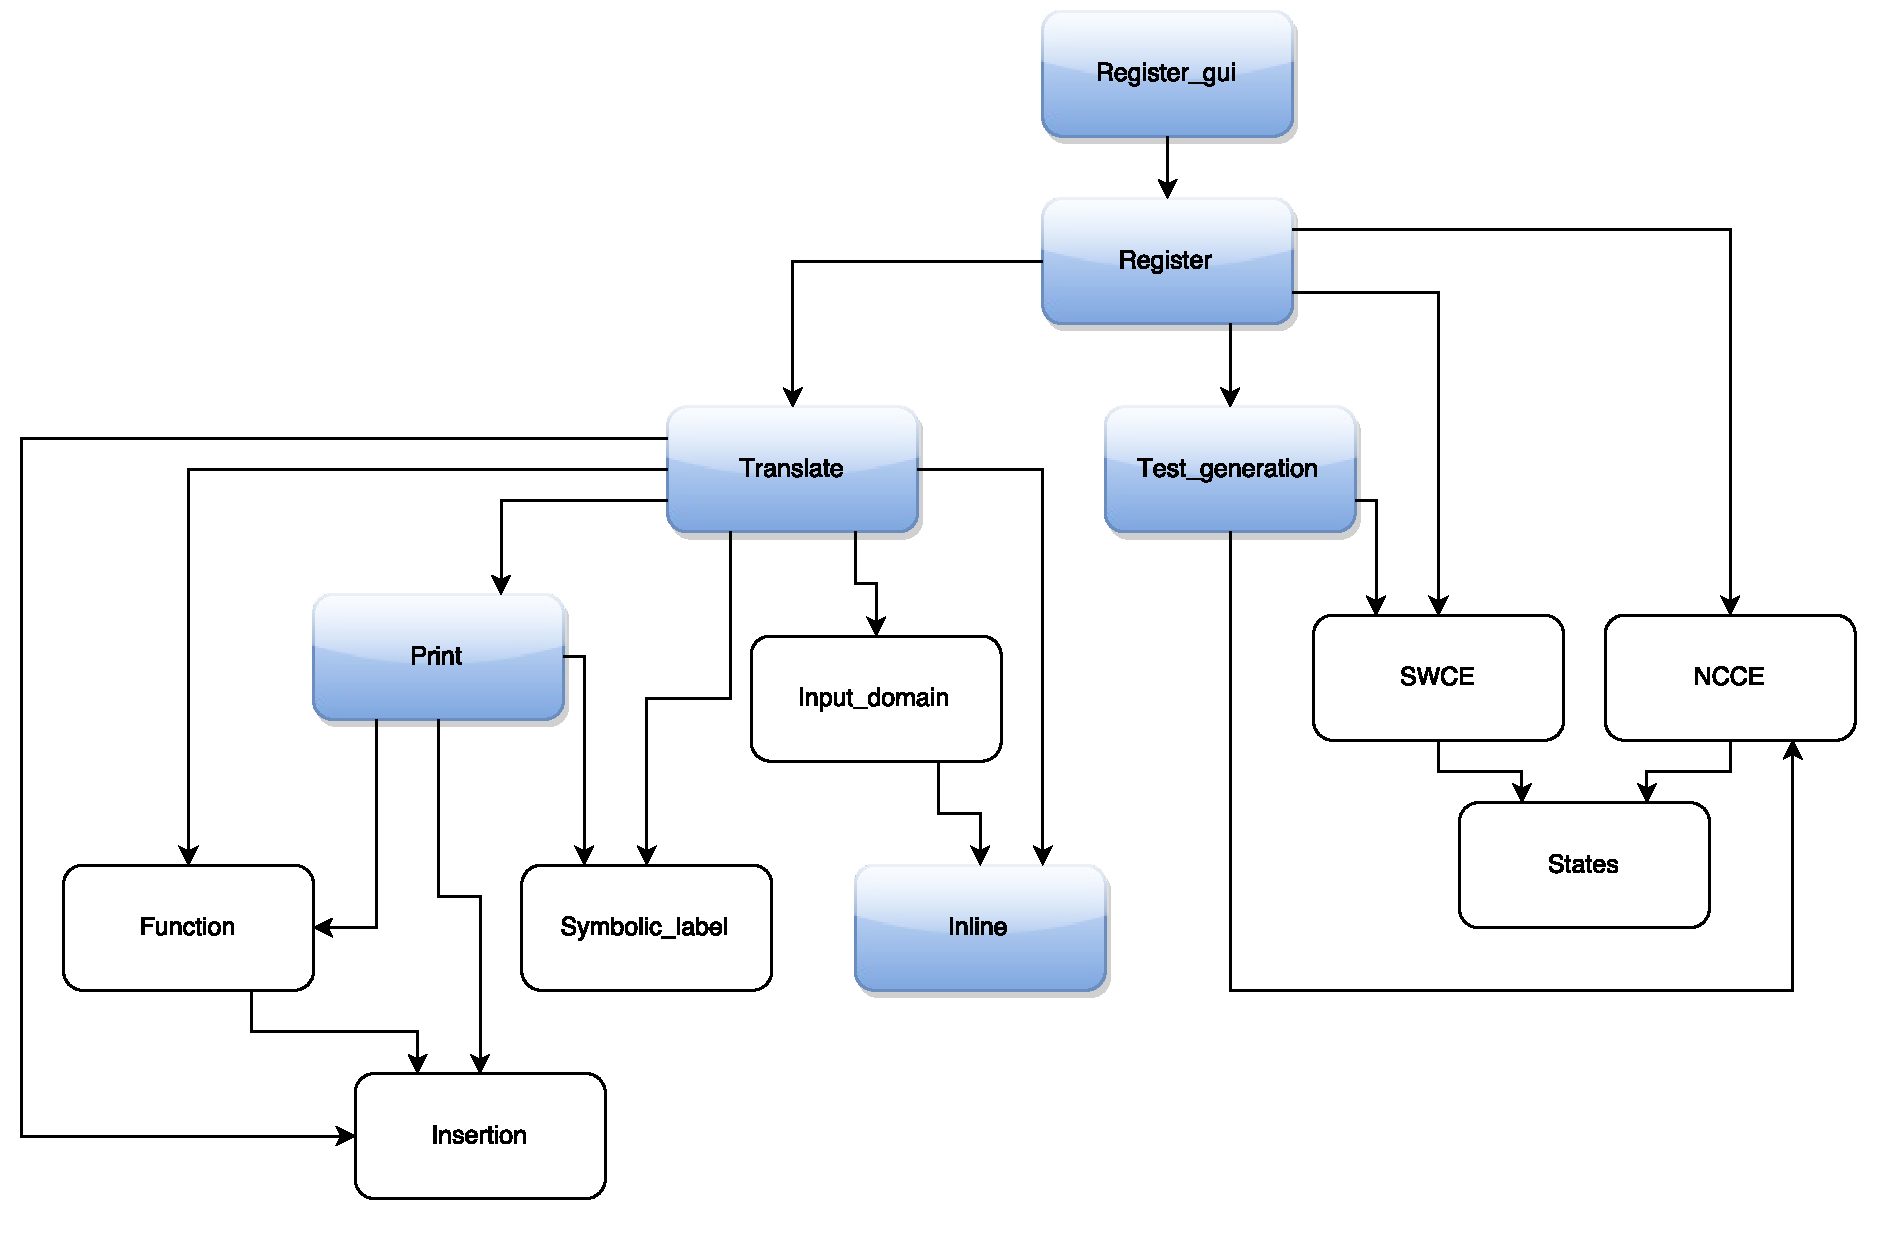
\includegraphics[scale=.5]{figures/stady_architecture.pdf}
    \vspace{-11cm}
    \caption{Architecture de \textsc{StaDy}
      \label{fig:stady-architecture}}
  \end{figure}
\end{center}
%\end{landscape}


\section{Expérimentations}


\begin{figure}[tb]\scriptsize
  %\vspace{-2mm}
  \begin{center}
    \begin{tabular}{lrr}
      \hline
      example & time (s.) & \# paths \\ \hline
      array-unsafe & 1.299 & 9 \\ \hline
      count-up-down-unsafe & 1.285 & 3 \\ \hline
      eureka-01-unsafe & 1.355 & 48 \\ \hline
      for-bounded-loop1-unsafe & 1.320 & 11 \\ \hline
      insertion-sort-unsafe & 16.530 & 730 \\ \hline
      invert-string-unsafe & 1.359 & 48 \\ \hline
      linear-search-unsafe & 3.624 & 2766 \\ \hline
      matrix-unsafe & 1.367 & 22 \\ \hline
      nec20-unsafe & 1.463 & 1035 \\ \hline
      string-unsafe & 1.362 & 48 \\ \hline
      sum01-bug02-base-unsafe & 1.335 & 26 \\ \hline
      sum01-bug02-unsafe & 1.327 & 36 \\ \hline
      sum01-unsafe & 1.312 & 56 \\ \hline
      sum03-unsafe & 1.291 & 46 \\ \hline
      sum04-unsafe & 1.310 & 22 \\ \hline
      sum-array-unsafe & 1.358 & 14 \\ \hline
      %% trex01-unsafe & 1.561 \\ \hline
      trex03-unsafe & 1.358 & 21 \\ \hline
      sendmail-unsafe & 1.396 & 77 \\ \hline
      vogal-unsafe & 1.349 & 341 \\ \hline
    \end{tabular}
  \end{center}
  \vspace{-3mm}
  \caption{Experiments with \textsc{StaDy}: Bug detection}    
  \label{fig:scam-experiments1}
  \vspace{-3mm}
\end{figure}

\begin{figure}[tb]\scriptsize
  %\vspace{-2mm}
  \begin{center}
    \begin{tabular}{lrrrr}
      \hline
      example & mutants & $\lnot$ equiv. & killed & success rate \\ \hline
      merge-sort & 96  & 92 & 88 & 95.65\% \\ \hline
      merge-arrays & 68 & 63 & 59 & 93.65\% \\ \hline
      quick-sort & 130 & 130 & 130 & 100\% \\ \hline
      binary-search & 40 & 40 & 39 & 97.5\% \\ \hline
      bubble-sort & 52 & 49 & 42 & 85.71\% \\ \hline
      insertion-sort & 39 & 37 & 36 & 97.3\% \\ \hline
      array-safe & 18 & 16 & 15 & 93.75\% \\ \hline
      bubble-sort-safe & 64 & 58 & 55 & 94.83\% \\ \hline
      count-up-down-safe & 14 & 13 & 13 & 100\% \\ \hline
      eureka-01-safe & 60 & 60 & 60 & 100\% \\ \hline
      eureka-05-safe & 36 & 36 & 36 & 100\% \\ \hline
      insertion-sort-safe & 43 & 41 & 40 & 97.56\% \\ \hline
      invert-string-safe & 47 & 47 & 47 & 100\% \\ \hline
      linear-search-safe & 19 & 17 & 16 & 94.12\% \\ \hline
      matrix-safe & 30 & 27 & 25 & 92.59\% \\ \hline
      nc40-safe & 20 & 20 & 20 & 100\% \\ \hline
      nec40-safe & 20 & 20 & 20 & 100\% \\ \hline
      string-safe & 65 & 65 & 65 & 100\% \\ \hline
      sum01-safe & 14 & 14 & 13 & 92.86\% \\ \hline
      sum02-safe & 14 & 14 & 11 & 78.57\% \\ \hline
      sum03-safe & 10 & 10 & 10 & 100\% \\ \hline
      sum04-safe & 14 & 14 & 10 & 71.43\% \\ \hline
      sum-array-safe & 17 & 17 & 15 & 88.24\% \\ \hline
      trex03-safe & 56 & 56 & 56 & 100\% \\ \hline
      sendmail-safe & 31 & 31 & 31 & 100\% \\ \hline
      vogal-safe & 71 & 68 & 67 & 98.53\% \\ \hline
      \textbf{Total} & 1088 & 1054 & 1019 & \textbf{96.68\%} \\ \hline
    \end{tabular}
  \end{center}
  \vspace{-3mm}
  \caption{Experiments with \textsc{StaDy}: Mutation testing}
  \label{fig:scam-experiments2}
  \vspace{-3mm}
\end{figure}

The current implementation of  
\textsc{StaDy} supports a significant subset of \eacsl including
assertions, pre- and postconditions, loop invaliants and variants,
quantifications, logic functions, integral and pointer types, and
basic pointer operations. Pointer validity is currenty supported
only for input arrays and pointers.
\textsc{StaDy} currently  does not support 
\lstinline{assigns} clauses, \lstinline{\at} terms, 
real numbers, as well as advanced memory-related constructs
(e.g. \lstinline{\offset}), complex pointer
arithmetics such as \lstinline'p1-p2' or \lstinline'*(p-i)' and dynamic memory allocation  
due to the limitations of the underlying test generator. 
%Annotations involving reals
%($\mathbb{R}$) are not supported either.

To evaluate the efficiency of \textsc{StaDy} 
%to find counter-examples 
in a combined verification approach
(cf Sec. \ref{sec:motivations}),
we applied it on safe and unsafe programs from the TACAS 2014
Software Verification Competition%
\footnote{\url{https://svn.sosy-lab.org/software/sv-benchmarks/trunk/c/loops}}
%(selected from the subdirectory {\em loops})
%to evaluate its efficiency. 
First, we 
%tracked down bugs in faulty programs.
%We 
executed \textsc{StaDy} on 20 faulty programs that  handle arrays
with loops. The properties to invalidate originally 
expressed as C assertions, were manually rewritten in \textsc{E-ACSL}.
Adequate \textsc{E-ACSL} preconditions were also added. The programs
containing infinite loops and reachability properties to invalidate are not
handled by  \textsc{StaDy} due to the necessity to execute the program in
\textsc{Path\-Crawler}.
\textsc{Sta\-Dy}
 detected failures of all faulty properties in each considered program. 
Fig.~\ref{fig:scam-experiments1} illustrates the time taken to
invalidate the properties including all the steps of \textsc{Sta\-Dy}:
instrumentation from the \textsc{E-ACSL} specifications and test generation in
\textsc{PathCrawler}, and the number of explored paths.

Secondly, we used  mutation testing to evaluate the ability of \textsc{StaDy} to
find bugs in unsafe programs. % automatically generated from safe programs.
We selected 20 safe programs of the same benchmark, and 6
additional safe programs from our own benchmarks. All of them were annotated in
\textsc{E-ACSL}. They contain preconditions, postconditions, assertions,
memory-related properties, loop variants and invariants. We used mutation testing
on these safe programs to generate modified programs (\emph{mutants}) and see if
\textsc{StaDy} is able to \emph{kill} 
(i.e. to find errors in) these mutants. The
mutations performed on the source code mimic usual programming errors. They
include modifications of numerical and/or pointer arithmetic operators,
comparison operators, condition negation and logical operators ({\em and} and
{\em or}). Fig.~\ref{fig:scam-experiments2} gives the 
numbers of all and erroneous mutants, as well as 
the number and proportion of erroneous mutants killed by \textsc{StaDy}. 
\textsc{StaDy} showed 
an average success rate of 96.68\%, going up to 100\% on many examples.
The missing percents are mostly due to 
%the incompleteness of the specifications
%in some programs, explained by 
a currently incomplete support of \textsc{E-ACSL} features
by the underlying test generation tool.


%%%%%%%%%%%%%%%%%%%%%%%%%%%%%%%%%%%%%%%%%%%%%%%%%%%%%%%%%%%%

\begin{figure*}[bt]
  \scriptsize
\mbox{}\hspace{-20mm}
  \begin{center}
  \begin{tabular}{r|c|c|c|c|c|c|c|c|c|c|c|c|c|c|c}
    &&\multicolumn{3}{c|}{Proof}&\multicolumn{4}{c|}{\NCD}
    &\multicolumn{4}{c|}{\CWD}&\multicolumn{2}{c|}{$\NCD+\CWD$}&\\
    \hline
    \input{full_exp_latex_IEEE.csv}
  \end{tabular}
\end{center}
  \caption{Detailed experiments of proof failure diagnosis for mutants with \stady}
  \vspace{-.5cm}
  \label{tab:exp}
\end{figure*}


\textbf{Implementation.}
The proposed method for diagnosis of proof failures 
% detecting  non-compliances and contract weaknesses
%described in Sec.~\ref{sec:global-method} 
has been implemented as a \framac plugin, named \stady.
It relies on other plugins: \Wp~\citeframac for deductive
verification and \pathcrawler~\citepathcrawler for structural test generation.
\stady currently supports a significant subset of the \eacsl specification
language, including 
\lstinline'requires', \lstinline'ensures', 
\lstinline'behavior', \lstinline'assumes', 
\lstinline'loop invariant', \lstinline'loop variant' and
\lstinline'assert' clauses.
Quantified predicates
\lstinline[style=c]'\exists' and \lstinline[style=c]'\forall' and builtin terms
as \lstinline'\sum' or \lstinline'\numof' are translated as loops. 
Logic functions and named predicates are treated by inlining.
The \lstinline'\old' constructs are treated by saving the initial
values of formal parameters and global variables at the beginning of the
function. 
Validity checks of pointers are
partially supported due to the current limitation of the underlying test
generator: we can only check the validity of input pointers and global arrays.
The \lstinline'assigns' clauses are only taken into consideration during the
\CWD phase: we do not aim to find what is missing in the \lstinline'assigns'
clause (\NCD) because provers usually give sufficiently good feedback about it,
but we want to find what is unnecessary and could be removed from an
\lstinline'assigns' clause (\CWD).
Inductive predicates, recursive functions and floating-point numbers are
currently not supported and are part of our future work.

\textbf{The research questions} we address in our experiments are the following.

\vspace{-2mm}
\begin{itemize}
\item[\textbf{RQ1}]
Is \stady able to precisely diagnose most proof failures in C programs?
\item[\textbf{RQ2}]
What are the benefits of the \CWD extension (in particular, with respect to
\NCD)?
\item[\textbf{RQ3}]
Is \stady able to generate  \NCCE{}s or \CWCE{}s even with a partial testing coverage?
\item[\textbf{RQ4}]
Is \stady's execution time comparable to the time of an automatic proof?
\end{itemize}
\vspace{-2mm}



\textbf{Experimental protocol.} 
The evaluation used 20 annotated programs from \cite{ACSLbyExample},
whose size varies from 35 to 100 lines of annotated C code.
%binary\_search, binary\_search2, lower\_bound, upper\_bound, max\_element,
%max\_element2, max\_seq, min\_element, copy, fill, iota, replace\_copy,
%reverse\_copy, adjacent\_find, equal, equal2, equal3, find, find2 and mismatch.
These programs manipulate arrays, they are fully specified in \acsl and their
specification expresses non-trivial properties of C arrays. 
To evaluate the method
presented in Sec.~\ref{sec:global-method} and its implementation, we apply \stady on systematically
generated altered  versions (or \emph{mutants}) of correct C programs.
%We apply the method presented in Sec.~\ref{sec:method} and measure the
%efficiency of the classification performed by \stady.
%Each utants are generated for each considered program 
Each mutant program is obtained by performing a single modification (or \emph{mutation}) on the
initial program.
The mutations include: a binary operator modification in the code or in the
specification, a condition negation in the code, a relation modification in the
specification, a predicate negation in the specification, a partial loop invariant or
postcondition deletion in the specification.
In this study, we do not mutate the precondition of the function under verification, 
and restrict possible mutations on binary operators to avoid creating absurd
expressions, in particular for pointer arithmetics.


The first step tries to prove each mutant using \Wp. 
%(with a timeout high enough \commentNK{preciser}).
The proved mutants respect the specification and are classified as correct. 
% are equivalent to the original program. % NK: Not sure!
Second, we apply the \NCD method on the remaining mutants.
It classifies proof failures for some mutants as non-compliances, indicates the failing annotation and an \NCCE.
The third step applies the \CWD method on remaining mutants,
classifies some of them as subcontract weaknesses, indicates the weak subcontract and a \CWCE.
If no counter-example has been found by the \CWD, the mutant remains 
unclassified. % (the \textsf{?} column).
%\commentNK{preciser timeouts here}
The results are displayed in Fig.~\ref{tab:exp}.
The columns 
%of  Fig.~\ref{tab:exp}  
present the number of generated mutants, and the results of each of the three
steps: the number (\#) and ratio (\%) of classified mutants,
maximal and average execution time (put on two lines) of the step
over classified mutants ($t^\text{\ok}$ or $t^\text{\ko}$) and over non-classified
mutants ($t^\text{?}$) at this step.
The ratios are computed with respect to unclassified mutants after the previous step.
The $\NCD+\CWD$ columns sum up selected results after both $\NCD$ and $\CWD$ steps:
the average and maximal time ($t$) are shown globally over all mutants.
The time is computed until the proof is finished or until the first counter-example is generated.
The final number of remaining unclassified mutants (\#?) is given in the last column.


\textbf{Experimental results.}
%\textbf{RQ1.}
%Regarding RQ1,
For the 20 considered programs, 928 mutants have been generated. 80 of them 
%are equivalent and 
have been proved by \Wp.
Among the 848 unproven mutants, \NCD has detected a non-compliance
induced by the mutation in 776 mutants (91.5\%),
leaving 72 unclassified.
Among them, \CWD has been able to exhibit a counter-example (either a \NCCE or a
\CWCE)
%, the confirmation step is not automatized yet) %NK: to be done for the final version
%for the contract impacted by
%the mutation in
for 48 of them (66.7\%), finally leaving 24 programs unclassified.
They can be either equivalent mutants that were not proved
by \Wp due to a prover incapacity, or mutants coming from a mutation 
in an unsupported annotation being undetectable by the
current version, or incorrect mutants for which testing was incomplete due to a timeout.
Regarding \textbf{RQ1}, \stady has found a precise reason
of the proof failures  and produced a counter-example 
in 824 of the 848 unproven mutants, 
i.e. classifying 97.2\%.
Exploring the benefits of detecting a prover incapacity may often require to manually reduce
the input domain, to try additional lemmas or interactive proof, so it   
was not sufficiently investigated in this study 
(and would probably require another, non mutational approach).

%\textbf{RQ2.}
Regarding \textbf{RQ2}, 
\NCD alone diagnosed 776 of 848 unproven mutants (91.5\%).
\CWD diagnosed 48 of the 72 remaining  mutants (66.7\%)
bringing a significant complementary contribution 
to a better understanding of reasons of many proof failures.
%The combined efforts of \NCD and \CWD classified 824 of 848 non-equivalent mutants
%(97.2\%), so \CWD permitted to add roughly 6\% to the fault detection efficiency
%of \NCD.

%\textbf{RQ3.}
In our experiments,
each prover can try to prove each verification condition 
%proof obligation 
during at most 40 seconds.
We also set a timeout for any test generation session
to 5 seconds, i.e. one session for the \NCD step, and 
several sessions for \CWD steps.
We also limit the depth of explored program paths with the 
{\em k-path} criterion (cf. Sec. \ref{sec:framac})
%With this option, the test generator only considers paths with at most
%$k$ consecutive iterations of each loop. 
setting $k = 4$.
Both the session timeout and the {\em k-path} heavily limit the testing coverage
but \stady still detects 97.2\% of faults in the generated programs.
That addresses \textbf{RQ3} and demonstrates that the proposed method can efficiently 
classify proof failures and generate counter-examples
even with a partial testing coverage and can therefore 
be used for programs where the 
total number of paths cannot be limited
(e.g. by the \lstinline{typically} clause).

%\textbf{Time of analysis.}
Concerning \textbf{RQ4},
on the considered programs \Wp needs on average 2.6 sec. per mutant (at most 4.4 sec.) to
prove a program, and spends 13.0 sec. on average (at most 61.3 sec.) when the
proof fails.
The total execution time of \stady is comparable: it needs on average 2.7 sec.  per unproven mutant 
(at most 19.9 sec.).
%More precisely, the \NCD step needed 2.4 sec. on average (at most 9.4 sec.) to
%detect a non-compliance, and on average 2.5 sec. (at most 8.3 sec.) when it is
%non conclusive.
%The \CWD step needed 2.4 sec. on average (at most 6.4 sec.) to
%detect a contract weakness, and on average 6.3 sec. (at most 11.6 sec.) when it
%is non conclusive.

\textbf{Summary.}
The experiments show that the proposed method can automatically classify a significant number
of proof failures within an analysis time comparable to the time of an automatic proof
and for programs for which only a partial testing coverage is possible.
The \CWD technique offers an efficient complement to \NCD for a more 
complete and more precise diagnosis of proof failures.

\textbf{Threats to validity.}
As it is often the case in software verification studies, one major threat is
related to the 
representativeness of results, i.e. their \textit{external validity}.
In our case, due to the nature of the problem,
we are restricted to realistic annotated programs
that cannot be generated automatically 
or extracted from existing databases of unspecified code.
Therefore, to reduce this threat, we used programs from an \textit{independent}
benchmark \cite{ACSLbyExample} created in order to illustrate
on different examples the usage of the \acsl specification 
language for deductive verification with \framac.


%Though, the primary contribution of this article is to propose 
%a novel classification of proof failures and techniques
%for their classification.

\textit{Scalability} of the results is another threat
since we do not demonstrate their validity for functions of larger programs. 
%While this is an important issue we plan to address in the near future, 
%However,  
Because of the modular reasoning of deductive verification,
it can be argued that the proposed technique should only be applied on a unit level,
separately for each function, since the verification engineer proves a program  in this way.
Indeed, in the current practice of deductive verification, it does not make sense to analyze
proof failures for the whole module or application at the same time.

The main scalability concern is thus related to the usage of structural test generation 
that can often time out without achieving a full coverage.
To address this issue, we have specifically investigated the impact of a partial test coverage
on the effectiveness of the method (cf. \textbf{RQ3} above) and proposed
a convenient way to reduce the input domain (using \lstinline{typically} clause, 
an extension of \acsl).

Other threats can be due to the used measurements, i.e. \textit{construct validity}.
To reduce this threat, we used a careful measurement of 
results (including analysis time for each step and 
each mutant, their mean and maximal values, 
separately computed for classified and unclassified proof failures).
One concern is producing realistic situations in which 
the verification engineer can need help in the analysis of proof failures.
While the first users of \stady have appreciated its feedback, % \cite{ggp15},
we have not yet had the opportunity to organize a fair evaluation with a 
representative group of users. 
Thus we have performed an extended set of experiments using simulation of 
errors by mutations as an alternative in the meanwhile. 
We have chosen a large subset of mutation operators (mutation in the code,
mutation in an annotation, deletion of an annotation) that model 
frequent problematic situations 
(incorrect code or annotations, incomplete specification)
leading to proof failures.
This approach looks suitable for non-compliance and subcontract weaknesses, and
certainly less suitable for the more subtle prover incapacity cases.
The results should be later confirmed by a representative user study.


\section*{Conclusion du chapitre}


TODO


\chapter{Bibliothèque de monitoring de la mémoire d'E-ACSL2C}
\label{sec:eacsl}

\chapterintro


Dans ce chapitre nous présentons notre implémentation du modèle mémoire des
programmes C qui permet d'exécuter les annotations \eacsl présentées dans
le chapitre~\ref{sec:runtime}.
Notre bibliothèque permet au greffon \eacsltoc de vérifier à l'exécution les
annotations \eacsl portant sur le modèle mémoire.

\eacsltoc traduit automatiquement un programme C annoté en un autre
programme C dont l'exécution échouera si une annotation n'est pas valide.
Si aucune annotation n'est violée, le comportement
du nouveau programme est exactement le même que celui du programme d'origine.
Ce greffon utilise notre bibliothèque afin de vérifier à l'exécution les
annotations \eacsl portant sur la mémoire.
Le greffon \eacsltoc lui-même n'étant pas le fruit de nos travaux
\cite{Delahaye/SAC13}, il ne sera pas présenté dans ce chapitre.

Nous présentons la bibliothèque en partie~\ref{sec:eacsl-impl}.
Au cours de nos travaux, nous avons mesuré la capacité de détection d'erreur de
notre implémentation et nous avons comparé les performances à l'exécution de
plusieurs choix d'implémentation.
Nous présentons les résultats de nos expérimentations en
partie~\ref{sec:eacsl-exp}.


\section{Architecture de la bibliothèque de monitoring de la mémoire}
\label{sec:eacsl-impl}


La figure~\ref{fig:mmodel-architecture} présente l'architecture générale de la
bibliothèque au moyen du graphe de dépendance des fonctions C les plus
importantes.
Une flèche $A \rightarrow B$ signifie que la fonction $A$ appelle la fonction
$B$.

\begin{figure}[h!]
  \centering
  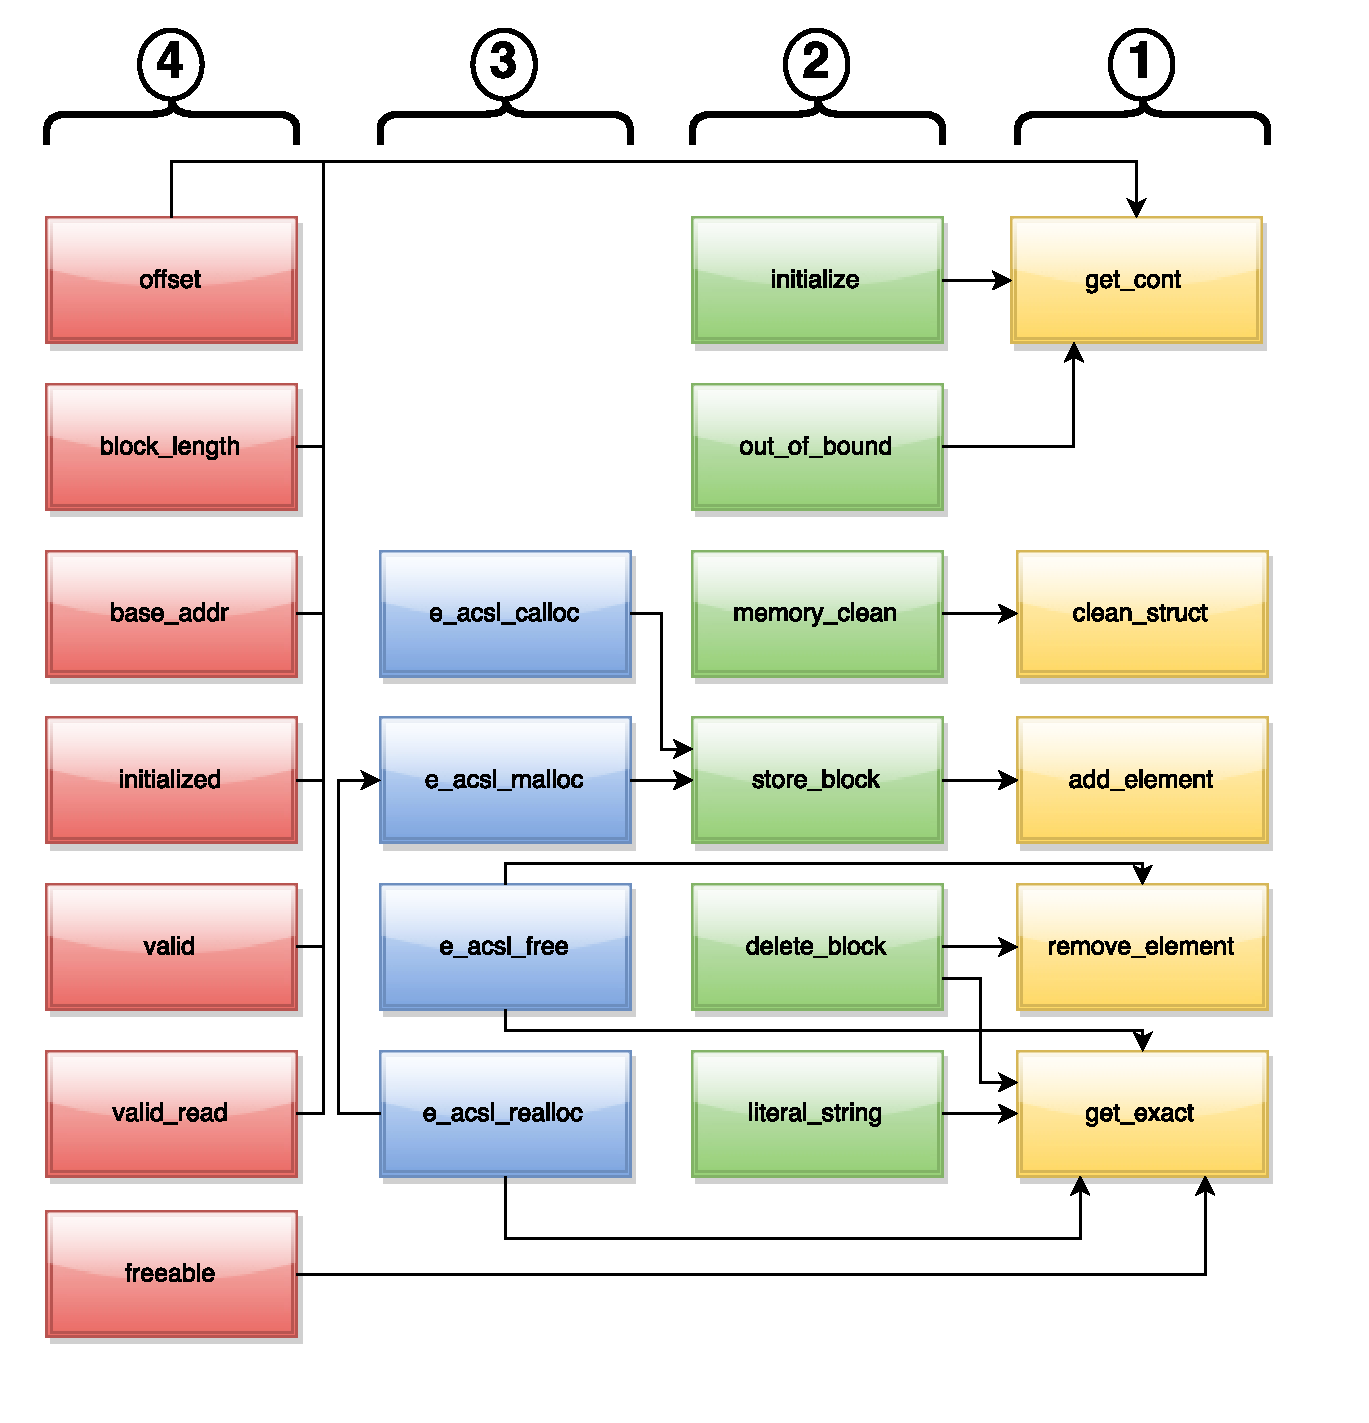
\includegraphics[scale=.55]{figures/mmodel_architecture.pdf}
  \vspace{-.8cm}
  \caption{Architecture de la bibliothèque de monitoring de la mémoire
    \label{fig:mmodel-architecture}}
\end{figure}

L'architecture comporte quatre niveaux, numérotés de \circled{1} à \circled{4}.
Les fonctions du niveau \circled{1} correspondent à l'implémentation de la
structure de données {\em store} (présentée au chapitre~\ref{sec:runtime})
gardant les informations à propos des blocs alloués.
Plusieurs implémentations sont fournies pour ces fonctions, correspondant à
différentes structures de données génériques : listes chaînées, arbres binaires
de recherche, Splay trees et Patricia tries.
Les fonctions du niveau \circled{2} servent à modifier le contenu du {\em store}
(ajout ou suppression d'élément, initialisation des éléments, etc.).
Les fonctions du niveau \circled{3} doivent être appelées en lieu et place des
fonctions de la bibliothèque standard associées (\lstinline'malloc', etc.).
Les fonctions du niveau \circled{4} permettent de calculer la valeur des
annotations \eacsl, elles retournent la valeur du terme ou du prédicat \eacsl
correspondant.
Ces fonctions ne modifient pas le contenu du {\em store}.

Les fonctions des niveaux \circled{2}, \circled{3} et \circled{4} sont
implémentées de manière indépendante à l'implémentation du {\em store} (niveau
\circled{1}).
Cette architecture facilite la conception des algorithmes, ainsi que la
comparaison d'efficacité des différentes implémentations du {\em store},
effectuée en partie~\ref{sec:eacsl-exp}.


\section{Expérimentations}
\label{sec:eacsl-exp}


Nous présentons maintenant le résultats de nos expérimentations visant à évaluer
la capacité de détection d'erreurs de la bibliothèque et la performance à
l'exécution des différents choix d'implémentation.


\subsection{Capacité de détection d'erreurs}


\begin{figure}
  \centering
  \begin{tabular}{c|c|c|c|c|c}
    & alarmes & mutants & équivalents & tués & \% erronés tués \\
    \hline
    fibonacci & 19  & 27 & 2 & 25 & 100\% \\
    \hline
    bubbleSort & 15  & 44 & 2 & 42 & 100\% \\
    \hline
    insertionSort & 10  & 39 & 3 & 36 & 100\% \\
    \hline
    binarySearch & 7 & 38 & 1 & 37 & 100\% \\
    \hline
    merge & 5 & 92 & 5 & 87 & 100\% \\
  \end{tabular}
  \caption{Capacité de détection d'erreurs
    \label{tab:mutation-exp}}
\end{figure}


Nous avons utilisé la technique de mutation pour évaluer la capacité de
détection d'erreurs en utilisant la vérification d'assertion à l'exécution avec
\framac.
Nous avons considéré 5 programmes écrits par nos soins.
Nous avons généré leurs {\em mutants} (en appliquant une {\em mutation} sur leur
code source) et leur avons appliqué la vérification à l'exécution.
Les mutations du programme incluent : modifications d'opérateur arithmétique
numérique, modifications d'opérateur arithmétique sur les pointeurs,
modifications d'opérateur de comparaison et modifications d'opérateur logique
($et$ et $ou$).
L'outil de génération de test \pathcrawler \cite{\citepathcrawler} a été
utilisé pour produire les cas de test.
Chaque mutant a été instrumenté par \eacsltoc et exécuté sur chaque cas de test
pour vérifier que la spécification était satisfaite à l'exécution.
Les programmes d'origine passent toutes les vérifications à l'exécution.
Lorsqu'une violation d'une annotation a été reportée pour au moins un cas de
test, le mutant est considéré comme étant {\em tué}.
La figure~\ref{tab:mutation-exp} présente les résultats.
La première colonne contient les exemples étudiés.
La deuxième colonne contient le nombre d'annotations dans chaque programme,
générées par interprétation abstraite (le greffon \Value a été utilisé).
Les colonnes suivantes contiennent le nombre de mutants générés, le nombre de
mutants équivalents, le nombre de mutants non-équivalents tués, et le
pourcentage des mutants non-équivalents tués lors de l'exécution.
Lors de ces expérimentations, tous les mutants non-équivalents erronés ont été
tués, ce qui témoigne de la précision et de la complétude de notre méthode.


\subsection{Performance des choix d'implémentation}


Pour évaluer la performance à l'exécution de notre implémentation de la
bibliothèque, nous avons effectué plus de 300 exécutions sur plus de 30
programmes, obtenus à partir d'une dizaine de programmes écrits et annotés par
nos soins.
Nous avons volontairement gardé des exemples plutôt courts (moins de 200 lignes
de code) car ils ont dû être annotés en \eacsl manuellement.

Nous avons mesuré le temps d'exécution du programme d'origine et du code
instrumenté par \eacsltoc avec différentes options, afin d'évaluer les
performances des différentes implémentations du {\em store} et des différentes
optimisations.
Des indicateurs comme le nombre de variables, d'allocations mémoires,
d'enregistrements et de requêtes ont également été enregistrés.


\textbf{Calcul du plus grand préfixe commun :} \\
Nous avons comparé deux implémentations de ce calcul, qui est utilisé par
l'implémentation du {\em store} utilisant des Patricia tries.
La première implémentation utilise un parcours linéaire de l'adresse (bit-à-bit,
de gauche à droite).
La seconde implémentation est une recherche dichotomique du meilleur préfixe
dans un tableau dont le contenu et les indices sont pré-calculés.
Elle implémente l'algorithme~\ref{algo:prefix} présenté en
partie~\ref{sec:mpgpc}.
Cette seconde implémentation s'est révélée en moyenne 2.7 fois plus rapide que
la première sur nos exemples.


\begin{figure}[h!]
  \begin{tikzpicture}
    \begin{axis}[axis y line=left,width=\textwidth,height=\textwidth,ymode=log,
        legend columns=2,xlabel={$N$},ylabel={temps (s.)}]
      \pgfplotstableread{data/table_eacsl_experiments_merge_sort.dat}
      \loadedtable;
      \addplot [color=red,ultra thick] table[x=N,y=list] {\loadedtable}
      node[above,pos=1] {list};

      \addplot [color=red,dashed,ultra thick]
      table[x=N,y=list-DFA] {\loadedtable}
      node[below,left,pos=1,yshift=-.5cm] {list-AS};

      \addplot [color=blue,ultra thick] table[x=N,y=bst] {\loadedtable}
      node[above,right,pos=1] {bst};

      \addplot [color=blue,dashed,ultra thick]
      table[x=N,y=bst-DFA] {\loadedtable}
      node[above,right,pos=1] {bst-AS};

      \addplot [color=greenv,ultra thick] table[x=N,y=Pt] {\loadedtable}
      node[above,left,pos=1,xshift=-1.4cm] {Pt};

      \addplot [color=greenv,dashed,ultra thick]
      table[x=N,y=Pt-DFA] {\loadedtable}
      node[above,left,pos=1] {Pt-dicho};

      \addplot [color=orange,ultra thick] table[x=N,y=Pt-opti] {\loadedtable}
      node[below,right,pos=1,yshift=-.5cm,xshift=-1.2cm] {Pt-AS};

      \addplot [color=orange,dashed,ultra thick]
      table[x=N,y=Pt-opti-DFA] {\loadedtable}
      node[above,left,pos=1] {Pt-dicho-AS};

      \addplot [color=violet,ultra thick] table[x=N,y=St] {\loadedtable}
      node[below,right,pos=1] {St};

      \addplot [color=violet,dashed,ultra thick]
      table[x=N,y=St-DFA] {\loadedtable}
      node[below,right,pos=1,yshift=-.7cm] {St-AS};

      %% \foreach \i in {
      %%   list,list-DFA,bst,bst-DFA,Pt,Pt-opti,Pt-DFA,Pt-opti-DFA,St,St-DFA} {
      %%   \addplot table [x=N, y=\i] {\loadedtable};
      %% }

      \legend{list,list-AS,bst,bst-AS,Pt,Pt-dicho,Pt-AS,Pt-dicho-AS,St,St-AS}
    \end{axis}
  \end{tikzpicture}
  \vspace{-.8cm}
  \caption{Comparaison du temps d'exécution des différentes implémentations du
    {\em store} sur un tri fusion
    \label{fig:mmodel-exp}}
\end{figure}


%% \begin{figure}[bt]
%%   \begin{tikzpicture}
%%     \begin{axis}[axis y line=left,width=\textwidth,height=\textwidth,ymode=log]
%%       \pgfplotstableread{data/table_eacsl_experiments_merge_sort.dat}
%%       \loadedtable;
%%       \foreach \i in {
%%         list,bst,Pt,Pt-opti,St} {
%%         \addplot table [x=N, y=\i] {\loadedtable};
%%       }
%%       \legend{list,bst,Pt$_1$,Pt$_2$,St}
%%     \end{axis}
%%   \end{tikzpicture}
%%   \caption{Comparaison des différentes implémentations du {\em store}
%%     \label{fig:mmodel-exp-2}}
%% \end{figure}


\textbf{Implémentation du {\em store} :}\\
Pour déterminer quelle implémentation du {\em store} est la plus appropriée,
nous avons comparé quatre implémentations utilisant : des Patricia tries, des
listes chaînées, des arbres binaires de recherche non équilibrés et des arbres
binaires de recherche équilibrés (Splay trees~\cite{Sleator/85}).

La figure~\ref{tab:mmodel-exp} présente les résultats des expérimentations
comparant les différentes implémentations du {\em store} et du calcul du plus
grand préfixe commun.
La première colonne du tableau contient les exemples étudiés.
$bS_{10000}$ est une recherche binaire dans un tableau de 10000 éléments.
$iS_{10000}$ est un tri par insertion d'un tableau de 10000 éléments.
$mM_{n^2}$ est une multiplication de matrices $n \times n$. mI$_{n^2}$ contient
des calculs matriciels (dont inversion et multiplication) sur des  matrices
$n \times n$.
$qS_n$ est un tri rapide sur un tableau de $n$ éléments.
$bbS_{10000}$ est un tri à bulle sur un tableau à 10000 éléments.
$m_{30000}$ est une fusion de deux listes chaînées de 10000 et 20000 éléments.
$Rbt_{10000}$ est une insertion/suppression de 10000 éléments dans un arbre rouge
et noir.
$mS_n$ est un tri fusion d'une liste chaînée de $n$ éléments.
La ligne supplémentaire ``+ RTE'' de chaque exemple correspond à une application
préalable du greffon \rte qui génère des assertions qui sont vraies si le
programme ne contient pas d'erreur à l'exécution.
Nous appelons ces assertions à vérifier des ``alarmes''.

La colonne $\danger$ contient le nombre d'alarmes du programme (générées par les
greffons \rte et \Value).
La colonne $\emptyset$ contient le temps d'exécution du programme original.
Tous les temps d'exécution sont mesurés en secondes.
Un temps d'exécution est noté $\infty$ quand il dépasse 24 heures.
Dans les colonnes suivantes, le suffixe ``-AS'' correspond aux expérimentations
avec application d'une analyse statique permettant de n'instrumenter que ce qui
est nécessaire (section 6 de \cite{\citeeacsltoc}).
Cette analyse n'étant pas le fruit de nos travaux, nous ne la présentons pas
ici.
La colonne $list$ contient le temps d'exécution du programme lorsque le
{\em store} est implémenté par une liste chaînée.
La colonne $bst$ contient le temps d'exécution du programme lorsque le
{\em store} est implémenté par un arbre binaire de recherche non équilibré.
La colonne $Pt$ contient le temps d'exécution du programme lorsque le
{\em store} est implémenté par un Patricia trie et lorsque la recherche du
masque du plus grand préfixe commun de deux adresses est implémentée de manière
linéaire.
La colonne $Pt-dicho$ contient le temps d'exécution du programme lorsque le
{\em store} est implémenté par un Patricia trie et lorsque la recherche du
masque du plus grand préfixe commun de deux adresses est implémentée en
utilisant l'algorithme~\ref{algo:prefix} présenté en partie~\ref{sec:mpgpc}.
La colonne $St$ contient le temps d'exécution du programme lorsque le
{\em store} est implémenté par un Splay tree.
Le temps d'analyse du programme sans instrumentation avec le débogueur
\valgrind~\cite{\citevalgrind} est indiqué dans la dernière colonne.

Nous remarquons que le temps d'exécution de \valgrind n'est pas comparable avec
celui de notre bibliothèque, cela s'explique simplement par le fait que celui-ci
ne prend pas en compte la spécification \eacsl, et se contente de vérifier des
propriétés comme l'absence d'erreur de segmentation ou l'absence de fuite de
mémoire.
En effet, notre démarche vise à supporter au maximum les annotations \eacsl,
ce qui nécessite un monitoring plus lourd.

La figure~\ref{fig:mmodel-exp} représente graphiquement le temps (en secondes)
passé par chaque implémentation du {\em store} sur un tri fusion de 1000, 5000,
10000, 50000 et 100000 éléments (les données chiffrées sont dans les cinq
dernières lignes de la figure~\ref{tab:mmodel-exp}).

Les résultats de nos expérimentations confirment nos hypothèses, à savoir :

\begin{itemize}
\item[\textbf{H1}]
  le Patricia trie est la structure de données la plus appropriée pour
  l'implémentation du {\em store};

\item[\textbf{H2}]
  notre optimisation de la recherche du masque du plus grand préfixe commun par
  recherche dichotomique et l'utilisation d'indices pré-calculés entraîne un
  vrai gain de performance;

\item[\textbf{H3}]
  l'utilisation d'une analyse statique visant à réduire l'instrumentation
  du programme permet de réduire le temps d'exécution de manière efficace.
\end{itemize}


Concernant \textbf{H1}, la figure~\ref{tab:mmodel-exp} montre que
l'implémentation du {\em store} par un Patricia trie est la plus efficace.
Elle est en moyenne 2500 fois plus rapide que l'implémentation à base de listes
chaînées, 200 fois plus rapide que celle utilisant les arbres binaires de
recherche, et 27 fois plus rapide que celle se basant sur les Splay trees.

La version utilisant les Splay trees offre des performances comparables (ou
légèrement meilleures, jusqu'à 3 fois) sur les exemples contenant de fréquents
accès mémoire consécutifs au même bloc dans le {\em store}, comme c'est le cas
du tri fusion (voir la figure~\ref{fig:mmodel-exp}).
En revanche, sur des exemples où les accès mémoire consécutifs ne se font pas
sur le même bloc (une multiplication de matrices dans notre exemple), les
performances sont beaucoup moins bonnes (jusqu'à 500 fois).
Ceci est dû à la nature des Splay trees : le dernier élément accédé est remonté
à la racine de l'arbre.

Concernant \textbf{H2}, la figure~\ref{tab:mmodel-exp} montre que la version
dichotomique de la recherche du masque du plus grand préfixe commun est toujours
plus efficace qu'une recherche linéaire.
Elle est en moyenne 3 fois plus rapide que cette dernière.

Concernant \textbf{H3}, nos résultats montrent que l'utilisation d'une analyse
statique visant à réduire l'instrumentation du programme entraîne un gain de
performance.
En effet, pour chacune des implémentations du {\em store}, l'analyse statique
permet de réduire le temps d'exécution.
L'exécution après analyse statique peut être jusqu'à 200 fois plus rapide sur
certains exemples.
Elle permet notamment de ne pas observer de {\em timeout} pour les listes
chaînées et les arbres binaires de recherche sur l'exemple du tri fusion de
50000 éléments.


\section*{Conclusion du chapitre}


Dans ce chapitre nous avons présenté l'architecture de l'implémentation de la
bibliothèque de monitoring de la mémoire, dont les algorithmes et les principes
théoriques ont été traités dans le chapitre~\ref{sec:runtime}.

Nous avons présenté les résultats de nos expérimentations visant à
mesurer la capacité de détection d'erreurs et les performances à l'exécution de
notre implémentation.
Nous avons notamment comparé les performances de quatre implémentations du
{\em store}.
Nous avons également comparé deux implémentations de la recherche du masque du
plus grand préfixe commun, dans le cas où le {\em store} est implémenté en
utilisant un Patricia trie.
Enfin, nous avons mesuré l'impact de l'utilisation d'une analyse statique visant
à réduire l'instrumentation du programme (section 6 de \cite{\citeeacsltoc}),
pour chacune des implémentations du {\em store}.
Nos expérimentations ont mis en avant l'efficacité d'une implémentation du
{\em store} à base de Patricia trie.
Elles ont également montré qu'une recherche du masque du plus grand préfixe
commun par dichotomie (l'algorithme est présenté en partie~\ref{sec:mpgpc}) est
plus efficace qu'une recherche linéaire et que l'analyse statique permet
effectivement de réduire le temps de la vérification à l'exécution.

Le travail réalisé a permis de concevoir une méthode et un outil de vérification
à l'exécution des annotations \eacsl portant sur le modèle mémoire.
Nos travaux ont permis de déterminer expérimentalement quelles implémentations
du {\em store} et des différents algorithmes sont les plus efficaces pour notre
outil de vérification.
L'implémentation du {\em store} à base de Patricia trie et les différents
algorithmes présentés dans ce chapitre et dans le chapitre~\ref{sec:runtime}
sont intégrés à l'outil \eacsltoc~\cite{\citeeacsltoc}.


\begin{landscape}
  \begin{figure}[h]
    \centering
    \begin{footnotesize}
      \begin{tabular}{l|c|c|c|c|c|c|c|HHc|c|HHc|c|c|c}
  & $\danger$ & $\emptyset$ & list & list-AS & bst & bst-AS & Pt & mask$^1$ & sb$^1$ & Pt-dicho & Pt-AS & mask$^2$ & sb$^2$ & Pt-dicho-AS & St & St-AS & valgrind \\
  \hline
  bS$_{10000}$ &22 &\multirow{2}{*}{.01} &1.10 &0.50 &1.14 &0.64 &1.55 &99 &16 &1.55 &0.57 &0 &1 &0.55 &1.39 &0.61 &\multirow{2}{*}{0.27}\\
  + RTE &41 &&1.10 &0.51 &1.14 &0.62 &1.59 &109 &16 &1.59 &0.53 &0 &1 &0.53 &1.39 &0.64 &\\
  \hline
  iS$_{10000}$ &5 &\multirow{2}{*}{.12} &2.29 &0.12 &1.83 &0.12 &2.89 &170k &20k &2.91 &0.12 &0 &0 &0.12 &2.46 &0.12 &\multirow{2}{*}{2.81}\\
  + RTE &24 &&3.52 &1.27 &2.89 &1.26 &3.99 &170k &20k &3.86 &1.25 &0 &0 &1.25 &3.46 &1.30 &\\
  \hline
  mM$_{100^2}$ &0 &\multirow{2}{*}{.01} &2.29 &0.73 &2.94 &1.15 &0.14 &17k &1k &0.14 &0.10 &5k &612 &0.09 &1.07 &0.98 &\multirow{2}{*}{0.34}\\
  + RTE &82 &&13.17 &10.66 &21.92 &17.39 &2.78 &18k &1k &3.00 &2.64 &5k &612 &2.82 &75.97 &73.62 &\\
  \hline
  mM$_{150^2}$ &0 &\multirow{2}{*}{.01} &13.23 &3.96 &15.65 &6.20 &0.54 &21k &2k &0.51 &0.36 &9k &912 &0.35 &5.86 &5.64 &\multirow{2}{*}{0.48}\\
  + RTE &82 &&72.36 &58.48 &110.70 &90.43 &10.77 &24k &2k &9.01 &8.57 &9k &912 &8.75 &403.50 &398.60 &\\
  \hline
  mI$_{100^2}$ &2 &\multirow{2}{*}{.01} &22.51 &0.10 &7.74 &0.13 &0.09 &68k &5k &0.08 &0.01 &7k &609 &0.01 &0.19 &0.10 &\multirow{2}{*}{0.35}\\
  + RTE &155 &&28.96 &4.22 &13.67 &5.48 &0.54 &73k &5k &0.55 &0.53 &7k &611 &0.47 &26.37 &26.16 &\\
  \hline
  mI$_{150^2}$ &2 &\multirow{2}{*}{.02} &130.04 &0.34 &40.35 &0.45 &0.28 &99k &8k &0.27 &0.02 &12k &909 &0.02 &0.68 &0.34 &\multirow{2}{*}{0.47}\\
  + RTE &155 &&153.30 &21.54 &73.55 &29.94 &2.00 &105k &8k &1.90 &1.42 &12k &911 &1.53 &146.15 &145.80 &\\
  \hline
  qS$_{1000}$ &15 &\multirow{2}{*}{.01} &12.70 &2.08 &1.76 &0.59 &0.33 &1M &92k &0.06 &0.13 &683k &39k &0.02 &0.02 &0.01 &\multirow{2}{*}{0.27}\\
  + RTE &32 &&12.38 &2.13 &1.64 &0.56 &0.38 &1M &92k &0.12 &0.14 &727k &39k &0.04 &0.03 &0.02 &\\
  \hline
  qS$_{2000}$ &15 &\multirow{2}{*}{.01} &85.99 &11.31 &8.39 &2.78 &0.71 &3M &198k &0.14 &0.28 &1M &84k &0.05 &0.03 &0.02 &\multirow{2}{*}{0.27}\\
  + RTE &32 &&81.65 &11.15 &7.72 &2.67 &1.13 &4M &198k &0.48 &0.36 &1M &84k &0.13 &0.05 &0.02 &\\
  \hline
  bbS$_{10000}$ &4 &\multirow{2}{*}{.22} &13.78 &1.02 &16.84 &1.67 &117.47 &499M &49M &22.36 &1.57 &30 &7 &1.54 &8.80 &1.67 &\multirow{2}{*}{3.36}\\
  + RTE &16 &&23.08 &4.64 &30.69 &7.16 &107.05 &599M &49M &32.58 &7.26 &29 &7 &6.90 &17.29 &7.21 &\\
  \hline
  m$_{30000}$ &2 &\multirow{2}{*}{.01} &412.10 &11.38 &176.35 &11.01 &1.11 &5M &420k &0.26 &0.30 &1M &60k &0.06 &0.08 &0.01 &\multirow{2}{*}{0.45}\\
  + RTE &49 &&451.58 &101.33 &219.12 &94.80 &1.15 &5M &420k &0.29 &0.47 &2M &130k &0.14 &0.10 &0.05 &\\
  \hline
  Rbt$_{10000}$ &0 &\multirow{2}{*}{.01} &47.39 &0.28 &48.44 &0.27 &0.32 &1M &159k &0.09 &0.03 &151k &10k &0.01 &0.59 &0.01 &\multirow{2}{*}{0.51}\\
  + RTE &270 &&120.02 &101.69 &165.77 &145.20 &0.47 &1M &159k &0.30 &0.39 &979k &119k &0.27 &18.82 &19.59 &\\
  \hline
  mS$_{1000}$ &7 &\multirow{2}{*}{.01} &6.45 &0.34 &6.32 &0.11 &0.32 &1M &95k &0.07 &0.06 &331k &18k &0.01 &0.02 &0.01 &\multirow{2}{*}{0.27}\\
  + RTE &45 &&6.82 &1.35 &7.98 &0.38 &0.34 &1M &95k &0.10 &0.13 &701k &38k &0.04 &0.02 &0.01 &\\
  \hline
  mS$_{5000}$ &7 &\multirow{2}{*}{.01} &362.87 &11.00 &218.01 &3.43 &2.28 &11M &562k &0.76 &0.43 &2M &106k &0.09 &0.14 &0.03 &\multirow{2}{*}{0.27}\\
  + RTE &45 &&371.40 &50.94 &290.88 &10.34 &2.46 &11M &562k &0.80 &0.83 &4M &218k &0.22 &0.16 &0.08 &\\
  \hline
  mS$_{10000}$ &7 &\multirow{2}{*}{.01} &3624.01 &47.94 &1673.00 &16.10 &6.46 &23M &1M &2.75 &1.00 &5M &223k &0.21 &0.31 &0.08 &\multirow{2}{*}{0.27}\\
  + RTE &45 &&3406.43 &257.18 &2086.32 &46.22 &6.30 &23M &1M &2.66 &1.83 &9M &457k &0.51 &0.35 &0.18 &\\
  \hline
  mS$_{50000}$ &7 &\multirow{2}{*}{.01} &$\infty$ &3847.72 &$\infty$ &1100.93 &135.54 &146M &6M &111.22 &6.90 &33M &1M &1.65 &2.08 &0.58 &\multirow{2}{*}{0.63}\\
  + RTE &45 &&$\infty$ &25554.08 &$\infty$ &2781.90 &118.86 &145M &6M &95.74 &11.64 &54M &2M &3.37 &2.18 &1.15 &\\
  \hline
  mS$_{100000}$ &7 &\multirow{2}{*}{.01} &$\infty$ &$\infty$ &$\infty$ &$\infty$ &631.41 &296M &14M &559.93 &13.55 &70M &2M &3.35 &4.03 &1.15 &\multirow{2}{*}{0.27}\\
  + RTE &45 &&$\infty$ &$\infty$ &$\infty$ &$\infty$ &573.47 &308M &14M &513.85 &25.02 &116M &5M &7.63 &4.68 &2.50 &\\
\end{tabular}

    \end{footnotesize}
    \caption{Comparaison des différentes implémentations du {\em store}
      \label{tab:mmodel-exp}}
  \end{figure}
\end{landscape}



\part{Conclusion}
\chapter{Bilan}
TODO
\chapter{Perspectives}
TODO


\backmatter

\bibliographystyle{phdthesisapa}
\bibliography{biblio}

\listoffigures
\listoftables
\listofdefinitions

\appendix
\part{Annexes}

\chapter{Premier chapitre des annexes}
\chapter{Second chapitre des annexes}

\end{document}

